
% Default to the notebook output style

    


% Inherit from the specified cell style.




    
\documentclass[11pt]{article}

    
    
    \usepackage[T1]{fontenc}
    % Nicer default font (+ math font) than Computer Modern for most use cases
    \usepackage{mathpazo}

    % Basic figure setup, for now with no caption control since it's done
    % automatically by Pandoc (which extracts ![](path) syntax from Markdown).
    \usepackage{graphicx}
    % We will generate all images so they have a width \maxwidth. This means
    % that they will get their normal width if they fit onto the page, but
    % are scaled down if they would overflow the margins.
    \makeatletter
    \def\maxwidth{\ifdim\Gin@nat@width>\linewidth\linewidth
    \else\Gin@nat@width\fi}
    \makeatother
    \let\Oldincludegraphics\includegraphics
    % Set max figure width to be 80% of text width, for now hardcoded.
    \renewcommand{\includegraphics}[1]{\Oldincludegraphics[width=.8\maxwidth]{#1}}
    % Ensure that by default, figures have no caption (until we provide a
    % proper Figure object with a Caption API and a way to capture that
    % in the conversion process - todo).
    \usepackage{caption}
    \DeclareCaptionLabelFormat{nolabel}{}
    \captionsetup{labelformat=nolabel}

    \usepackage{adjustbox} % Used to constrain images to a maximum size 
    \usepackage{xcolor} % Allow colors to be defined
    \usepackage{enumerate} % Needed for markdown enumerations to work
    \usepackage{geometry} % Used to adjust the document margins
    \usepackage{amsmath} % Equations
    \usepackage{amssymb} % Equations
    \usepackage{textcomp} % defines textquotesingle
    % Hack from http://tex.stackexchange.com/a/47451/13684:
    \AtBeginDocument{%
        \def\PYZsq{\textquotesingle}% Upright quotes in Pygmentized code
    }
    \usepackage{upquote} % Upright quotes for verbatim code
    \usepackage{eurosym} % defines \euro
    \usepackage[mathletters]{ucs} % Extended unicode (utf-8) support
    \usepackage[utf8x]{inputenc} % Allow utf-8 characters in the tex document
    \usepackage{fancyvrb} % verbatim replacement that allows latex
    \usepackage{grffile} % extends the file name processing of package graphics 
                         % to support a larger range 
    % The hyperref package gives us a pdf with properly built
    % internal navigation ('pdf bookmarks' for the table of contents,
    % internal cross-reference links, web links for URLs, etc.)
    \usepackage{hyperref}
    \usepackage{longtable} % longtable support required by pandoc >1.10
    \usepackage{booktabs}  % table support for pandoc > 1.12.2
    \usepackage[inline]{enumitem} % IRkernel/repr support (it uses the enumerate* environment)
    \usepackage[normalem]{ulem} % ulem is needed to support strikethroughs (\sout)
                                % normalem makes italics be italics, not underlines
    

    
    
    % Colors for the hyperref package
    \definecolor{urlcolor}{rgb}{0,.145,.698}
    \definecolor{linkcolor}{rgb}{.71,0.21,0.01}
    \definecolor{citecolor}{rgb}{.12,.54,.11}

    % ANSI colors
    \definecolor{ansi-black}{HTML}{3E424D}
    \definecolor{ansi-black-intense}{HTML}{282C36}
    \definecolor{ansi-red}{HTML}{E75C58}
    \definecolor{ansi-red-intense}{HTML}{B22B31}
    \definecolor{ansi-green}{HTML}{00A250}
    \definecolor{ansi-green-intense}{HTML}{007427}
    \definecolor{ansi-yellow}{HTML}{DDB62B}
    \definecolor{ansi-yellow-intense}{HTML}{B27D12}
    \definecolor{ansi-blue}{HTML}{208FFB}
    \definecolor{ansi-blue-intense}{HTML}{0065CA}
    \definecolor{ansi-magenta}{HTML}{D160C4}
    \definecolor{ansi-magenta-intense}{HTML}{A03196}
    \definecolor{ansi-cyan}{HTML}{60C6C8}
    \definecolor{ansi-cyan-intense}{HTML}{258F8F}
    \definecolor{ansi-white}{HTML}{C5C1B4}
    \definecolor{ansi-white-intense}{HTML}{A1A6B2}

    % commands and environments needed by pandoc snippets
    % extracted from the output of `pandoc -s`
    \providecommand{\tightlist}{%
      \setlength{\itemsep}{0pt}\setlength{\parskip}{0pt}}
    \DefineVerbatimEnvironment{Highlighting}{Verbatim}{commandchars=\\\{\}}
    % Add ',fontsize=\small' for more characters per line
    \newenvironment{Shaded}{}{}
    \newcommand{\KeywordTok}[1]{\textcolor[rgb]{0.00,0.44,0.13}{\textbf{{#1}}}}
    \newcommand{\DataTypeTok}[1]{\textcolor[rgb]{0.56,0.13,0.00}{{#1}}}
    \newcommand{\DecValTok}[1]{\textcolor[rgb]{0.25,0.63,0.44}{{#1}}}
    \newcommand{\BaseNTok}[1]{\textcolor[rgb]{0.25,0.63,0.44}{{#1}}}
    \newcommand{\FloatTok}[1]{\textcolor[rgb]{0.25,0.63,0.44}{{#1}}}
    \newcommand{\CharTok}[1]{\textcolor[rgb]{0.25,0.44,0.63}{{#1}}}
    \newcommand{\StringTok}[1]{\textcolor[rgb]{0.25,0.44,0.63}{{#1}}}
    \newcommand{\CommentTok}[1]{\textcolor[rgb]{0.38,0.63,0.69}{\textit{{#1}}}}
    \newcommand{\OtherTok}[1]{\textcolor[rgb]{0.00,0.44,0.13}{{#1}}}
    \newcommand{\AlertTok}[1]{\textcolor[rgb]{1.00,0.00,0.00}{\textbf{{#1}}}}
    \newcommand{\FunctionTok}[1]{\textcolor[rgb]{0.02,0.16,0.49}{{#1}}}
    \newcommand{\RegionMarkerTok}[1]{{#1}}
    \newcommand{\ErrorTok}[1]{\textcolor[rgb]{1.00,0.00,0.00}{\textbf{{#1}}}}
    \newcommand{\NormalTok}[1]{{#1}}
    
    % Additional commands for more recent versions of Pandoc
    \newcommand{\ConstantTok}[1]{\textcolor[rgb]{0.53,0.00,0.00}{{#1}}}
    \newcommand{\SpecialCharTok}[1]{\textcolor[rgb]{0.25,0.44,0.63}{{#1}}}
    \newcommand{\VerbatimStringTok}[1]{\textcolor[rgb]{0.25,0.44,0.63}{{#1}}}
    \newcommand{\SpecialStringTok}[1]{\textcolor[rgb]{0.73,0.40,0.53}{{#1}}}
    \newcommand{\ImportTok}[1]{{#1}}
    \newcommand{\DocumentationTok}[1]{\textcolor[rgb]{0.73,0.13,0.13}{\textit{{#1}}}}
    \newcommand{\AnnotationTok}[1]{\textcolor[rgb]{0.38,0.63,0.69}{\textbf{\textit{{#1}}}}}
    \newcommand{\CommentVarTok}[1]{\textcolor[rgb]{0.38,0.63,0.69}{\textbf{\textit{{#1}}}}}
    \newcommand{\VariableTok}[1]{\textcolor[rgb]{0.10,0.09,0.49}{{#1}}}
    \newcommand{\ControlFlowTok}[1]{\textcolor[rgb]{0.00,0.44,0.13}{\textbf{{#1}}}}
    \newcommand{\OperatorTok}[1]{\textcolor[rgb]{0.40,0.40,0.40}{{#1}}}
    \newcommand{\BuiltInTok}[1]{{#1}}
    \newcommand{\ExtensionTok}[1]{{#1}}
    \newcommand{\PreprocessorTok}[1]{\textcolor[rgb]{0.74,0.48,0.00}{{#1}}}
    \newcommand{\AttributeTok}[1]{\textcolor[rgb]{0.49,0.56,0.16}{{#1}}}
    \newcommand{\InformationTok}[1]{\textcolor[rgb]{0.38,0.63,0.69}{\textbf{\textit{{#1}}}}}
    \newcommand{\WarningTok}[1]{\textcolor[rgb]{0.38,0.63,0.69}{\textbf{\textit{{#1}}}}}
    
    
    % Define a nice break command that doesn't care if a line doesn't already
    % exist.
    \def\br{\hspace*{\fill} \\* }
    % Math Jax compatability definitions
    \def\gt{>}
    \def\lt{<}
    % Document parameters
    \title{TP\_Images\_2020}
    
    
    

    % Pygments definitions
    
\makeatletter
\def\PY@reset{\let\PY@it=\relax \let\PY@bf=\relax%
    \let\PY@ul=\relax \let\PY@tc=\relax%
    \let\PY@bc=\relax \let\PY@ff=\relax}
\def\PY@tok#1{\csname PY@tok@#1\endcsname}
\def\PY@toks#1+{\ifx\relax#1\empty\else%
    \PY@tok{#1}\expandafter\PY@toks\fi}
\def\PY@do#1{\PY@bc{\PY@tc{\PY@ul{%
    \PY@it{\PY@bf{\PY@ff{#1}}}}}}}
\def\PY#1#2{\PY@reset\PY@toks#1+\relax+\PY@do{#2}}

\expandafter\def\csname PY@tok@w\endcsname{\def\PY@tc##1{\textcolor[rgb]{0.73,0.73,0.73}{##1}}}
\expandafter\def\csname PY@tok@c\endcsname{\let\PY@it=\textit\def\PY@tc##1{\textcolor[rgb]{0.25,0.50,0.50}{##1}}}
\expandafter\def\csname PY@tok@cp\endcsname{\def\PY@tc##1{\textcolor[rgb]{0.74,0.48,0.00}{##1}}}
\expandafter\def\csname PY@tok@k\endcsname{\let\PY@bf=\textbf\def\PY@tc##1{\textcolor[rgb]{0.00,0.50,0.00}{##1}}}
\expandafter\def\csname PY@tok@kp\endcsname{\def\PY@tc##1{\textcolor[rgb]{0.00,0.50,0.00}{##1}}}
\expandafter\def\csname PY@tok@kt\endcsname{\def\PY@tc##1{\textcolor[rgb]{0.69,0.00,0.25}{##1}}}
\expandafter\def\csname PY@tok@o\endcsname{\def\PY@tc##1{\textcolor[rgb]{0.40,0.40,0.40}{##1}}}
\expandafter\def\csname PY@tok@ow\endcsname{\let\PY@bf=\textbf\def\PY@tc##1{\textcolor[rgb]{0.67,0.13,1.00}{##1}}}
\expandafter\def\csname PY@tok@nb\endcsname{\def\PY@tc##1{\textcolor[rgb]{0.00,0.50,0.00}{##1}}}
\expandafter\def\csname PY@tok@nf\endcsname{\def\PY@tc##1{\textcolor[rgb]{0.00,0.00,1.00}{##1}}}
\expandafter\def\csname PY@tok@nc\endcsname{\let\PY@bf=\textbf\def\PY@tc##1{\textcolor[rgb]{0.00,0.00,1.00}{##1}}}
\expandafter\def\csname PY@tok@nn\endcsname{\let\PY@bf=\textbf\def\PY@tc##1{\textcolor[rgb]{0.00,0.00,1.00}{##1}}}
\expandafter\def\csname PY@tok@ne\endcsname{\let\PY@bf=\textbf\def\PY@tc##1{\textcolor[rgb]{0.82,0.25,0.23}{##1}}}
\expandafter\def\csname PY@tok@nv\endcsname{\def\PY@tc##1{\textcolor[rgb]{0.10,0.09,0.49}{##1}}}
\expandafter\def\csname PY@tok@no\endcsname{\def\PY@tc##1{\textcolor[rgb]{0.53,0.00,0.00}{##1}}}
\expandafter\def\csname PY@tok@nl\endcsname{\def\PY@tc##1{\textcolor[rgb]{0.63,0.63,0.00}{##1}}}
\expandafter\def\csname PY@tok@ni\endcsname{\let\PY@bf=\textbf\def\PY@tc##1{\textcolor[rgb]{0.60,0.60,0.60}{##1}}}
\expandafter\def\csname PY@tok@na\endcsname{\def\PY@tc##1{\textcolor[rgb]{0.49,0.56,0.16}{##1}}}
\expandafter\def\csname PY@tok@nt\endcsname{\let\PY@bf=\textbf\def\PY@tc##1{\textcolor[rgb]{0.00,0.50,0.00}{##1}}}
\expandafter\def\csname PY@tok@nd\endcsname{\def\PY@tc##1{\textcolor[rgb]{0.67,0.13,1.00}{##1}}}
\expandafter\def\csname PY@tok@s\endcsname{\def\PY@tc##1{\textcolor[rgb]{0.73,0.13,0.13}{##1}}}
\expandafter\def\csname PY@tok@sd\endcsname{\let\PY@it=\textit\def\PY@tc##1{\textcolor[rgb]{0.73,0.13,0.13}{##1}}}
\expandafter\def\csname PY@tok@si\endcsname{\let\PY@bf=\textbf\def\PY@tc##1{\textcolor[rgb]{0.73,0.40,0.53}{##1}}}
\expandafter\def\csname PY@tok@se\endcsname{\let\PY@bf=\textbf\def\PY@tc##1{\textcolor[rgb]{0.73,0.40,0.13}{##1}}}
\expandafter\def\csname PY@tok@sr\endcsname{\def\PY@tc##1{\textcolor[rgb]{0.73,0.40,0.53}{##1}}}
\expandafter\def\csname PY@tok@ss\endcsname{\def\PY@tc##1{\textcolor[rgb]{0.10,0.09,0.49}{##1}}}
\expandafter\def\csname PY@tok@sx\endcsname{\def\PY@tc##1{\textcolor[rgb]{0.00,0.50,0.00}{##1}}}
\expandafter\def\csname PY@tok@m\endcsname{\def\PY@tc##1{\textcolor[rgb]{0.40,0.40,0.40}{##1}}}
\expandafter\def\csname PY@tok@gh\endcsname{\let\PY@bf=\textbf\def\PY@tc##1{\textcolor[rgb]{0.00,0.00,0.50}{##1}}}
\expandafter\def\csname PY@tok@gu\endcsname{\let\PY@bf=\textbf\def\PY@tc##1{\textcolor[rgb]{0.50,0.00,0.50}{##1}}}
\expandafter\def\csname PY@tok@gd\endcsname{\def\PY@tc##1{\textcolor[rgb]{0.63,0.00,0.00}{##1}}}
\expandafter\def\csname PY@tok@gi\endcsname{\def\PY@tc##1{\textcolor[rgb]{0.00,0.63,0.00}{##1}}}
\expandafter\def\csname PY@tok@gr\endcsname{\def\PY@tc##1{\textcolor[rgb]{1.00,0.00,0.00}{##1}}}
\expandafter\def\csname PY@tok@ge\endcsname{\let\PY@it=\textit}
\expandafter\def\csname PY@tok@gs\endcsname{\let\PY@bf=\textbf}
\expandafter\def\csname PY@tok@gp\endcsname{\let\PY@bf=\textbf\def\PY@tc##1{\textcolor[rgb]{0.00,0.00,0.50}{##1}}}
\expandafter\def\csname PY@tok@go\endcsname{\def\PY@tc##1{\textcolor[rgb]{0.53,0.53,0.53}{##1}}}
\expandafter\def\csname PY@tok@gt\endcsname{\def\PY@tc##1{\textcolor[rgb]{0.00,0.27,0.87}{##1}}}
\expandafter\def\csname PY@tok@err\endcsname{\def\PY@bc##1{\setlength{\fboxsep}{0pt}\fcolorbox[rgb]{1.00,0.00,0.00}{1,1,1}{\strut ##1}}}
\expandafter\def\csname PY@tok@kc\endcsname{\let\PY@bf=\textbf\def\PY@tc##1{\textcolor[rgb]{0.00,0.50,0.00}{##1}}}
\expandafter\def\csname PY@tok@kd\endcsname{\let\PY@bf=\textbf\def\PY@tc##1{\textcolor[rgb]{0.00,0.50,0.00}{##1}}}
\expandafter\def\csname PY@tok@kn\endcsname{\let\PY@bf=\textbf\def\PY@tc##1{\textcolor[rgb]{0.00,0.50,0.00}{##1}}}
\expandafter\def\csname PY@tok@kr\endcsname{\let\PY@bf=\textbf\def\PY@tc##1{\textcolor[rgb]{0.00,0.50,0.00}{##1}}}
\expandafter\def\csname PY@tok@bp\endcsname{\def\PY@tc##1{\textcolor[rgb]{0.00,0.50,0.00}{##1}}}
\expandafter\def\csname PY@tok@fm\endcsname{\def\PY@tc##1{\textcolor[rgb]{0.00,0.00,1.00}{##1}}}
\expandafter\def\csname PY@tok@vc\endcsname{\def\PY@tc##1{\textcolor[rgb]{0.10,0.09,0.49}{##1}}}
\expandafter\def\csname PY@tok@vg\endcsname{\def\PY@tc##1{\textcolor[rgb]{0.10,0.09,0.49}{##1}}}
\expandafter\def\csname PY@tok@vi\endcsname{\def\PY@tc##1{\textcolor[rgb]{0.10,0.09,0.49}{##1}}}
\expandafter\def\csname PY@tok@vm\endcsname{\def\PY@tc##1{\textcolor[rgb]{0.10,0.09,0.49}{##1}}}
\expandafter\def\csname PY@tok@sa\endcsname{\def\PY@tc##1{\textcolor[rgb]{0.73,0.13,0.13}{##1}}}
\expandafter\def\csname PY@tok@sb\endcsname{\def\PY@tc##1{\textcolor[rgb]{0.73,0.13,0.13}{##1}}}
\expandafter\def\csname PY@tok@sc\endcsname{\def\PY@tc##1{\textcolor[rgb]{0.73,0.13,0.13}{##1}}}
\expandafter\def\csname PY@tok@dl\endcsname{\def\PY@tc##1{\textcolor[rgb]{0.73,0.13,0.13}{##1}}}
\expandafter\def\csname PY@tok@s2\endcsname{\def\PY@tc##1{\textcolor[rgb]{0.73,0.13,0.13}{##1}}}
\expandafter\def\csname PY@tok@sh\endcsname{\def\PY@tc##1{\textcolor[rgb]{0.73,0.13,0.13}{##1}}}
\expandafter\def\csname PY@tok@s1\endcsname{\def\PY@tc##1{\textcolor[rgb]{0.73,0.13,0.13}{##1}}}
\expandafter\def\csname PY@tok@mb\endcsname{\def\PY@tc##1{\textcolor[rgb]{0.40,0.40,0.40}{##1}}}
\expandafter\def\csname PY@tok@mf\endcsname{\def\PY@tc##1{\textcolor[rgb]{0.40,0.40,0.40}{##1}}}
\expandafter\def\csname PY@tok@mh\endcsname{\def\PY@tc##1{\textcolor[rgb]{0.40,0.40,0.40}{##1}}}
\expandafter\def\csname PY@tok@mi\endcsname{\def\PY@tc##1{\textcolor[rgb]{0.40,0.40,0.40}{##1}}}
\expandafter\def\csname PY@tok@il\endcsname{\def\PY@tc##1{\textcolor[rgb]{0.40,0.40,0.40}{##1}}}
\expandafter\def\csname PY@tok@mo\endcsname{\def\PY@tc##1{\textcolor[rgb]{0.40,0.40,0.40}{##1}}}
\expandafter\def\csname PY@tok@ch\endcsname{\let\PY@it=\textit\def\PY@tc##1{\textcolor[rgb]{0.25,0.50,0.50}{##1}}}
\expandafter\def\csname PY@tok@cm\endcsname{\let\PY@it=\textit\def\PY@tc##1{\textcolor[rgb]{0.25,0.50,0.50}{##1}}}
\expandafter\def\csname PY@tok@cpf\endcsname{\let\PY@it=\textit\def\PY@tc##1{\textcolor[rgb]{0.25,0.50,0.50}{##1}}}
\expandafter\def\csname PY@tok@c1\endcsname{\let\PY@it=\textit\def\PY@tc##1{\textcolor[rgb]{0.25,0.50,0.50}{##1}}}
\expandafter\def\csname PY@tok@cs\endcsname{\let\PY@it=\textit\def\PY@tc##1{\textcolor[rgb]{0.25,0.50,0.50}{##1}}}

\def\PYZbs{\char`\\}
\def\PYZus{\char`\_}
\def\PYZob{\char`\{}
\def\PYZcb{\char`\}}
\def\PYZca{\char`\^}
\def\PYZam{\char`\&}
\def\PYZlt{\char`\<}
\def\PYZgt{\char`\>}
\def\PYZsh{\char`\#}
\def\PYZpc{\char`\%}
\def\PYZdl{\char`\$}
\def\PYZhy{\char`\-}
\def\PYZsq{\char`\'}
\def\PYZdq{\char`\"}
\def\PYZti{\char`\~}
% for compatibility with earlier versions
\def\PYZat{@}
\def\PYZlb{[}
\def\PYZrb{]}
\makeatother


    % Exact colors from NB
    \definecolor{incolor}{rgb}{0.0, 0.0, 0.5}
    \definecolor{outcolor}{rgb}{0.545, 0.0, 0.0}



    
    % Prevent overflowing lines due to hard-to-break entities
    \sloppy 
    % Setup hyperref package
    \hypersetup{
      breaklinks=true,  % so long urls are correctly broken across lines
      colorlinks=true,
      urlcolor=urlcolor,
      linkcolor=linkcolor,
      citecolor=citecolor,
      }
    % Slightly bigger margins than the latex defaults
    
    \geometry{verbose,tmargin=1in,bmargin=1in,lmargin=1in,rmargin=1in}
    
    

    \begin{document}
    
    
    \maketitle
    
    

    
    \hypertarget{tp-images-852-corriguxe9}{%
\section{TP Images 852, corrigé}\label{tp-images-852-corriguxe9}}

    \hypertarget{import-des-bibliothuxe8ques}{%
\subsection{Import des
bibliothèques}\label{import-des-bibliothuxe8ques}}

    \begin{Verbatim}[commandchars=\\\{\}]
{\color{incolor}In [{\color{incolor}3}]:} \PY{k+kn}{from} \PY{n+nn}{PIL} \PY{k}{import} \PY{n}{Image}
        \PY{k+kn}{import} \PY{n+nn}{numpy} \PY{k}{as} \PY{n+nn}{np}
        \PY{k+kn}{import} \PY{n+nn}{matplotlib}\PY{n+nn}{.}\PY{n+nn}{pyplot} \PY{k}{as} \PY{n+nn}{plt}
\end{Verbatim}


    \begin{Verbatim}[commandchars=\\\{\}]
{\color{incolor}In [{\color{incolor}4}]:} \PY{o}{\PYZpc{}}\PY{k}{matplotlib} inline
\end{Verbatim}


    \hypertarget{un-premier-exemple}{%
\subsection{Un premier exemple}\label{un-premier-exemple}}

    \begin{Verbatim}[commandchars=\\\{\}]
{\color{incolor}In [{\color{incolor}98}]:} \PY{k}{def} \PY{n+nf}{miroir}\PY{p}{(}\PY{n}{fichier}\PY{p}{)}\PY{p}{:}
             \PY{l+s+sd}{\PYZdq{}\PYZdq{}\PYZdq{}prend en entrée un fichier image et retourne l\PYZsq{}image de l\PYZsq{}image}
         \PY{l+s+sd}{     obtenue par une réflexion par rapport à l\PYZsq{}axe vertical droit}
         \PY{l+s+sd}{    \PYZdq{}\PYZdq{}\PYZdq{}}
             \PY{n}{im}\PY{o}{=}\PY{n}{Image}\PY{o}{.}\PY{n}{open}\PY{p}{(}\PY{n}{fichier}\PY{p}{)}
             \PY{n}{pixels} \PY{o}{=} \PY{n}{np}\PY{o}{.}\PY{n}{array}\PY{p}{(}\PY{n}{im}\PY{p}{)}
             \PY{n}{hauteur}\PY{p}{,} \PY{n}{largeur} \PY{o}{=} \PY{n}{pixels}\PY{o}{.}\PY{n}{shape}\PY{p}{[}\PY{p}{:}\PY{l+m+mi}{2}\PY{p}{]}
             \PY{n}{pixels\PYZus{}res} \PY{o}{=} \PY{n}{np}\PY{o}{.}\PY{n}{zeros\PYZus{}like}\PY{p}{(}\PY{n}{pixels}\PY{p}{)}
             \PY{k}{for} \PY{n}{i} \PY{o+ow}{in} \PY{n+nb}{range}\PY{p}{(}\PY{n}{hauteur}\PY{p}{)}\PY{p}{:}
                 \PY{k}{for} \PY{n}{j} \PY{o+ow}{in} \PY{n+nb}{range}\PY{p}{(}\PY{n}{largeur}\PY{p}{)}\PY{p}{:}
                     \PY{n}{pixels\PYZus{}res}\PY{p}{[}\PY{n}{i}\PY{p}{,} \PY{n}{j}\PY{p}{,}\PY{p}{:}\PY{p}{]} \PY{o}{=} \PY{n}{pixels}\PY{p}{[}\PY{n}{i}\PY{p}{,} \PY{n}{largeur} \PY{o}{\PYZhy{}} \PY{l+m+mi}{1} \PY{o}{\PYZhy{}} \PY{n}{j}\PY{p}{,}\PY{p}{:}\PY{p}{]}
                     \PY{c+c1}{\PYZsh{}pixels\PYZus{}res[i, j] = pixels[i, largeur \PYZhy{} 1 \PYZhy{} j]}
             \PY{n}{img\PYZus{}res} \PY{o}{=} \PY{n}{Image}\PY{o}{.}\PY{n}{fromarray}\PY{p}{(}\PY{n}{pixels\PYZus{}res}\PY{p}{)}
             \PY{n}{img\PYZus{}res}\PY{o}{.}\PY{n}{save}\PY{p}{(}\PY{l+s+s2}{\PYZdq{}}\PY{l+s+s2}{miroir}\PY{l+s+s2}{\PYZdq{}}\PY{o}{+}\PY{n}{fichier}\PY{p}{)}
             \PY{n}{img\PYZus{}res}\PY{o}{.}\PY{n}{show}\PY{p}{(}\PY{p}{)}
\end{Verbatim}


    \begin{Verbatim}[commandchars=\\\{\}]
{\color{incolor}In [{\color{incolor}100}]:} \PY{o}{\PYZpc{}}\PY{k}{ls}
\end{Verbatim}


    \begin{Verbatim}[commandchars=\\\{\}]
10\_Images\_Correction.py                 \textcolor{ansi-magenta-intense}{\textbf{mystere.png}}
852-correc-TPImages-2018-md.py          \textcolor{ansi-magenta-intense}{\textbf{negatifgrisvalleluna.jpg}}
\textcolor{ansi-magenta-intense}{\textbf{bleu\_valleluna.jpg}}                      \textcolor{ansi-magenta-intense}{\textbf{negatifvalleluna.jpg}}
\textcolor{ansi-magenta-intense}{\textbf{bleuvalleluna.jpg}}                       \textcolor{ansi-magenta-intense}{\textbf{output\_26\_1.png}}
\textcolor{ansi-magenta-intense}{\textbf{contour\_10\_grisvalleluna.jpg}}            \textcolor{ansi-magenta-intense}{\textbf{pixel\_valleluna.jpg}}
\textcolor{ansi-magenta-intense}{\textbf{contour\_20\_grisvalleluna.jpg}}            \textcolor{ansi-magenta-intense}{\textbf{platane.jpg}}
\textcolor{ansi-magenta-intense}{\textbf{contour\_5\_grisvalleluna.jpg}}             \textcolor{ansi-magenta-intense}{\textbf{rouge\_valleluna.jpg}}
\textcolor{ansi-magenta-intense}{\textbf{filtre\_net\_valleluna.jpg}}                \textcolor{ansi-magenta-intense}{\textbf{rougevalleluna.jpg}}
\textcolor{ansi-magenta-intense}{\textbf{filtrevalleluna.jpg}}                     \textcolor{ansi-magenta-intense}{\textbf{seuil\_100\_grisvalleluna.jpg}}
\textcolor{ansi-magenta-intense}{\textbf{flou\_valleluna.jpg}}                      \textcolor{ansi-magenta-intense}{\textbf{seuil\_10\_grisvalleluna.jpg}}
\textcolor{ansi-magenta-intense}{\textbf{grisvalleluna.jpg}}                       \textcolor{ansi-magenta-intense}{\textbf{seuil\_150\_grisvalleluna.jpg}}
\textcolor{ansi-magenta-intense}{\textbf{lena.png}}                                \textcolor{ansi-magenta-intense}{\textbf{seuil\_1\_grisvalleluna.jpg}}
\textcolor{ansi-magenta-intense}{\textbf{lum1\_valleluna.jpg}}                      \textcolor{ansi-magenta-intense}{\textbf{seuil\_20\_grisvalleluna.jpg}}
\textcolor{ansi-magenta-intense}{\textbf{lum\_contfiltre\_fvalleluna.jpg}}           \textcolor{ansi-magenta-intense}{\textbf{seuil\_5\_grisvalleluna.jpg}}
\textcolor{ansi-magenta-intense}{\textbf{lum\_contfiltre\_gvalleluna.jpg}}           \textcolor{ansi-magenta-intense}{\textbf{seuil\_70\_grisvalleluna.jpg}}
\textcolor{ansi-magenta-intense}{\textbf{lum\_contfiltre\_puissance2valleluna.jpg}}  TP\_Images\_2020.ipynb
\textcolor{ansi-magenta-intense}{\textbf{lum\_contfiltre\_puissancevalleluna.jpg}}   TP\_Images\_2020.pdf
\textcolor{ansi-magenta-intense}{\textbf{lum\_contvalleluna.jpg}}                   \textcolor{ansi-magenta-intense}{\textbf{valleluna.jpg}}
\textcolor{ansi-magenta-intense}{\textbf{miroir\_valleluna.jpg}}                    \textcolor{ansi-magenta-intense}{\textbf{vert\_valleluna.jpg}}
\textcolor{ansi-magenta-intense}{\textbf{miroirvalleluna.jpg}}                     \textcolor{ansi-magenta-intense}{\textbf{vertvalleluna.jpg}}

    \end{Verbatim}

    \begin{Verbatim}[commandchars=\\\{\}]
{\color{incolor}In [{\color{incolor}99}]:} \PY{n}{miroir}\PY{p}{(}\PY{l+s+s1}{\PYZsq{}}\PY{l+s+s1}{valleluna.jpg}\PY{l+s+s1}{\PYZsq{}}\PY{p}{)}
\end{Verbatim}


    \begin{itemize}
\tightlist
\item
  L'image initiale :
\end{itemize}

\begin{figure}
\centering
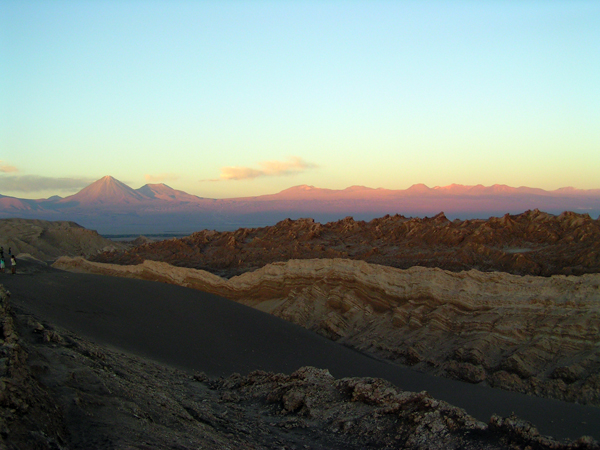
\includegraphics{valleluna.jpg}
\caption{`valleluna.jpg'}
\end{figure}

\begin{itemize}
\tightlist
\item
  L'image miroir :
\end{itemize}

\begin{figure}
\centering
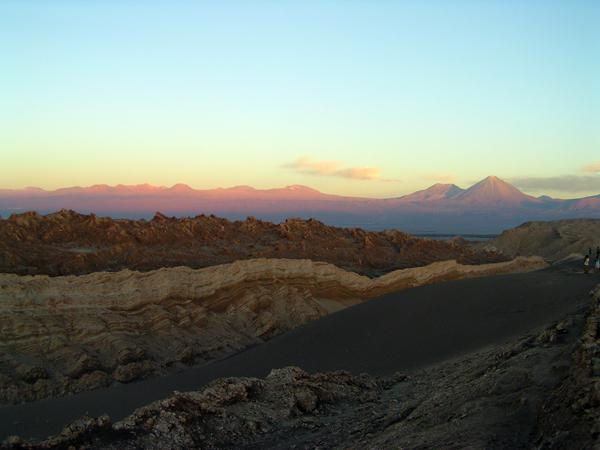
\includegraphics{miroirvalleluna.jpg}
\caption{`miroir\_valleluna.jpg'}
\end{figure}

    \hypertarget{exercice-1-passage-en-niveau-de-gris}{%
\subsection{\texorpdfstring{Exercice 1 : \emph{Passage en niveau de
gris}}{Exercice 1 : Passage en niveau de gris}}\label{exercice-1-passage-en-niveau-de-gris}}

    \begin{Verbatim}[commandchars=\\\{\}]
{\color{incolor}In [{\color{incolor}41}]:} \PY{k}{def} \PY{n+nf}{gris}\PY{p}{(}\PY{n}{imsource}\PY{p}{,} \PY{n}{coeff}\PY{p}{)}\PY{p}{:}
             \PY{l+s+sd}{\PYZdq{}\PYZdq{}\PYZdq{} coeff est une liste composée de 3 éléments \PYZdq{}\PYZdq{}\PYZdq{}}
             \PY{n}{im} \PY{o}{=} \PY{n}{Image}\PY{o}{.}\PY{n}{open}\PY{p}{(}\PY{n}{imsource}\PY{p}{)}
             \PY{n}{pixels} \PY{o}{=} \PY{n}{np}\PY{o}{.}\PY{n}{array}\PY{p}{(}\PY{n}{im}\PY{p}{)}
             \PY{n}{hauteur}\PY{p}{,} \PY{n}{largeur} \PY{o}{=} \PY{n}{pixels}\PY{o}{.}\PY{n}{shape}\PY{p}{[}\PY{p}{:}\PY{l+m+mi}{2}\PY{p}{]}
             \PY{n}{pixels\PYZus{}res} \PY{o}{=} \PY{n}{np}\PY{o}{.}\PY{n}{zeros}\PY{p}{(}\PY{p}{[}\PY{n}{hauteur}\PY{p}{,}\PY{n}{largeur}\PY{p}{]}\PY{p}{,} \PY{n}{dtype}\PY{o}{=}\PY{l+s+s2}{\PYZdq{}}\PY{l+s+s2}{uint8}\PY{l+s+s2}{\PYZdq{}}\PY{p}{)} \PY{c+c1}{\PYZsh{}pixels\PYZus{}res doit être de dimension 2}
             \PY{n}{somme\PYZus{}coef} \PY{o}{=} \PY{n}{np}\PY{o}{.}\PY{n}{sum}\PY{p}{(}\PY{n}{coeff}\PY{p}{)}
             \PY{k}{for} \PY{n}{j} \PY{o+ow}{in} \PY{n+nb}{range}\PY{p}{(}\PY{n}{largeur}\PY{p}{)}\PY{p}{:}
                 \PY{k}{for} \PY{n}{i} \PY{o+ow}{in} \PY{n+nb}{range}\PY{p}{(}\PY{n}{hauteur}\PY{p}{)}\PY{p}{:}
                     \PY{n}{pixels\PYZus{}res}\PY{p}{[}\PY{n}{i}\PY{p}{,} \PY{n}{j}\PY{p}{]} \PY{o}{=} \PY{n+nb}{int}\PY{p}{(}\PY{n}{np}\PY{o}{.}\PY{n}{sum}\PY{p}{(}\PY{n}{pixels}\PY{p}{[}\PY{n}{i}\PY{p}{,}\PY{n}{j}\PY{p}{]} \PY{o}{*} \PY{n}{coeff}\PY{p}{)}\PY{o}{/}\PY{n}{somme\PYZus{}coef}\PY{p}{)}
             \PY{n}{img\PYZus{}res} \PY{o}{=} \PY{n}{Image}\PY{o}{.}\PY{n}{fromarray}\PY{p}{(}\PY{n}{pixels\PYZus{}res}\PY{p}{)}
             \PY{n}{img\PYZus{}res}\PY{o}{.}\PY{n}{save}\PY{p}{(}\PY{l+s+s2}{\PYZdq{}}\PY{l+s+s2}{gris}\PY{l+s+s2}{\PYZdq{}}\PY{o}{+}\PY{n}{imsource}\PY{p}{)}
             \PY{n}{img\PYZus{}res}\PY{o}{.}\PY{n}{show}\PY{p}{(}\PY{p}{)} 
\end{Verbatim}


    \begin{Verbatim}[commandchars=\\\{\}]
{\color{incolor}In [{\color{incolor}42}]:} \PY{n}{gris}\PY{p}{(}\PY{l+s+s2}{\PYZdq{}}\PY{l+s+s2}{valleluna.jpg}\PY{l+s+s2}{\PYZdq{}}\PY{p}{,} \PY{p}{[}\PY{l+m+mi}{30}\PY{p}{,} \PY{l+m+mi}{59}\PY{p}{,} \PY{l+m+mi}{11}\PY{p}{]}\PY{p}{)}
\end{Verbatim}


    \begin{itemize}
\tightlist
\item
  Conversion de \texttt{valleluna.jpg} en niveaux de gris :
\end{itemize}

\begin{figure}
\centering
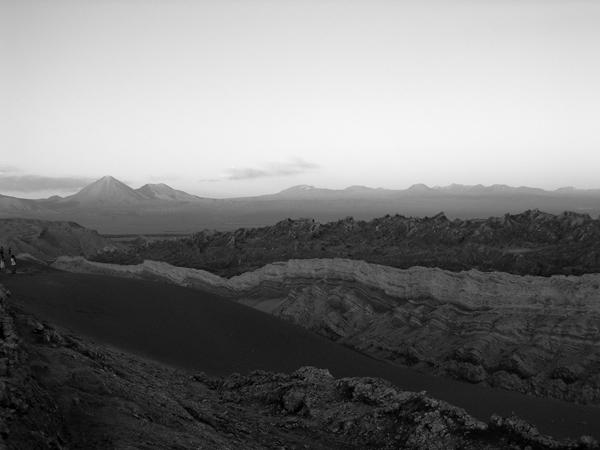
\includegraphics{grisvalleluna.jpg}
\caption{`grisvalleluna.jpg'}
\end{figure}

    \hypertarget{exercice-2-nuxe9gatif-monochrome}{%
\subsection{\texorpdfstring{Exercice 2 : \emph{Négatif /
Monochrome}}{Exercice 2 : Négatif / Monochrome}}\label{exercice-2-nuxe9gatif-monochrome}}

    \begin{Verbatim}[commandchars=\\\{\}]
{\color{incolor}In [{\color{incolor}7}]:} \PY{k}{def} \PY{n+nf}{negatif}\PY{p}{(}\PY{n}{imsource}\PY{p}{)}\PY{p}{:}
            \PY{l+s+sd}{\PYZdq{}\PYZdq{}\PYZdq{} Retourne le négatif d\PYZsq{}une image \PYZdq{}\PYZdq{}\PYZdq{}}
            \PY{n}{im} \PY{o}{=} \PY{n}{Image}\PY{o}{.}\PY{n}{open}\PY{p}{(}\PY{n}{imsource}\PY{p}{)}
            \PY{n}{pixels} \PY{o}{=} \PY{n}{np}\PY{o}{.}\PY{n}{array}\PY{p}{(}\PY{n}{im}\PY{p}{)}
            \PY{n}{pixels\PYZus{}res} \PY{o}{=} \PY{n}{np}\PY{o}{.}\PY{n}{zeros\PYZus{}like}\PY{p}{(}\PY{n}{pixels}\PY{p}{)}
            \PY{n}{pixels\PYZus{}res} \PY{o}{=} \PY{l+m+mi}{255} \PY{o}{\PYZhy{}} \PY{n}{pixels}
            \PY{n}{img\PYZus{}res} \PY{o}{=} \PY{n}{Image}\PY{o}{.}\PY{n}{fromarray}\PY{p}{(}\PY{n}{pixels\PYZus{}res}\PY{p}{)}
            \PY{n}{img\PYZus{}res}\PY{o}{.}\PY{n}{save}\PY{p}{(}\PY{l+s+s2}{\PYZdq{}}\PY{l+s+s2}{negatif}\PY{l+s+s2}{\PYZdq{}}\PY{o}{+}\PY{n}{imsource}\PY{p}{)}
            \PY{n}{img\PYZus{}res}\PY{o}{.}\PY{n}{show}\PY{p}{(}\PY{p}{)} 
            
        \PY{k}{def} \PY{n+nf}{negatif2}\PY{p}{(}\PY{n}{imsource}\PY{p}{)}\PY{p}{:}
            \PY{l+s+sd}{\PYZdq{}\PYZdq{}\PYZdq{} Retourne le négatif d\PYZsq{}une image \PYZdq{}\PYZdq{}\PYZdq{}}
            \PY{n}{im} \PY{o}{=} \PY{n}{Image}\PY{o}{.}\PY{n}{open}\PY{p}{(}\PY{n}{imsource}\PY{p}{)}
            \PY{n}{pixels} \PY{o}{=} \PY{n}{np}\PY{o}{.}\PY{n}{array}\PY{p}{(}\PY{n}{im}\PY{p}{)}
            \PY{n}{img\PYZus{}res} \PY{o}{=} \PY{n}{Image}\PY{o}{.}\PY{n}{fromarray}\PY{p}{(}\PY{l+m+mi}{255} \PY{o}{\PYZhy{}} \PY{n}{pixels}\PY{p}{)}
            \PY{n}{img\PYZus{}res}\PY{o}{.}\PY{n}{save}\PY{p}{(}\PY{l+s+s2}{\PYZdq{}}\PY{l+s+s2}{negatif}\PY{l+s+s2}{\PYZdq{}}\PY{o}{+}\PY{n}{imsource}\PY{p}{)}
            \PY{n}{img\PYZus{}res}\PY{o}{.}\PY{n}{show}\PY{p}{(}\PY{p}{)} 
\end{Verbatim}


    \begin{Verbatim}[commandchars=\\\{\}]
{\color{incolor}In [{\color{incolor}8}]:} \PY{n}{negatif}\PY{p}{(}\PY{l+s+s1}{\PYZsq{}}\PY{l+s+s1}{valleluna.jpg}\PY{l+s+s1}{\PYZsq{}}\PY{p}{)}
\end{Verbatim}


    \begin{Verbatim}[commandchars=\\\{\}]
{\color{incolor}In [{\color{incolor}40}]:} \PY{n}{negatif}\PY{p}{(}\PY{l+s+s1}{\PYZsq{}}\PY{l+s+s1}{grisvalleluna.jpg}\PY{l+s+s1}{\PYZsq{}}\PY{p}{)}
\end{Verbatim}


    \begin{itemize}
\tightlist
\item
  Le négatif de l'image \texttt{valleluna.jpg} :
\end{itemize}

\begin{figure}
\centering
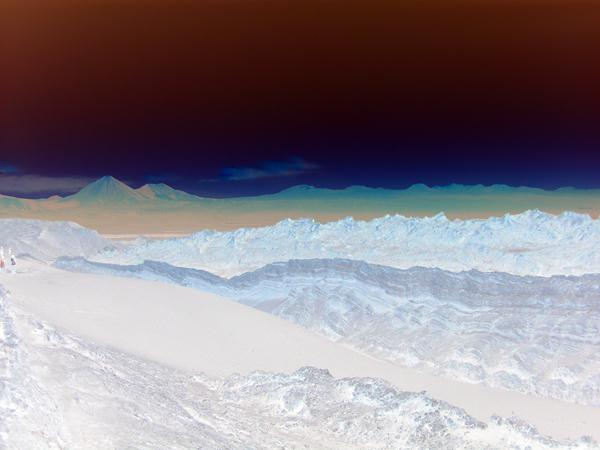
\includegraphics{negatifvalleluna.jpg}
\caption{`negatifvalleluna.jpg'}
\end{figure}

\begin{itemize}
\tightlist
\item
  Le négatif de l'image en niveaux de gris \texttt{grisvalleluna.jpg} :
\end{itemize}

\begin{figure}
\centering
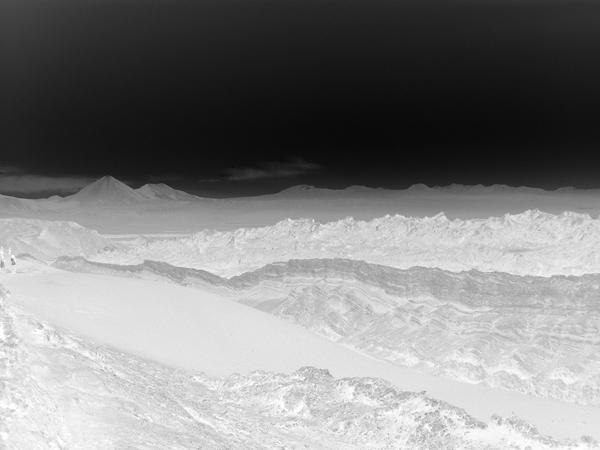
\includegraphics{negatifgrisvalleluna.jpg}
\caption{`negatifvalleluna.jpg'}
\end{figure}

    \hypertarget{exercice-3-extraction-de-composantes}{%
\subsection{\texorpdfstring{Exercice 3 \emph{Extraction de
composantes}}{Exercice 3 Extraction de composantes}}\label{exercice-3-extraction-de-composantes}}

    \begin{Verbatim}[commandchars=\\\{\}]
{\color{incolor}In [{\color{incolor}126}]:} \PY{k}{def} \PY{n+nf}{monochrome}\PY{p}{(}\PY{n}{imsource}\PY{p}{)}\PY{p}{:}
              \PY{l+s+sd}{\PYZdq{}\PYZdq{}\PYZdq{}prend en entrée un fichier image et retourne une version monochome pour chacune des couleurs}
          \PY{l+s+sd}{    \PYZdq{}\PYZdq{}\PYZdq{}}
              \PY{n}{im}\PY{o}{=}\PY{n}{Image}\PY{o}{.}\PY{n}{open}\PY{p}{(}\PY{n}{imsource}\PY{p}{)}
              \PY{n}{pixels} \PY{o}{=} \PY{n}{np}\PY{o}{.}\PY{n}{array}\PY{p}{(}\PY{n}{im}\PY{p}{)}
              \PY{n}{hauteur}\PY{p}{,} \PY{n}{largeur} \PY{o}{=}\PY{n}{pixels}\PY{o}{.}\PY{n}{shape}\PY{p}{[}\PY{p}{:}\PY{l+m+mi}{2}\PY{p}{]}
              \PY{n}{pixels\PYZus{}res\PYZus{}rouge} \PY{o}{=} \PY{n}{np}\PY{o}{.}\PY{n}{zeros\PYZus{}like}\PY{p}{(}\PY{n}{pixels}\PY{p}{)}
              \PY{n}{pixels\PYZus{}res\PYZus{}vert} \PY{o}{=} \PY{n}{np}\PY{o}{.}\PY{n}{zeros\PYZus{}like}\PY{p}{(}\PY{n}{pixels}\PY{p}{)}
              \PY{n}{pixels\PYZus{}res\PYZus{}bleu} \PY{o}{=} \PY{n}{np}\PY{o}{.}\PY{n}{zeros\PYZus{}like}\PY{p}{(}\PY{n}{pixels}\PY{p}{)}
              \PY{k}{for} \PY{n}{i} \PY{o+ow}{in} \PY{n+nb}{range}\PY{p}{(}\PY{n}{hauteur}\PY{p}{)}\PY{p}{:}
                  \PY{k}{for} \PY{n}{j} \PY{o+ow}{in} \PY{n+nb}{range}\PY{p}{(}\PY{n}{largeur}\PY{p}{)}\PY{p}{:}
                      \PY{p}{[}\PY{n}{r}\PY{p}{,} \PY{n}{g}\PY{p}{,} \PY{n}{b}\PY{p}{]} \PY{o}{=} \PY{n}{pixels}\PY{p}{[}\PY{n}{i}\PY{p}{,}\PY{n}{j}\PY{p}{,}\PY{p}{:}\PY{p}{]}
                      \PY{n}{pixels\PYZus{}res\PYZus{}rouge}\PY{p}{[}\PY{n}{i}\PY{p}{,} \PY{n}{j}\PY{p}{]} \PY{o}{=} \PY{p}{[}\PY{n}{r}\PY{p}{,} \PY{l+m+mi}{0}\PY{p}{,} \PY{l+m+mi}{0}\PY{p}{]}
                      \PY{n}{pixels\PYZus{}res\PYZus{}vert}\PY{p}{[}\PY{n}{i}\PY{p}{,} \PY{n}{j}\PY{p}{]} \PY{o}{=} \PY{p}{[}\PY{l+m+mi}{0}\PY{p}{,} \PY{n}{g}\PY{p}{,} \PY{l+m+mi}{0}\PY{p}{]}
                      \PY{n}{pixels\PYZus{}res\PYZus{}bleu}\PY{p}{[}\PY{n}{i}\PY{p}{,} \PY{n}{j}\PY{p}{]} \PY{o}{=} \PY{p}{[}\PY{l+m+mi}{0}\PY{p}{,} \PY{l+m+mi}{0}\PY{p}{,} \PY{n}{b}\PY{p}{]}
              \PY{n}{img\PYZus{}res\PYZus{}r} \PY{o}{=} \PY{n}{Image}\PY{o}{.}\PY{n}{fromarray}\PY{p}{(}\PY{n}{pixels\PYZus{}res\PYZus{}rouge}\PY{p}{)}
              \PY{n}{img\PYZus{}res\PYZus{}r}\PY{o}{.}\PY{n}{save}\PY{p}{(}\PY{l+s+s2}{\PYZdq{}}\PY{l+s+s2}{rouge}\PY{l+s+s2}{\PYZdq{}}\PY{o}{+}\PY{n}{imsource}\PY{p}{)}
              \PY{n}{img\PYZus{}res\PYZus{}r}\PY{o}{.}\PY{n}{show}\PY{p}{(}\PY{p}{)}
              \PY{n}{img\PYZus{}res\PYZus{}v} \PY{o}{=} \PY{n}{Image}\PY{o}{.}\PY{n}{fromarray}\PY{p}{(}\PY{n}{pixels\PYZus{}res\PYZus{}vert}\PY{p}{)}
              \PY{n}{img\PYZus{}res\PYZus{}v}\PY{o}{.}\PY{n}{save}\PY{p}{(}\PY{l+s+s2}{\PYZdq{}}\PY{l+s+s2}{vert}\PY{l+s+s2}{\PYZdq{}}\PY{o}{+}\PY{n}{imsource}\PY{p}{)}
              \PY{n}{img\PYZus{}res\PYZus{}v}\PY{o}{.}\PY{n}{show}\PY{p}{(}\PY{p}{)}
              \PY{n}{img\PYZus{}res\PYZus{}b} \PY{o}{=} \PY{n}{Image}\PY{o}{.}\PY{n}{fromarray}\PY{p}{(}\PY{n}{pixels\PYZus{}res\PYZus{}bleu}\PY{p}{)}
              \PY{n}{img\PYZus{}res\PYZus{}b}\PY{o}{.}\PY{n}{save}\PY{p}{(}\PY{l+s+s2}{\PYZdq{}}\PY{l+s+s2}{bleu}\PY{l+s+s2}{\PYZdq{}}\PY{o}{+}\PY{n}{imsource}\PY{p}{)}
              \PY{n}{img\PYZus{}res\PYZus{}b}\PY{o}{.}\PY{n}{show}\PY{p}{(}\PY{p}{)}  
              
          \PY{k}{def} \PY{n+nf}{monochrome\PYZus{}slicing}\PY{p}{(}\PY{n}{imsource}\PY{p}{)}\PY{p}{:}
              \PY{l+s+sd}{\PYZdq{}\PYZdq{}\PYZdq{}prend en entrée un fichier image et retourne une version monochome pour chacune des couleurs}
          \PY{l+s+sd}{    \PYZdq{}\PYZdq{}\PYZdq{}}
              \PY{n}{im}\PY{o}{=}\PY{n}{Image}\PY{o}{.}\PY{n}{open}\PY{p}{(}\PY{n}{imsource}\PY{p}{)}
              \PY{n}{pixels} \PY{o}{=} \PY{n}{np}\PY{o}{.}\PY{n}{array}\PY{p}{(}\PY{n}{im}\PY{p}{)}
              \PY{n}{pixels\PYZus{}res\PYZus{}rouge} \PY{o}{=} \PY{n}{np}\PY{o}{.}\PY{n}{zeros\PYZus{}like}\PY{p}{(}\PY{n}{pixels}\PY{p}{)}
              \PY{n}{pixels\PYZus{}res\PYZus{}rouge}\PY{p}{[}\PY{p}{:}\PY{p}{,}\PY{p}{:}\PY{p}{,}\PY{l+m+mi}{0}\PY{p}{]} \PY{o}{=} \PY{n}{pixels}\PY{p}{[}\PY{p}{:}\PY{p}{,}\PY{p}{:}\PY{p}{,}\PY{l+m+mi}{0}\PY{p}{]} 
              \PY{n}{pixels\PYZus{}res\PYZus{}vert} \PY{o}{=} \PY{n}{np}\PY{o}{.}\PY{n}{zeros\PYZus{}like}\PY{p}{(}\PY{n}{pixels}\PY{p}{)}
              \PY{n}{pixels\PYZus{}res\PYZus{}vert}\PY{p}{[}\PY{p}{:}\PY{p}{,}\PY{p}{:}\PY{p}{,}\PY{l+m+mi}{1}\PY{p}{]} \PY{o}{=} \PY{n}{pixels}\PY{p}{[}\PY{p}{:}\PY{p}{,}\PY{p}{:}\PY{p}{,}\PY{l+m+mi}{1}\PY{p}{]} 
              \PY{n}{pixels\PYZus{}res\PYZus{}bleu} \PY{o}{=} \PY{n}{np}\PY{o}{.}\PY{n}{zeros\PYZus{}like}\PY{p}{(}\PY{n}{pixels}\PY{p}{)}
              \PY{n}{pixels\PYZus{}res\PYZus{}bleu}\PY{p}{[}\PY{p}{:}\PY{p}{,}\PY{p}{:}\PY{p}{,}\PY{l+m+mi}{2}\PY{p}{]} \PY{o}{=} \PY{n}{pixels}\PY{p}{[}\PY{p}{:}\PY{p}{,}\PY{p}{:}\PY{p}{,}\PY{l+m+mi}{2}\PY{p}{]} 
              \PY{n}{img\PYZus{}res\PYZus{}r} \PY{o}{=} \PY{n}{Image}\PY{o}{.}\PY{n}{fromarray}\PY{p}{(}\PY{n}{pixels\PYZus{}res\PYZus{}rouge}\PY{p}{)}
              \PY{n}{img\PYZus{}res\PYZus{}r}\PY{o}{.}\PY{n}{save}\PY{p}{(}\PY{l+s+s2}{\PYZdq{}}\PY{l+s+s2}{rouge}\PY{l+s+s2}{\PYZdq{}}\PY{o}{+}\PY{n}{imsource}\PY{p}{)}
              \PY{n}{img\PYZus{}res\PYZus{}r}\PY{o}{.}\PY{n}{show}\PY{p}{(}\PY{p}{)}
              \PY{n}{img\PYZus{}res\PYZus{}v} \PY{o}{=} \PY{n}{Image}\PY{o}{.}\PY{n}{fromarray}\PY{p}{(}\PY{n}{pixels\PYZus{}res\PYZus{}vert}\PY{p}{)}
              \PY{n}{img\PYZus{}res\PYZus{}v}\PY{o}{.}\PY{n}{save}\PY{p}{(}\PY{l+s+s2}{\PYZdq{}}\PY{l+s+s2}{vert}\PY{l+s+s2}{\PYZdq{}}\PY{o}{+}\PY{n}{imsource}\PY{p}{)}
              \PY{n}{img\PYZus{}res\PYZus{}v}\PY{o}{.}\PY{n}{show}\PY{p}{(}\PY{p}{)}
              \PY{n}{img\PYZus{}res\PYZus{}b} \PY{o}{=} \PY{n}{Image}\PY{o}{.}\PY{n}{fromarray}\PY{p}{(}\PY{n}{pixels\PYZus{}res\PYZus{}bleu}\PY{p}{)}
              \PY{n}{img\PYZus{}res\PYZus{}b}\PY{o}{.}\PY{n}{save}\PY{p}{(}\PY{l+s+s2}{\PYZdq{}}\PY{l+s+s2}{bleu}\PY{l+s+s2}{\PYZdq{}}\PY{o}{+}\PY{n}{imsource}\PY{p}{)}
              \PY{n}{img\PYZus{}res\PYZus{}b}\PY{o}{.}\PY{n}{show}\PY{p}{(}\PY{p}{)}
\end{Verbatim}


    \begin{Verbatim}[commandchars=\\\{\}]
{\color{incolor}In [{\color{incolor}61}]:} \PY{n}{monochrome\PYZus{}slicing}\PY{p}{(}\PY{l+s+s1}{\PYZsq{}}\PY{l+s+s1}{valleluna.jpg}\PY{l+s+s1}{\PYZsq{}}\PY{p}{)}
\end{Verbatim}


    \begin{itemize}
\tightlist
\item
  Composante rouge de \texttt{valleluna.jpg} :
\end{itemize}

\begin{figure}
\centering
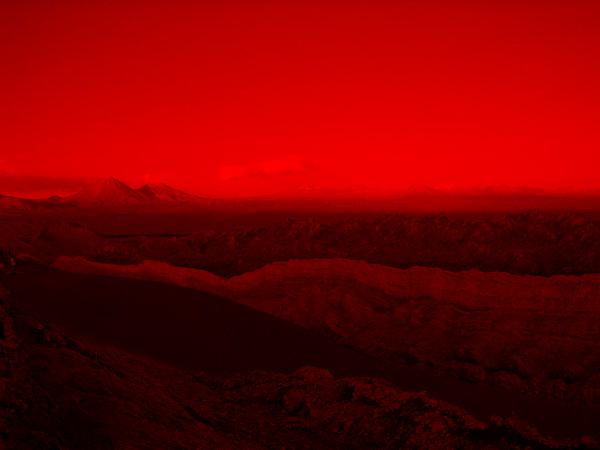
\includegraphics{rougevalleluna.jpg}
\caption{``rougevalleluna.jpg''}
\end{figure}

\begin{itemize}
\tightlist
\item
  Composante verte de \texttt{valleluna.jpg} :
\end{itemize}

\begin{figure}
\centering
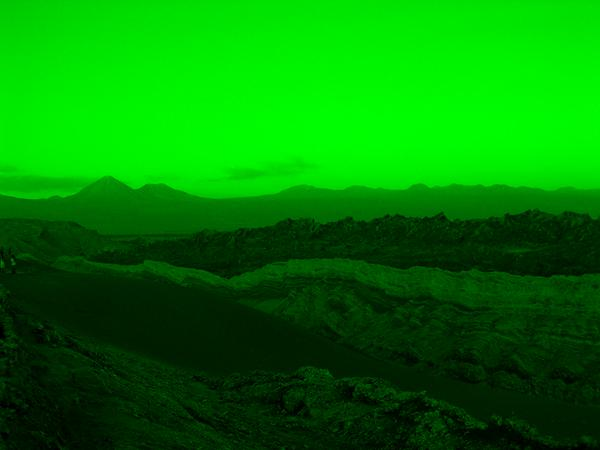
\includegraphics{vertvalleluna.jpg}
\caption{``vertvalleluna.jpg''}
\end{figure}

\begin{itemize}
\tightlist
\item
  Composante bleue de \texttt{valleluna.jpg} :
\end{itemize}

\begin{figure}
\centering
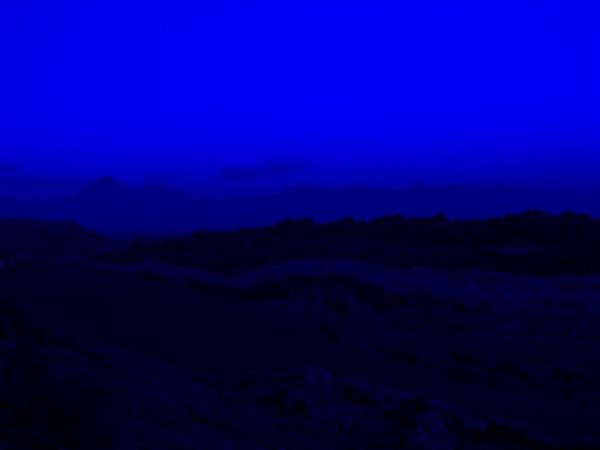
\includegraphics{bleuvalleluna.jpg}
\caption{``bleuvalleluna.jpg''}
\end{figure}

    \hypertarget{exercice-4-maxmin}{%
\subsection{\texorpdfstring{Exercice 4
\emph{Max/Min}}{Exercice 4 Max/Min}}\label{exercice-4-maxmin}}

    \begin{Verbatim}[commandchars=\\\{\}]
{\color{incolor}In [{\color{incolor}1}]:} \PY{k}{def} \PY{n+nf}{maxmin}\PY{p}{(}\PY{n}{x}\PY{p}{)}\PY{p}{:}
            \PY{l+s+sd}{\PYZdq{}\PYZdq{}\PYZdq{}Retourne 0 si x \PYZlt{} 255, 255 si x \PYZgt{} 255 et x sinon\PYZdq{}\PYZdq{}\PYZdq{}}
            \PY{k}{return} \PY{n+nb}{int}\PY{p}{(}\PY{n+nb}{max}\PY{p}{(}\PY{n+nb}{min}\PY{p}{(}\PY{n}{x}\PY{p}{,} \PY{l+m+mi}{255}\PY{p}{)}\PY{p}{,} \PY{l+m+mi}{0}\PY{p}{)}\PY{p}{)}
        
        \PY{k}{def} \PY{n+nf}{maxmin2}\PY{p}{(}\PY{n}{x}\PY{p}{)}\PY{p}{:}
            \PY{l+s+sd}{\PYZdq{}\PYZdq{}\PYZdq{}Retourne 0 si x \PYZlt{} 255, 255 si x \PYZgt{} 255 et x sinon\PYZdq{}\PYZdq{}\PYZdq{}}
            \PY{k}{return} \PY{n+nb}{int}\PY{p}{(}\PY{n+nb}{min}\PY{p}{(}\PY{n+nb}{max}\PY{p}{(}\PY{n}{x}\PY{p}{,} \PY{l+m+mi}{0}\PY{p}{)}\PY{p}{,} \PY{l+m+mi}{255}\PY{p}{)}\PY{p}{)}
\end{Verbatim}


    \begin{Verbatim}[commandchars=\\\{\}]
{\color{incolor}In [{\color{incolor}64}]:} \PY{p}{[}\PY{n}{maxmin}\PY{p}{(}\PY{n}{x}\PY{p}{)} \PY{k}{for} \PY{n}{x} \PY{o+ow}{in} \PY{p}{[}\PY{o}{\PYZhy{}}\PY{l+m+mi}{10}\PY{p}{,} \PY{l+m+mi}{0}\PY{p}{,} \PY{l+m+mi}{128}\PY{p}{,} \PY{l+m+mi}{255}\PY{p}{,} \PY{l+m+mi}{256}\PY{p}{]}\PY{p}{]}
\end{Verbatim}


\begin{Verbatim}[commandchars=\\\{\}]
{\color{outcolor}Out[{\color{outcolor}64}]:} [0, 0, 128, 255, 255]
\end{Verbatim}
            
    \begin{Verbatim}[commandchars=\\\{\}]
{\color{incolor}In [{\color{incolor}68}]:} \PY{n}{les\PYZus{}x} \PY{o}{=} \PY{n}{np}\PY{o}{.}\PY{n}{arange}\PY{p}{(}\PY{o}{\PYZhy{}}\PY{l+m+mi}{250}\PY{p}{,} \PY{l+m+mi}{500}\PY{p}{,}\PY{l+m+mi}{1}\PY{p}{)}
         \PY{n}{plt}\PY{o}{.}\PY{n}{plot}\PY{p}{(}\PY{n}{les\PYZus{}x}\PY{p}{,} \PY{p}{[}\PY{n}{maxmin}\PY{p}{(}\PY{n}{v}\PY{p}{)} \PY{k}{for} \PY{n}{v} \PY{o+ow}{in} \PY{n}{les\PYZus{}x}\PY{p}{]}\PY{p}{)}
\end{Verbatim}


\begin{Verbatim}[commandchars=\\\{\}]
{\color{outcolor}Out[{\color{outcolor}68}]:} [<matplotlib.lines.Line2D at 0x7f4318d28828>]
\end{Verbatim}
            
    \begin{center}
    \adjustimage{max size={0.9\linewidth}{0.9\paperheight}}{output_25_1.png}
    \end{center}
    { \hspace*{\fill} \\}
    
    \begin{Verbatim}[commandchars=\\\{\}]
{\color{incolor}In [{\color{incolor}51}]:} \PY{k}{def} \PY{n+nf}{maxminmat}\PY{p}{(}\PY{n}{matrice}\PY{p}{)}\PY{p}{:}
             \PY{n}{taille}\PY{o}{=}\PY{n}{matrice}\PY{o}{.}\PY{n}{shape}
             \PY{n}{res}\PY{o}{=}\PY{n}{np}\PY{o}{.}\PY{n}{zeros\PYZus{}like}\PY{p}{(}\PY{n}{matrice}\PY{p}{)}
             \PY{k}{if} \PY{n+nb}{len}\PY{p}{(}\PY{n}{taille}\PY{p}{)}\PY{o}{==}\PY{l+m+mi}{3}\PY{p}{:}
                 \PY{k}{for} \PY{n}{i} \PY{o+ow}{in} \PY{n+nb}{range}\PY{p}{(}\PY{n}{taille}\PY{p}{[}\PY{l+m+mi}{0}\PY{p}{]}\PY{p}{)}\PY{p}{:}
                     \PY{k}{for} \PY{n}{j} \PY{o+ow}{in} \PY{n+nb}{range}\PY{p}{(}\PY{n}{taille}\PY{p}{[}\PY{l+m+mi}{1}\PY{p}{]}\PY{p}{)}\PY{p}{:}
                         \PY{k}{for} \PY{n}{k} \PY{o+ow}{in} \PY{n+nb}{range}\PY{p}{(}\PY{n}{taille}\PY{p}{[}\PY{l+m+mi}{2}\PY{p}{]}\PY{p}{)}\PY{p}{:}
                             \PY{n}{res}\PY{p}{[}\PY{n}{i}\PY{p}{,}\PY{n}{j}\PY{p}{,}\PY{n}{k}\PY{p}{]}\PY{o}{=}\PY{n}{maxmin}\PY{p}{(}\PY{n}{matrice}\PY{p}{[}\PY{n}{i}\PY{p}{,}\PY{n}{j}\PY{p}{,}\PY{n}{k}\PY{p}{]}\PY{p}{)}
             \PY{k}{else}\PY{p}{:}
                 \PY{k}{for} \PY{n}{i} \PY{o+ow}{in} \PY{n+nb}{range}\PY{p}{(}\PY{n}{taille}\PY{p}{[}\PY{l+m+mi}{0}\PY{p}{]}\PY{p}{)}\PY{p}{:}
                     \PY{k}{for} \PY{n}{j} \PY{o+ow}{in} \PY{n+nb}{range}\PY{p}{(}\PY{n}{taille}\PY{p}{[}\PY{l+m+mi}{1}\PY{p}{]}\PY{p}{)}\PY{p}{:}
                         \PY{n}{res}\PY{p}{[}\PY{n}{i}\PY{p}{,}\PY{n}{j}\PY{p}{]}\PY{o}{=}\PY{n}{maxmin}\PY{p}{(}\PY{n}{matrice}\PY{p}{[}\PY{n}{i}\PY{p}{,}\PY{n}{j}\PY{p}{]}\PY{p}{)}
             \PY{k}{return} \PY{n}{res}
         
         \PY{k}{def} \PY{n+nf}{maxminmatV2}\PY{p}{(}\PY{n}{matrice}\PY{p}{)}\PY{p}{:}
             \PY{n}{hauteur}\PY{p}{,} \PY{n}{largeur} \PY{o}{=} \PY{n}{matrice}\PY{o}{.}\PY{n}{shape}\PY{p}{[}\PY{p}{:}\PY{l+m+mi}{2}\PY{p}{]}
             \PY{k}{if} \PY{n+nb}{len}\PY{p}{(}\PY{n}{matrice}\PY{o}{.}\PY{n}{shape}\PY{p}{)} \PY{o}{==} \PY{l+m+mi}{2}\PY{p}{:}        
                 \PY{k}{return} \PY{n}{np}\PY{o}{.}\PY{n}{array}\PY{p}{(}\PY{p}{[}\PY{p}{[}\PY{n}{maxmin}\PY{p}{(}\PY{n}{matrice}\PY{p}{[}\PY{n}{i}\PY{p}{,}\PY{n}{j}\PY{p}{]}\PY{p}{)}   \PY{k}{for} \PY{n}{j} \PY{o+ow}{in} \PY{n+nb}{range}\PY{p}{(}\PY{n}{largeur}\PY{p}{)}\PY{p}{]} \PY{k}{for} \PY{n}{i} \PY{o+ow}{in} \PY{n+nb}{range}\PY{p}{(}\PY{n}{hauteur}\PY{p}{)}\PY{p}{]}\PY{p}{)}
             \PY{k}{elif} \PY{n+nb}{len}\PY{p}{(}\PY{n}{matrice}\PY{o}{.}\PY{n}{shape}\PY{p}{)} \PY{o}{==} \PY{l+m+mi}{3}\PY{p}{:}
                 \PY{k}{return} \PY{n}{np}\PY{o}{.}\PY{n}{array}\PY{p}{(}\PY{p}{[}\PY{p}{[}\PY{p}{[}\PY{n}{maxmin}\PY{p}{(}\PY{n}{matrice}\PY{p}{[}\PY{n}{i}\PY{p}{,}\PY{n}{j}\PY{p}{,}\PY{n}{k}\PY{p}{]}\PY{p}{)} \PY{k}{for} \PY{n}{k} \PY{o+ow}{in} \PY{n+nb}{range}\PY{p}{(}\PY{n}{matrice}\PY{o}{.}\PY{n}{shape}\PY{p}{[}\PY{l+m+mi}{2}\PY{p}{]}\PY{p}{)}\PY{p}{]}  \PY{k}{for} \PY{n}{j} \PY{o+ow}{in} \PY{n+nb}{range}\PY{p}{(}\PY{n}{largeur}\PY{p}{)}\PY{p}{]} \PY{k}{for} \PY{n}{i} \PY{o+ow}{in} \PY{n+nb}{range}\PY{p}{(}\PY{n}{hauteur}\PY{p}{)}\PY{p}{]}\PY{p}{)}
\end{Verbatim}


    \begin{Verbatim}[commandchars=\\\{\}]
{\color{incolor}In [{\color{incolor}83}]:} \PY{n}{mtest} \PY{o}{=} \PY{n}{np}\PY{o}{.}\PY{n}{random}\PY{o}{.}\PY{n}{randint}\PY{p}{(}\PY{o}{\PYZhy{}}\PY{l+m+mi}{500}\PY{p}{,}\PY{l+m+mi}{500}\PY{p}{,}\PY{p}{(}\PY{l+m+mi}{4}\PY{p}{,}\PY{l+m+mi}{4}\PY{p}{)}\PY{p}{)}
         \PY{n}{mtest}
\end{Verbatim}


\begin{Verbatim}[commandchars=\\\{\}]
{\color{outcolor}Out[{\color{outcolor}83}]:} array([[-475, -219, -274, -459],
                [-231,   65,  419,  183],
                [ 156,   54,  220,    2],
                [ 173,  165,  465,   27]])
\end{Verbatim}
            
    \begin{Verbatim}[commandchars=\\\{\}]
{\color{incolor}In [{\color{incolor}87}]:} \PY{n}{maxminmat}\PY{p}{(}\PY{n}{mtest}\PY{p}{)}
\end{Verbatim}


\begin{Verbatim}[commandchars=\\\{\}]
{\color{outcolor}Out[{\color{outcolor}87}]:} array([[  0,   0,   0,   0],
                [  0,  65, 255, 183],
                [156,  54, 220,   2],
                [173, 165, 255,  27]])
\end{Verbatim}
            
    \begin{Verbatim}[commandchars=\\\{\}]
{\color{incolor}In [{\color{incolor}88}]:} \PY{n}{maxminmatV2}\PY{p}{(}\PY{n}{mtest}\PY{p}{)}
\end{Verbatim}


\begin{Verbatim}[commandchars=\\\{\}]
{\color{outcolor}Out[{\color{outcolor}88}]:} array([[  0,   0,   0,   0],
                [  0,  65, 255, 183],
                [156,  54, 220,   2],
                [173, 165, 255,  27]])
\end{Verbatim}
            
    \hypertarget{exercice-5-luminosituxe9-1}{%
\subsection{Exercice 5 Luminosité 1}\label{exercice-5-luminosituxe9-1}}

    \begin{Verbatim}[commandchars=\\\{\}]
{\color{incolor}In [{\color{incolor}50}]:} \PY{k}{def} \PY{n+nf}{luminosite1}\PY{p}{(}\PY{n}{imsource}\PY{p}{,}\PY{n}{unite}\PY{p}{)}\PY{p}{:}
             \PY{n}{im} \PY{o}{=} \PY{n}{Image}\PY{o}{.}\PY{n}{open}\PY{p}{(}\PY{n}{imsource}\PY{p}{)}
             \PY{n}{pixels} \PY{o}{=} \PY{n}{np}\PY{o}{.}\PY{n}{array}\PY{p}{(}\PY{n}{im}\PY{p}{)}
             \PY{c+c1}{\PYZsh{}pour ne plus calculer modulo 255 avec des entiers sur 8 bits}
             \PY{n}{pixels} \PY{o}{=} \PY{n}{pixels}\PY{o}{.}\PY{n}{astype}\PY{p}{(}\PY{n+nb}{int}\PY{p}{)}  
             \PY{c+c1}{\PYZsh{}seuillage}
             \PY{n}{pixels\PYZus{}res} \PY{o}{=} \PY{n}{maxminmat}\PY{p}{(}\PY{n}{pixels}\PY{o}{+}\PY{n}{unite}\PY{p}{)}
             \PY{c+c1}{\PYZsh{}on revient dans la plage modulo 255 avec des entiers sur 8 bits}
             \PY{n}{pixels\PYZus{}res} \PY{o}{=} \PY{n}{pixels\PYZus{}res}\PY{o}{.}\PY{n}{astype}\PY{p}{(}\PY{n}{np}\PY{o}{.}\PY{n}{uint8}\PY{p}{)}
             \PY{n}{img\PYZus{}res} \PY{o}{=} \PY{n}{Image}\PY{o}{.}\PY{n}{fromarray}\PY{p}{(}\PY{n}{pixels\PYZus{}res}\PY{p}{)}
             \PY{n}{img\PYZus{}res}\PY{o}{.}\PY{n}{save}\PY{p}{(}\PY{l+s+s2}{\PYZdq{}}\PY{l+s+s2}{lum1\PYZus{}}\PY{l+s+s2}{\PYZdq{}}\PY{o}{+}\PY{n}{imsource}\PY{p}{)}
             \PY{n}{img\PYZus{}res}\PY{o}{.}\PY{n}{show}\PY{p}{(}\PY{p}{)}    
\end{Verbatim}


    \begin{Verbatim}[commandchars=\\\{\}]
{\color{incolor}In [{\color{incolor}18}]:} \PY{n}{luminosite1}\PY{p}{(}\PY{l+s+s1}{\PYZsq{}}\PY{l+s+s1}{valleluna.jpg}\PY{l+s+s1}{\PYZsq{}}\PY{p}{,} \PY{l+m+mi}{50}\PY{p}{)}
\end{Verbatim}


    \begin{itemize}
\tightlist
\item
  Image \texttt{valleluna.jpg} éclaircie de 50 pixels :
\end{itemize}

\begin{figure}
\centering
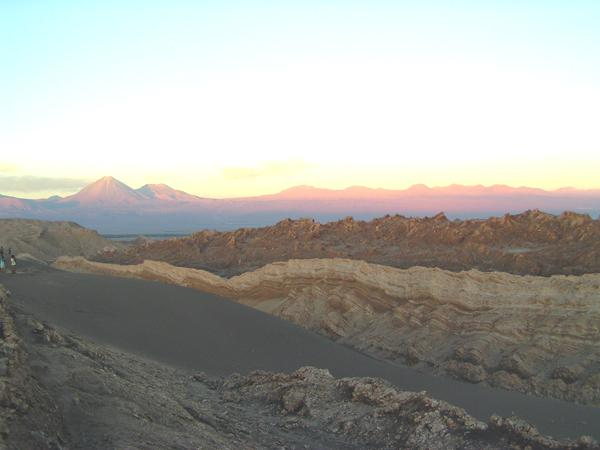
\includegraphics{lum1_valleluna.jpg}
\caption{`lum1\_valleluna.jpg'}
\end{figure}

    \hypertarget{exercice-6-luminosituxe9-contraste}{%
\subsection{\texorpdfstring{Exercice 6 \emph{Luminosité,
contraste}}{Exercice 6 Luminosité, contraste}}\label{exercice-6-luminosituxe9-contraste}}

    \begin{Verbatim}[commandchars=\\\{\}]
{\color{incolor}In [{\color{incolor}49}]:} \PY{c+c1}{\PYZsh{} Liste des fonctions}
         
         \PY{k}{def} \PY{n+nf}{filtre\PYZus{}puissance}\PY{p}{(}\PY{n}{x}\PY{p}{,}\PY{n}{p}\PY{p}{)}\PY{p}{:}
             \PY{k}{return} \PY{n+nb}{int}\PY{p}{(}\PY{l+m+mi}{255}\PY{o}{*}\PY{p}{(}\PY{n}{x}\PY{o}{/}\PY{l+m+mi}{255}\PY{p}{)}\PY{o}{*}\PY{o}{*}\PY{n}{p}\PY{p}{)}
             
         \PY{k}{def} \PY{n+nf}{f}\PY{p}{(}\PY{n}{x}\PY{p}{)}\PY{p}{:}
             \PY{k}{return} \PY{l+m+mi}{3}\PY{o}{*}\PY{n}{x}\PY{o}{*}\PY{o}{*}\PY{l+m+mi}{2}\PY{o}{\PYZhy{}}\PY{l+m+mi}{2}\PY{o}{*}\PY{n}{x}\PY{o}{*}\PY{o}{*}\PY{l+m+mi}{3}
             
         \PY{k}{def} \PY{n+nf}{g}\PY{p}{(}\PY{n}{x}\PY{p}{)}\PY{p}{:}
             \PY{k}{return} \PY{p}{(}\PY{n}{x}\PY{o}{*}\PY{o}{*}\PY{l+m+mi}{3}\PY{p}{)}\PY{o}{*}\PY{p}{(}\PY{l+m+mi}{6}\PY{o}{*}\PY{n}{x}\PY{o}{*}\PY{o}{*}\PY{l+m+mi}{2} \PY{o}{\PYZhy{}}\PY{l+m+mi}{15}\PY{o}{*}\PY{n}{x} \PY{o}{+} \PY{l+m+mi}{10}\PY{p}{)}
         
         \PY{k}{def} \PY{n+nf}{filtre\PYZus{}f}\PY{p}{(}\PY{n}{x}\PY{p}{,} \PY{n}{p}\PY{p}{)}\PY{p}{:}
             \PY{k}{return} \PY{n+nb}{int}\PY{p}{(}\PY{l+m+mi}{255}\PY{o}{*}\PY{n}{f}\PY{p}{(}\PY{n}{x}\PY{o}{/}\PY{l+m+mi}{255}\PY{p}{)}\PY{p}{)}
         
         \PY{k}{def} \PY{n+nf}{filtre\PYZus{}g}\PY{p}{(}\PY{n}{x}\PY{p}{,} \PY{n}{p}\PY{p}{)}\PY{p}{:}
             \PY{k}{return} \PY{n+nb}{int}\PY{p}{(}\PY{l+m+mi}{255}\PY{o}{*}\PY{n}{g}\PY{p}{(}\PY{n}{x}\PY{o}{/}\PY{l+m+mi}{255}\PY{p}{)}\PY{p}{)}
         
         \PY{c+c1}{\PYZsh{} Fonction lum\PYZus{}contraste}
         
         \PY{k}{def} \PY{n+nf}{lum\PYZus{}contraste}\PY{p}{(}\PY{n}{imsource}\PY{p}{,}\PY{n}{fonction}\PY{p}{,}\PY{n}{parametre}\PY{p}{)}\PY{p}{:}
             \PY{n}{im}\PY{o}{=}\PY{n}{Image}\PY{o}{.}\PY{n}{open}\PY{p}{(}\PY{n}{imsource}\PY{p}{)}
             \PY{n}{pixels} \PY{o}{=} \PY{n}{np}\PY{o}{.}\PY{n}{array}\PY{p}{(}\PY{n}{im}\PY{p}{)}
             \PY{n}{hauteur}\PY{p}{,} \PY{n}{largeur} \PY{o}{=} \PY{n}{pixels}\PY{o}{.}\PY{n}{shape}\PY{p}{[}\PY{p}{:}\PY{l+m+mi}{2}\PY{p}{]}
             \PY{n}{pixels\PYZus{}res} \PY{o}{=} \PY{n}{np}\PY{o}{.}\PY{n}{zeros\PYZus{}like}\PY{p}{(}\PY{n}{pixels}\PY{p}{)}
             \PY{k}{if} \PY{n+nb}{len}\PY{p}{(}\PY{n}{pixels}\PY{o}{.}\PY{n}{shape}\PY{p}{)} \PY{o}{==} \PY{l+m+mi}{3}\PY{p}{:}
                 \PY{k}{for} \PY{n}{i} \PY{o+ow}{in} \PY{n+nb}{range}\PY{p}{(}\PY{n}{hauteur}\PY{p}{)}\PY{p}{:}
                     \PY{k}{for} \PY{n}{j} \PY{o+ow}{in} \PY{n+nb}{range}\PY{p}{(}\PY{n}{largeur}\PY{p}{)}\PY{p}{:}
                         \PY{k}{for} \PY{n}{k} \PY{o+ow}{in} \PY{n+nb}{range}\PY{p}{(}\PY{l+m+mi}{3}\PY{p}{)}\PY{p}{:}
                             \PY{n}{pixels\PYZus{}res}\PY{p}{[}\PY{n}{i}\PY{p}{,}\PY{n}{j}\PY{p}{,}\PY{n}{k}\PY{p}{]} \PY{o}{=} \PY{n}{maxmin}\PY{p}{(}\PY{n}{fonction}\PY{p}{(}\PY{n}{pixels}\PY{p}{[}\PY{n}{i}\PY{p}{,}\PY{n}{j}\PY{p}{,}\PY{n}{k}\PY{p}{]}\PY{p}{,}\PY{n}{parametre}\PY{p}{)}\PY{p}{)}
             \PY{k}{else}\PY{p}{:}
                 \PY{k}{for} \PY{n}{i} \PY{o+ow}{in} \PY{n+nb}{range}\PY{p}{(}\PY{n}{hauteur}\PY{p}{)}\PY{p}{:}
                     \PY{k}{for} \PY{n}{j} \PY{o+ow}{in} \PY{n+nb}{range}\PY{p}{(}\PY{n}{largeur}\PY{p}{)}\PY{p}{:}
                         \PY{n}{pixels\PYZus{}res}\PY{p}{[}\PY{n}{i}\PY{p}{,}\PY{n}{j}\PY{p}{]} \PY{o}{=} \PY{n}{maxmin}\PY{p}{(}\PY{n}{fonction}\PY{p}{(}\PY{n}{pixels}\PY{p}{[}\PY{n}{i}\PY{p}{,}\PY{n}{j}\PY{p}{]}\PY{p}{,}\PY{n}{parametre}\PY{p}{)}\PY{p}{)}
             \PY{n}{img\PYZus{}res} \PY{o}{=} \PY{n}{Image}\PY{o}{.}\PY{n}{fromarray}\PY{p}{(}\PY{n}{pixels\PYZus{}res}\PY{p}{)}
             \PY{n}{img\PYZus{}res}\PY{o}{.}\PY{n}{save}\PY{p}{(}\PY{l+s+s2}{\PYZdq{}}\PY{l+s+s2}{lum\PYZus{}cont}\PY{l+s+s2}{\PYZdq{}} \PY{o}{+} \PY{n}{fonction}\PY{o}{.}\PY{n+nv+vm}{\PYZus{}\PYZus{}name\PYZus{}\PYZus{}} \PY{o}{+} \PY{n}{imsource}\PY{p}{)}
             \PY{n}{img\PYZus{}res}\PY{o}{.}\PY{n}{show}\PY{p}{(}\PY{p}{)} 
             
         \PY{k}{def} \PY{n+nf}{lum\PYZus{}contraste2}\PY{p}{(}\PY{n}{imsource}\PY{p}{,}\PY{n}{fonction}\PY{p}{)}\PY{p}{:}
             \PY{n}{im}\PY{o}{=}\PY{n}{Image}\PY{o}{.}\PY{n}{open}\PY{p}{(}\PY{n}{imsource}\PY{p}{)}
             \PY{n}{pixels} \PY{o}{=} \PY{n}{np}\PY{o}{.}\PY{n}{array}\PY{p}{(}\PY{n}{im}\PY{p}{)}
             \PY{n}{hauteur}\PY{p}{,} \PY{n}{largeur} \PY{o}{=} \PY{n}{pixels}\PY{o}{.}\PY{n}{shape}\PY{p}{[}\PY{p}{:}\PY{l+m+mi}{2}\PY{p}{]}
             \PY{k}{if} \PY{n+nb}{len}\PY{p}{(}\PY{n}{pixels}\PY{o}{.}\PY{n}{shape}\PY{p}{)} \PY{o}{==} \PY{l+m+mi}{3}\PY{p}{:}
                 \PY{k}{for} \PY{n}{i} \PY{o+ow}{in} \PY{n+nb}{range}\PY{p}{(}\PY{n}{hauteur}\PY{p}{)}\PY{p}{:}
                     \PY{k}{for} \PY{n}{j} \PY{o+ow}{in} \PY{n+nb}{range}\PY{p}{(}\PY{n}{largeur}\PY{p}{)}\PY{p}{:}
                         \PY{k}{for} \PY{n}{k} \PY{o+ow}{in} \PY{n+nb}{range}\PY{p}{(}\PY{l+m+mi}{3}\PY{p}{)}\PY{p}{:}
                             \PY{n}{pixels}\PY{p}{[}\PY{n}{i}\PY{p}{,}\PY{n}{j}\PY{p}{,}\PY{n}{k}\PY{p}{]} \PY{o}{=} \PY{n}{maxmin}\PY{p}{(}\PY{n}{fonction}\PY{p}{(}\PY{n}{pixels}\PY{p}{[}\PY{n}{i}\PY{p}{,}\PY{n}{j}\PY{p}{,}\PY{n}{k}\PY{p}{]}\PY{p}{)}\PY{p}{)}
             \PY{k}{else}\PY{p}{:}
                 \PY{k}{for} \PY{n}{i} \PY{o+ow}{in} \PY{n+nb}{range}\PY{p}{(}\PY{n}{hauteur}\PY{p}{)}\PY{p}{:}
                     \PY{k}{for} \PY{n}{j} \PY{o+ow}{in} \PY{n+nb}{range}\PY{p}{(}\PY{n}{largeur}\PY{p}{)}\PY{p}{:}
                         \PY{n}{pixels}\PY{p}{[}\PY{n}{i}\PY{p}{,}\PY{n}{j}\PY{p}{]} \PY{o}{=} \PY{n}{maxmin}\PY{p}{(}\PY{n}{fonction}\PY{p}{(}\PY{n}{pixels}\PY{p}{[}\PY{n}{i}\PY{p}{,}\PY{n}{j}\PY{p}{]}\PY{p}{)}\PY{p}{)}
             \PY{n}{img\PYZus{}res} \PY{o}{=} \PY{n}{Image}\PY{o}{.}\PY{n}{fromarray}\PY{p}{(}\PY{n}{pixels}\PY{p}{)}
             \PY{n}{img\PYZus{}res}\PY{o}{.}\PY{n}{save}\PY{p}{(}\PY{l+s+s2}{\PYZdq{}}\PY{l+s+s2}{lum\PYZus{}cont}\PY{l+s+s2}{\PYZdq{}} \PY{o}{+} \PY{n}{fonction}\PY{o}{.}\PY{n+nv+vm}{\PYZus{}\PYZus{}name\PYZus{}\PYZus{}} \PY{o}{+} \PY{n}{imsource}\PY{p}{)}
             \PY{n}{img\PYZus{}res}\PY{o}{.}\PY{n}{show}\PY{p}{(}\PY{p}{)} 
\end{Verbatim}


    \begin{Verbatim}[commandchars=\\\{\}]
{\color{incolor}In [{\color{incolor}118}]:} \PY{n}{lum\PYZus{}contraste}\PY{p}{(}\PY{l+s+s1}{\PYZsq{}}\PY{l+s+s1}{valleluna.jpg}\PY{l+s+s1}{\PYZsq{}}\PY{p}{,} \PY{n}{filtre\PYZus{}f}\PY{p}{,} \PY{l+m+mi}{12}\PY{p}{)}
\end{Verbatim}


    \begin{Verbatim}[commandchars=\\\{\}]
{\color{incolor}In [{\color{incolor}119}]:} \PY{n}{lum\PYZus{}contraste}\PY{p}{(}\PY{l+s+s1}{\PYZsq{}}\PY{l+s+s1}{valleluna.jpg}\PY{l+s+s1}{\PYZsq{}}\PY{p}{,} \PY{n}{filtre\PYZus{}g}\PY{p}{,} \PY{l+m+mi}{12}\PY{p}{)}
\end{Verbatim}


    \begin{Verbatim}[commandchars=\\\{\}]
{\color{incolor}In [{\color{incolor}120}]:} \PY{n}{lum\PYZus{}contraste}\PY{p}{(}\PY{l+s+s1}{\PYZsq{}}\PY{l+s+s1}{valleluna.jpg}\PY{l+s+s1}{\PYZsq{}}\PY{p}{,} \PY{n}{filtre\PYZus{}puissance}\PY{p}{,} \PY{l+m+mi}{2}\PY{p}{)}
\end{Verbatim}


    \begin{Verbatim}[commandchars=\\\{\}]
{\color{incolor}In [{\color{incolor}121}]:} \PY{n}{lum\PYZus{}contraste}\PY{p}{(}\PY{l+s+s1}{\PYZsq{}}\PY{l+s+s1}{valleluna.jpg}\PY{l+s+s1}{\PYZsq{}}\PY{p}{,} \PY{n}{filtre\PYZus{}puissance}\PY{p}{,} \PY{l+m+mf}{0.5}\PY{p}{)}
\end{Verbatim}


    \begin{Verbatim}[commandchars=\\\{\}]
{\color{incolor}In [{\color{incolor}26}]:} \PY{n}{lum\PYZus{}contraste2}\PY{p}{(}\PY{l+s+s1}{\PYZsq{}}\PY{l+s+s1}{valleluna.jpg}\PY{l+s+s1}{\PYZsq{}}\PY{p}{,} \PY{k}{lambda} \PY{n}{x} \PY{p}{:} \PY{n+nb}{int}\PY{p}{(}\PY{l+m+mi}{255}\PY{o}{*}\PY{n}{f}\PY{p}{(}\PY{n}{x}\PY{o}{/}\PY{l+m+mi}{255}\PY{p}{)}\PY{p}{)}\PY{p}{)}
\end{Verbatim}


    \begin{Verbatim}[commandchars=\\\{\}]
{\color{incolor}In [{\color{incolor}21}]:} \PY{n}{lum\PYZus{}contraste2}\PY{p}{(}\PY{l+s+s1}{\PYZsq{}}\PY{l+s+s1}{valleluna.jpg}\PY{l+s+s1}{\PYZsq{}}\PY{p}{,} \PY{k}{lambda} \PY{n}{x} \PY{p}{:} \PY{n+nb}{int}\PY{p}{(}\PY{l+m+mi}{255}\PY{o}{*}\PY{n}{g}\PY{p}{(}\PY{n}{x}\PY{o}{/}\PY{l+m+mi}{255}\PY{p}{)}\PY{p}{)}\PY{p}{)}
\end{Verbatim}


    \begin{Verbatim}[commandchars=\\\{\}]
{\color{incolor}In [{\color{incolor}22}]:} \PY{n}{lum\PYZus{}contraste2}\PY{p}{(}\PY{l+s+s1}{\PYZsq{}}\PY{l+s+s1}{valleluna.jpg}\PY{l+s+s1}{\PYZsq{}}\PY{p}{,} \PY{k}{lambda} \PY{n}{x} \PY{p}{:} \PY{n+nb}{int}\PY{p}{(}\PY{l+m+mi}{255}\PY{o}{*}\PY{p}{(}\PY{n}{x}\PY{o}{/}\PY{l+m+mi}{255}\PY{p}{)}\PY{o}{*}\PY{o}{*}\PY{l+m+mi}{2}\PY{p}{)}\PY{p}{)}
\end{Verbatim}


    \begin{Verbatim}[commandchars=\\\{\}]
{\color{incolor}In [{\color{incolor}23}]:} \PY{n}{lum\PYZus{}contraste2}\PY{p}{(}\PY{l+s+s1}{\PYZsq{}}\PY{l+s+s1}{valleluna.jpg}\PY{l+s+s1}{\PYZsq{}}\PY{p}{,} \PY{k}{lambda} \PY{n}{x} \PY{p}{:} \PY{n+nb}{int}\PY{p}{(}\PY{l+m+mi}{255}\PY{o}{*}\PY{p}{(}\PY{n}{x}\PY{o}{/}\PY{l+m+mi}{255}\PY{p}{)}\PY{o}{*}\PY{o}{*}\PY{l+m+mf}{0.5}\PY{p}{)}\PY{p}{)}
\end{Verbatim}


    \begin{itemize}
\tightlist
\item
  Image obtenue avec la fonction de filtre \texttt{f} (accentuation de
  contraste) :
\end{itemize}

\begin{figure}
\centering
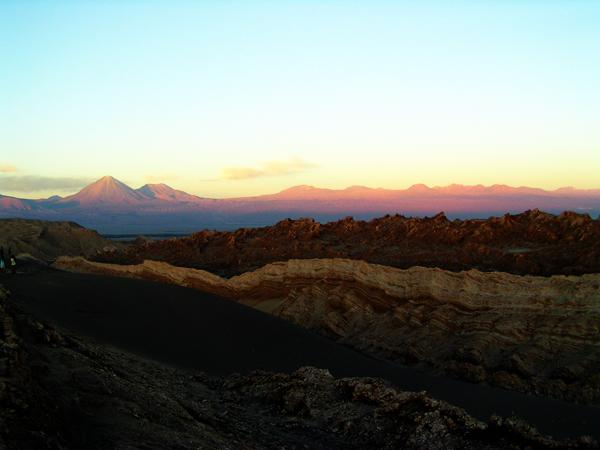
\includegraphics{lum_contfiltre_fvalleluna.jpg}
\caption{`lum\_contfiltre\_fvalleluna.jpg'}
\end{figure}

\begin{itemize}
\tightlist
\item
  Image obtenue avec la fonction de filtre \texttt{g} (accentuation de
  contraste):
\end{itemize}

\begin{figure}
\centering
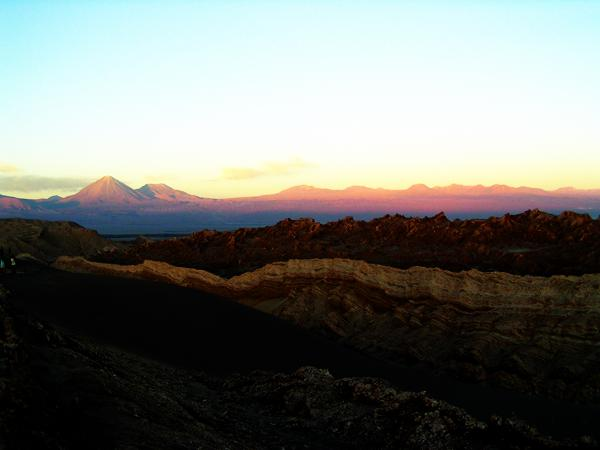
\includegraphics{lum_contfiltre_gvalleluna.jpg}
\caption{`lum\_contfiltre\_gvalleluna.jpg'}
\end{figure}

\begin{itemize}
\tightlist
\item
  Image obtenue avec la fonction de filtre \(x \mapsto x^2\)
  (assombrissement) :
\end{itemize}

\begin{figure}
\centering
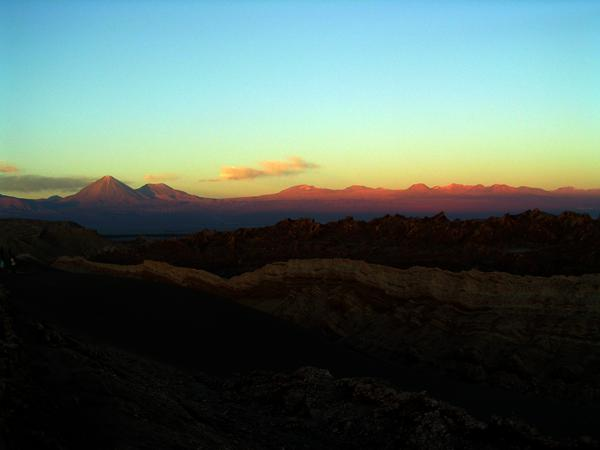
\includegraphics{lum_contfiltre_puissance2valleluna.jpg}
\caption{`lum\_contfiltre\_puissance2valleluna.jpg'}
\end{figure}

\begin{itemize}
\tightlist
\item
  Image obtenue avec la fonction de filtre \(x \mapsto \sqrt{x}\)
  (éclaircissement) :
\end{itemize}

\begin{figure}
\centering
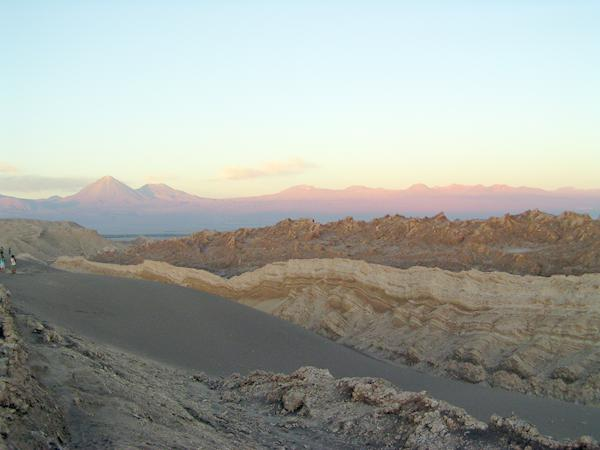
\includegraphics{lum_contfiltre_puissancevalleluna.jpg}
\caption{`lum\_contfiltre\_puissancevalleluna.jpg'}
\end{figure}

    \hypertarget{exercice-7-moyenne-par-blocs}{%
\subsection{\texorpdfstring{Exercice 7 \emph{Moyenne par
blocs}}{Exercice 7 Moyenne par blocs}}\label{exercice-7-moyenne-par-blocs}}

    \begin{Verbatim}[commandchars=\\\{\}]
{\color{incolor}In [{\color{incolor}59}]:} \PY{c+c1}{\PYZsh{} Matrices filtre}
         
         \PY{k}{def} \PY{n+nf}{flou}\PY{p}{(}\PY{n}{k}\PY{p}{)}\PY{p}{:}
             \PY{k}{return} \PY{n}{np}\PY{o}{.}\PY{n}{ones}\PY{p}{(}\PY{p}{(}\PY{l+m+mi}{2}\PY{o}{*}\PY{n}{k}\PY{o}{+}\PY{l+m+mi}{1}\PY{p}{,}\PY{l+m+mi}{2}\PY{o}{*}\PY{n}{k}\PY{o}{+}\PY{l+m+mi}{1}\PY{p}{)}\PY{p}{,}\PY{n}{dtype}\PY{o}{=}\PY{l+s+s2}{\PYZdq{}}\PY{l+s+s2}{uint8}\PY{l+s+s2}{\PYZdq{}}\PY{p}{)}
         
         \PY{n}{flou\PYZus{}bis} \PY{o}{=} \PY{n}{np}\PY{o}{.}\PY{n}{array}\PY{p}{(}\PY{p}{[}\PY{p}{[}\PY{l+m+mi}{1}\PY{p}{,} \PY{l+m+mi}{2}\PY{p}{,} \PY{l+m+mi}{1}\PY{p}{]}\PY{p}{,}
                          \PY{p}{[}\PY{l+m+mi}{2}\PY{p}{,} \PY{l+m+mi}{4}\PY{p}{,} \PY{l+m+mi}{2}\PY{p}{]}\PY{p}{,}
                          \PY{p}{[}\PY{l+m+mi}{1}\PY{p}{,} \PY{l+m+mi}{2}\PY{p}{,} \PY{l+m+mi}{1}\PY{p}{]}\PY{p}{]}\PY{p}{)}
                          
         \PY{n}{A} \PY{o}{=} \PY{n}{np}\PY{o}{.}\PY{n}{array}\PY{p}{(}\PY{p}{[}\PY{p}{[}\PY{o}{\PYZhy{}}\PY{l+m+mi}{1}\PY{p}{,} \PY{o}{\PYZhy{}}\PY{l+m+mi}{2}\PY{p}{,} \PY{o}{\PYZhy{}}\PY{l+m+mi}{1}\PY{p}{]}\PY{p}{,}
                             \PY{p}{[}\PY{o}{\PYZhy{}}\PY{l+m+mi}{2}\PY{p}{,} \PY{l+m+mi}{16}\PY{p}{,} \PY{o}{\PYZhy{}}\PY{l+m+mi}{2}\PY{p}{]}\PY{p}{,}
                             \PY{p}{[}\PY{o}{\PYZhy{}}\PY{l+m+mi}{1}\PY{p}{,} \PY{o}{\PYZhy{}}\PY{l+m+mi}{2}\PY{p}{,} \PY{o}{\PYZhy{}}\PY{l+m+mi}{1}\PY{p}{]}\PY{p}{]}\PY{p}{)}
              
         \PY{n}{B} \PY{o}{=} \PY{n}{np}\PY{o}{.}\PY{n}{array}\PY{p}{(}\PY{p}{[}\PY{p}{[}\PY{l+m+mi}{0}\PY{p}{,} \PY{l+m+mi}{1}\PY{p}{,} \PY{l+m+mi}{0}\PY{p}{]}\PY{p}{,}
              \PY{p}{[}\PY{l+m+mi}{1}\PY{p}{,} \PY{l+m+mi}{1}\PY{p}{,} \PY{l+m+mi}{1}\PY{p}{]}\PY{p}{,}
              \PY{p}{[}\PY{l+m+mi}{0}\PY{p}{,} \PY{l+m+mi}{1}\PY{p}{,} \PY{l+m+mi}{0}\PY{p}{]}\PY{p}{]}\PY{p}{)}
              
         \PY{n}{accentue} \PY{o}{=} \PY{n}{np}\PY{o}{.}\PY{n}{array}\PY{p}{(}\PY{p}{[}\PY{p}{[}\PY{o}{\PYZhy{}}\PY{l+m+mi}{1}\PY{p}{,}\PY{l+m+mi}{1}\PY{p}{,}\PY{o}{\PYZhy{}}\PY{l+m+mi}{1}\PY{p}{,}\PY{l+m+mi}{1}\PY{p}{,}\PY{o}{\PYZhy{}}\PY{l+m+mi}{1}\PY{p}{]}\PY{p}{,}
              \PY{p}{[}\PY{l+m+mi}{1}\PY{p}{,}\PY{o}{\PYZhy{}}\PY{l+m+mi}{1}\PY{p}{,} \PY{o}{\PYZhy{}}\PY{l+m+mi}{2}\PY{p}{,} \PY{o}{\PYZhy{}}\PY{l+m+mi}{1}\PY{p}{,}\PY{l+m+mi}{1}\PY{p}{]}\PY{p}{,}
              \PY{p}{[}\PY{o}{\PYZhy{}}\PY{l+m+mi}{1}\PY{p}{,}\PY{o}{\PYZhy{}}\PY{l+m+mi}{2}\PY{p}{,} \PY{l+m+mi}{16}\PY{p}{,} \PY{o}{\PYZhy{}}\PY{l+m+mi}{2}\PY{p}{,}\PY{o}{\PYZhy{}}\PY{l+m+mi}{1}\PY{p}{]}\PY{p}{,}
              \PY{p}{[}\PY{l+m+mi}{1}\PY{p}{,}\PY{o}{\PYZhy{}}\PY{l+m+mi}{1}\PY{p}{,} \PY{o}{\PYZhy{}}\PY{l+m+mi}{2}\PY{p}{,} \PY{o}{\PYZhy{}}\PY{l+m+mi}{1}\PY{p}{,}\PY{l+m+mi}{1}\PY{p}{]}\PY{p}{,}
              \PY{p}{[}\PY{o}{\PYZhy{}}\PY{l+m+mi}{1}\PY{p}{,}\PY{l+m+mi}{1}\PY{p}{,}\PY{o}{\PYZhy{}}\PY{l+m+mi}{1}\PY{p}{,}\PY{l+m+mi}{1}\PY{p}{,}\PY{o}{\PYZhy{}}\PY{l+m+mi}{1}\PY{p}{]}\PY{p}{]}\PY{p}{)}
         
         \PY{c+c1}{\PYZsh{} Filtre de repoussage (emboss)}
         \PY{n}{C} \PY{o}{=} \PY{n}{np}\PY{o}{.}\PY{n}{array}\PY{p}{(}\PY{p}{[}\PY{p}{[}\PY{l+m+mi}{2}\PY{p}{,} \PY{l+m+mi}{1}\PY{p}{,} \PY{l+m+mi}{0}\PY{p}{]}\PY{p}{,}
              \PY{p}{[}\PY{l+m+mi}{1}\PY{p}{,} \PY{l+m+mi}{1}\PY{p}{,} \PY{o}{\PYZhy{}}\PY{l+m+mi}{1}\PY{p}{]}\PY{p}{,}
              \PY{p}{[}\PY{l+m+mi}{0}\PY{p}{,} \PY{o}{\PYZhy{}}\PY{l+m+mi}{1}\PY{p}{,} \PY{o}{\PYZhy{}}\PY{l+m+mi}{2}\PY{p}{]}\PY{p}{]}\PY{p}{)}
              
         \PY{n}{D} \PY{o}{=} \PY{n}{np}\PY{o}{.}\PY{n}{array}\PY{p}{(}\PY{p}{[}\PY{p}{[}\PY{o}{\PYZhy{}}\PY{l+m+mi}{2}\PY{p}{,} \PY{o}{\PYZhy{}}\PY{l+m+mi}{1}\PY{p}{,} \PY{l+m+mi}{0}\PY{p}{]}\PY{p}{,}
              \PY{p}{[}\PY{o}{\PYZhy{}}\PY{l+m+mi}{1}\PY{p}{,} \PY{l+m+mi}{1}\PY{p}{,} \PY{l+m+mi}{1}\PY{p}{]}\PY{p}{,}
              \PY{p}{[}\PY{l+m+mi}{0}\PY{p}{,} \PY{l+m+mi}{1}\PY{p}{,} \PY{l+m+mi}{2}\PY{p}{]}\PY{p}{]}\PY{p}{)}
         
         \PY{c+c1}{\PYZsh{} Détection de bords}
         \PY{n}{E} \PY{o}{=} \PY{n}{np}\PY{o}{.}\PY{n}{array}\PY{p}{(}\PY{p}{[}\PY{p}{[}\PY{o}{\PYZhy{}}\PY{l+m+mi}{1}\PY{o}{/}\PY{l+m+mi}{9}\PY{p}{,} \PY{o}{\PYZhy{}}\PY{l+m+mi}{1}\PY{o}{/}\PY{l+m+mi}{9}\PY{p}{,} \PY{o}{\PYZhy{}}\PY{l+m+mi}{1}\PY{o}{/}\PY{l+m+mi}{9}\PY{p}{]}\PY{p}{,}
              \PY{p}{[}\PY{o}{\PYZhy{}}\PY{l+m+mi}{1}\PY{o}{/}\PY{l+m+mi}{9}\PY{p}{,} \PY{l+m+mi}{8}\PY{o}{/}\PY{l+m+mi}{9}\PY{p}{,} \PY{o}{\PYZhy{}}\PY{l+m+mi}{1}\PY{o}{/}\PY{l+m+mi}{9}\PY{p}{]}\PY{p}{,}
              \PY{p}{[}\PY{o}{\PYZhy{}}\PY{l+m+mi}{1}\PY{o}{/}\PY{l+m+mi}{9}\PY{p}{,} \PY{o}{\PYZhy{}}\PY{l+m+mi}{1}\PY{o}{/}\PY{l+m+mi}{9}\PY{p}{,} \PY{o}{\PYZhy{}}\PY{l+m+mi}{1}\PY{o}{/}\PY{l+m+mi}{9}\PY{p}{]}\PY{p}{]}\PY{p}{)}
              
         \PY{n}{F} \PY{o}{=} \PY{n}{np}\PY{o}{.}\PY{n}{array}\PY{p}{(}\PY{p}{[}\PY{p}{[}\PY{l+m+mi}{0}\PY{p}{,} \PY{o}{\PYZhy{}}\PY{l+m+mi}{1}\PY{p}{,} \PY{l+m+mi}{0}\PY{p}{]}\PY{p}{,}
              \PY{p}{[}\PY{o}{\PYZhy{}}\PY{l+m+mi}{1}\PY{p}{,} \PY{l+m+mi}{4}\PY{p}{,} \PY{o}{\PYZhy{}}\PY{l+m+mi}{1}\PY{p}{]}\PY{p}{,}
              \PY{p}{[}\PY{l+m+mi}{0}\PY{p}{,} \PY{o}{\PYZhy{}}\PY{l+m+mi}{1}\PY{p}{,} \PY{l+m+mi}{0}\PY{p}{]}\PY{p}{]}\PY{p}{)}
             
         \PY{n}{G} \PY{o}{=} \PY{n}{np}\PY{o}{.}\PY{n}{array}\PY{p}{(}\PY{p}{[}\PY{p}{[}\PY{l+m+mi}{1}\PY{p}{,} \PY{l+m+mi}{0}\PY{p}{,} \PY{o}{\PYZhy{}}\PY{l+m+mi}{1}\PY{p}{]}\PY{p}{,}
              \PY{p}{[}\PY{l+m+mi}{1}\PY{p}{,} \PY{l+m+mi}{0}\PY{p}{,} \PY{o}{\PYZhy{}}\PY{l+m+mi}{1}\PY{p}{]}\PY{p}{,}
              \PY{p}{[}\PY{l+m+mi}{1}\PY{p}{,} \PY{l+m+mi}{0}\PY{p}{,} \PY{o}{\PYZhy{}}\PY{l+m+mi}{1}\PY{p}{]}\PY{p}{]}\PY{p}{)}
              
         \PY{n}{H} \PY{o}{=} \PY{n}{np}\PY{o}{.}\PY{n}{array}\PY{p}{(}\PY{p}{[}\PY{p}{[}\PY{o}{\PYZhy{}}\PY{l+m+mi}{1}\PY{p}{,} \PY{o}{\PYZhy{}}\PY{l+m+mi}{2}\PY{p}{,} \PY{o}{\PYZhy{}}\PY{l+m+mi}{1}\PY{p}{]}\PY{p}{,}
              \PY{p}{[}\PY{l+m+mi}{0}\PY{p}{,} \PY{l+m+mi}{0}\PY{p}{,} \PY{l+m+mi}{0}\PY{p}{]}\PY{p}{,}
              \PY{p}{[}\PY{l+m+mi}{1}\PY{p}{,} \PY{l+m+mi}{2}\PY{p}{,} \PY{l+m+mi}{1}\PY{p}{]}\PY{p}{]}\PY{p}{)}
\end{Verbatim}


    \begin{Verbatim}[commandchars=\\\{\}]
{\color{incolor}In [{\color{incolor}54}]:} \PY{k}{def}  \PY{n+nf}{moyenne\PYZus{}bloc}\PY{p}{(}\PY{n}{pixels}\PY{p}{,} \PY{n}{i}\PY{p}{,} \PY{n}{j}\PY{p}{,} \PY{n}{matrice}\PY{p}{)}\PY{p}{:}
             \PY{l+s+sd}{\PYZdq{}\PYZdq{}\PYZdq{}Fait la convolution de la matrice pixels par la matrice passée en paramètre\PYZdq{}\PYZdq{}\PYZdq{}}
             \PY{n}{rayonbloc} \PY{o}{=} \PY{n+nb}{len}\PY{p}{(}\PY{n}{matrice}\PY{p}{)} \PY{o}{/}\PY{o}{/} \PY{l+m+mi}{2}  \PY{c+c1}{\PYZsh{}matrice carrée avec des dimensions impaires}
             \PY{n}{somme\PYZus{}coef} \PY{o}{=} \PY{n}{np}\PY{o}{.}\PY{n}{sum}\PY{p}{(}\PY{n}{matrice}\PY{p}{)}
             \PY{k}{if} \PY{n}{somme\PYZus{}coef} \PY{o}{==} \PY{l+m+mi}{0}\PY{p}{:}
                 \PY{n}{somme\PYZus{}coef} \PY{o}{=} \PY{l+m+mi}{1}
             \PY{n}{hauteur}\PY{p}{,} \PY{n}{largeur} \PY{o}{=} \PY{n}{pixels}\PY{o}{.}\PY{n}{shape}\PY{p}{[}\PY{p}{:}\PY{l+m+mi}{2}\PY{p}{]}
             \PY{c+c1}{\PYZsh{}si pixels est une matrice de pixels en niveau de gris}
             \PY{k}{if} \PY{n+nb}{len}\PY{p}{(}\PY{n}{pixels}\PY{o}{.}\PY{n}{shape}\PY{p}{)} \PY{o}{==} \PY{l+m+mi}{2}\PY{p}{:}
                 \PY{k}{return} \PY{n}{maxmin}\PY{p}{(}\PY{n}{np}\PY{o}{.}\PY{n}{sum}\PY{p}{(}\PY{n}{pixels}\PY{p}{[}\PY{n}{i} \PY{o}{\PYZhy{}} \PY{n}{rayonbloc} \PY{p}{:} \PY{n}{i} \PY{o}{+} \PY{n}{rayonbloc} \PY{o}{+} \PY{l+m+mi}{1}\PY{p}{,} \PY{n}{j} \PY{o}{\PYZhy{}} \PY{n}{rayonbloc} \PY{p}{:} \PY{n}{j} \PY{o}{+} \PY{n}{rayonbloc} \PY{o}{+} \PY{l+m+mi}{1}\PY{p}{]} \PY{o}{*} \PY{n}{matrice}\PY{p}{)} \PY{o}{/} \PY{n}{somme\PYZus{}coef}\PY{p}{)}
             \PY{k}{else}\PY{p}{:} \PY{c+c1}{\PYZsh{}si pixels est une matrice de pixels couleurs en (R,G,B)}
                 \PY{k}{return} \PY{p}{[}\PY{n}{maxmin}\PY{p}{(}\PY{n}{np}\PY{o}{.}\PY{n}{sum}\PY{p}{(}\PY{n}{pixels}\PY{p}{[}\PY{n}{i} \PY{o}{\PYZhy{}} \PY{n}{rayonbloc} \PY{p}{:} \PY{n}{i} \PY{o}{+} \PY{n}{rayonbloc} \PY{o}{+} \PY{l+m+mi}{1}\PY{p}{,} \PY{n}{j} \PY{o}{\PYZhy{}} \PY{n}{rayonbloc} \PY{p}{:} \PY{n}{j} \PY{o}{+} \PY{n}{rayonbloc} \PY{o}{+} \PY{l+m+mi}{1}\PY{p}{,} \PY{n}{k}\PY{p}{]} \PY{o}{*} \PY{n}{matrice}\PY{p}{)} \PY{o}{/} \PY{n}{somme\PYZus{}coef}\PY{p}{)} \PYZbs{}
                         \PY{k}{for} \PY{n}{k} \PY{o+ow}{in} \PY{n+nb}{range}\PY{p}{(}\PY{l+m+mi}{3}\PY{p}{)}\PY{p}{]}
             \PY{k}{return} \PY{n}{pixels\PYZus{}res}    
         
         
         \PY{k}{def} \PY{n+nf}{moyenne\PYZus{}bloc2}\PY{p}{(}\PY{n}{pixels}\PY{p}{,} \PY{n}{i}\PY{p}{,} \PY{n}{j}\PY{p}{,} \PY{n}{matrice}\PY{p}{)}\PY{p}{:}
             \PY{n}{rayonbloc} \PY{o}{=} \PY{n+nb}{len}\PY{p}{(}\PY{n}{matrice}\PY{p}{)}\PY{o}{/}\PY{o}{/}\PY{l+m+mi}{2}
             \PY{k}{if} \PY{n}{np}\PY{o}{.}\PY{n}{sum}\PY{p}{(}\PY{n}{matrice}\PY{p}{)}\PY{o}{==}\PY{l+m+mi}{0}\PY{p}{:}
                 \PY{n}{som\PYZus{}matrice}\PY{o}{=}\PY{l+m+mi}{1}
             \PY{k}{else}\PY{p}{:}
                 \PY{n}{som\PYZus{}matrice}\PY{o}{=}\PY{n}{np}\PY{o}{.}\PY{n}{sum}\PY{p}{(}\PY{n}{matrice}\PY{p}{)}
             \PY{k}{if} \PY{n+nb}{len}\PY{p}{(}\PY{n}{pixels}\PY{o}{.}\PY{n}{shape}\PY{p}{)}\PY{o}{==}\PY{l+m+mi}{3}\PY{p}{:}
                 \PY{n}{pixel}\PY{o}{=}\PY{p}{[}\PY{l+m+mi}{0}\PY{p}{,}\PY{l+m+mi}{0}\PY{p}{,}\PY{l+m+mi}{0}\PY{p}{]}
                 \PY{k}{for} \PY{n}{k} \PY{o+ow}{in} \PY{n+nb}{range}\PY{p}{(}\PY{l+m+mi}{3}\PY{p}{)}\PY{p}{:}
                     \PY{n}{pixel}\PY{p}{[}\PY{n}{k}\PY{p}{]}\PY{o}{=}\PY{n}{maxmin}\PY{p}{(}\PY{n}{np}\PY{o}{.}\PY{n}{sum}\PY{p}{(}\PY{n}{pixels}\PY{p}{[}\PY{n}{i}\PY{o}{\PYZhy{}}\PY{n}{rayonbloc}\PY{p}{:}\PY{n}{i}\PY{o}{+}\PY{n}{rayonbloc}\PY{o}{+}\PY{l+m+mi}{1}\PY{p}{,} \PY{n}{j}\PY{o}{\PYZhy{}}\PY{n}{rayonbloc}\PY{p}{:}\PY{n}{j}\PY{o}{+}\PY{n}{rayonbloc}\PY{o}{+}\PY{l+m+mi}{1}\PY{p}{,}\PY{n}{k}\PY{p}{]}\PY{o}{*}\PY{n}{matrice}\PY{p}{)}\PY{o}{/}\PY{o}{/}\PY{n}{som\PYZus{}matrice}\PY{p}{)}
             \PY{k}{else} \PY{p}{:}
                 \PY{n}{pixel}\PY{o}{=}\PY{n}{maxmin}\PY{p}{(}\PY{n}{np}\PY{o}{.}\PY{n}{sum}\PY{p}{(}\PY{n}{pixels}\PY{p}{[}\PY{n}{i}\PY{o}{\PYZhy{}}\PY{n}{rayonbloc}\PY{p}{:}\PY{n}{i}\PY{o}{+}\PY{n}{rayonbloc}\PY{o}{+}\PY{l+m+mi}{1}\PY{p}{,} \PY{n}{j}\PY{o}{\PYZhy{}}\PY{n}{rayonbloc}\PY{p}{:}\PY{n}{j}\PY{o}{+}\PY{n}{rayonbloc}\PY{o}{+}\PY{l+m+mi}{1}\PY{p}{]}\PY{o}{*}\PY{n}{matrice}\PY{p}{)}\PY{o}{/}\PY{o}{/}\PY{n}{som\PYZus{}matrice}\PY{p}{)}
             \PY{k}{return} \PY{n}{pixel}
             
         
         \PY{k}{def} \PY{n+nf}{applique\PYZus{}filtre}\PY{p}{(}\PY{n}{imsource}\PY{p}{,} \PY{n}{matrice}\PY{p}{,} \PY{n}{filtre} \PY{o}{=}\PY{l+s+s2}{\PYZdq{}}\PY{l+s+s2}{filtre}\PY{l+s+s2}{\PYZdq{}}\PY{p}{)}\PY{p}{:}
             \PY{n}{im} \PY{o}{=} \PY{n}{Image}\PY{o}{.}\PY{n}{open}\PY{p}{(}\PY{n}{imsource}\PY{p}{)}
             \PY{n}{pixels} \PY{o}{=} \PY{n}{np}\PY{o}{.}\PY{n}{array}\PY{p}{(}\PY{n}{im}\PY{p}{)}
             \PY{n}{hauteur}\PY{p}{,} \PY{n}{largeur} \PY{o}{=} \PY{n}{pixels}\PY{o}{.}\PY{n}{shape}\PY{p}{[}\PY{p}{:}\PY{l+m+mi}{2}\PY{p}{]}
             \PY{n}{pixels\PYZus{}res} \PY{o}{=} \PY{n}{np}\PY{o}{.}\PY{n}{zeros\PYZus{}like}\PY{p}{(}\PY{n}{pixels}\PY{p}{)}
             \PY{n}{rayonbloc} \PY{o}{=} \PY{n+nb}{len}\PY{p}{(}\PY{n}{matrice}\PY{p}{)}\PY{o}{/}\PY{o}{/}\PY{l+m+mi}{2}
             \PY{k}{for} \PY{n}{i} \PY{o+ow}{in} \PY{n+nb}{range}\PY{p}{(}\PY{n}{rayonbloc}\PY{p}{,}\PY{n}{hauteur}\PY{o}{\PYZhy{}}\PY{n}{rayonbloc}\PY{p}{)}\PY{p}{:}
                 \PY{k}{for} \PY{n}{j} \PY{o+ow}{in} \PY{n+nb}{range}\PY{p}{(}\PY{n}{rayonbloc}\PY{p}{,}\PY{n}{largeur}\PY{o}{\PYZhy{}}\PY{n}{rayonbloc}\PY{p}{)}\PY{p}{:}
                     \PY{n}{pixels\PYZus{}res}\PY{p}{[}\PY{n}{i}\PY{p}{,}\PY{n}{j}\PY{p}{]} \PY{o}{=} \PY{n}{moyenne\PYZus{}bloc}\PY{p}{(}\PY{n}{pixels}\PY{p}{,}\PY{n}{i}\PY{p}{,}\PY{n}{j}\PY{p}{,}\PY{n}{matrice}\PY{p}{)}
             \PY{n}{img\PYZus{}res} \PY{o}{=} \PY{n}{Image}\PY{o}{.}\PY{n}{fromarray}\PY{p}{(}\PY{n}{pixels\PYZus{}res}\PY{p}{)}
             \PY{n}{img\PYZus{}res}\PY{o}{.}\PY{n}{save}\PY{p}{(}\PY{n}{filtre} \PY{o}{+} \PY{n}{imsource}\PY{p}{)}
             \PY{n}{img\PYZus{}res}\PY{o}{.}\PY{n}{show}\PY{p}{(}\PY{p}{)}   
\end{Verbatim}


    \begin{Verbatim}[commandchars=\\\{\}]
{\color{incolor}In [{\color{incolor}55}]:} \PY{n}{flou\PYZus{}bis} \PY{o}{=} \PY{n}{np}\PY{o}{.}\PY{n}{array}\PY{p}{(}\PY{p}{[}\PY{p}{[}\PY{l+m+mi}{1}\PY{p}{,} \PY{l+m+mi}{2}\PY{p}{,} \PY{l+m+mi}{1}\PY{p}{]}\PY{p}{,}
                          \PY{p}{[}\PY{l+m+mi}{2}\PY{p}{,} \PY{l+m+mi}{4}\PY{p}{,} \PY{l+m+mi}{2}\PY{p}{]}\PY{p}{,}
                          \PY{p}{[}\PY{l+m+mi}{1}\PY{p}{,} \PY{l+m+mi}{2}\PY{p}{,} \PY{l+m+mi}{1}\PY{p}{]}\PY{p}{]}\PY{p}{)}
\end{Verbatim}


    \begin{Verbatim}[commandchars=\\\{\}]
{\color{incolor}In [{\color{incolor}56}]:} \PY{n}{applique\PYZus{}filtre}\PY{p}{(}\PY{l+s+s1}{\PYZsq{}}\PY{l+s+s1}{valleluna.jpg}\PY{l+s+s1}{\PYZsq{}}\PY{p}{,} \PY{n}{flou\PYZus{}bis}\PY{p}{,} \PY{n}{filtre} \PY{o}{=} \PY{l+s+s2}{\PYZdq{}}\PY{l+s+s2}{flou\PYZus{}}\PY{l+s+s2}{\PYZdq{}}\PY{p}{)}
\end{Verbatim}


    \begin{Verbatim}[commandchars=\\\{\}]
{\color{incolor}In [{\color{incolor}60}]:} \PY{n}{A}
\end{Verbatim}


\begin{Verbatim}[commandchars=\\\{\}]
{\color{outcolor}Out[{\color{outcolor}60}]:} array([[-1, -2, -1],
                [-2, 16, -2],
                [-1, -2, -1]])
\end{Verbatim}
            
    \begin{Verbatim}[commandchars=\\\{\}]
{\color{incolor}In [{\color{incolor}61}]:} \PY{n}{applique\PYZus{}filtre}\PY{p}{(}\PY{l+s+s1}{\PYZsq{}}\PY{l+s+s1}{valleluna.jpg}\PY{l+s+s1}{\PYZsq{}}\PY{p}{,} \PY{n}{A}\PY{p}{,} \PY{n}{filtre} \PY{o}{=} \PY{l+s+s2}{\PYZdq{}}\PY{l+s+s2}{filtre\PYZus{}net\PYZus{}}\PY{l+s+s2}{\PYZdq{}}\PY{p}{)}
\end{Verbatim}


    \begin{itemize}
\tightlist
\item
  Application du filtre de floutage gaussien
  \(M = \begin{pmatrix} 1 & 2 & 1 \\ 2 & 4 & 2 \\ 1 & 2 & 1 \end{pmatrix}\)
\end{itemize}

\begin{figure}
\centering
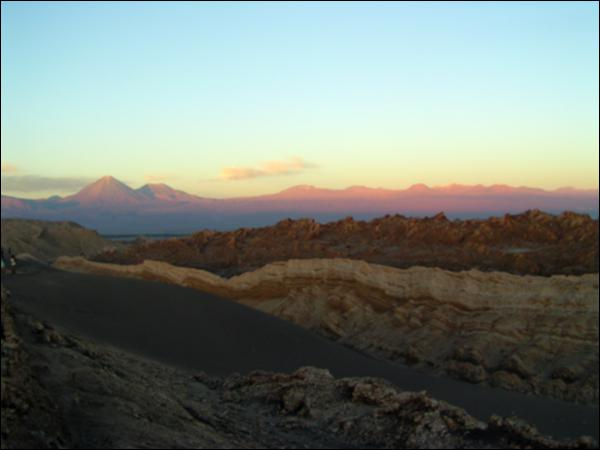
\includegraphics{flou_valleluna.jpg}
\caption{`floutage\_valleluna.jpg'}
\end{figure}

\begin{itemize}
\tightlist
\item
  Application du filtre de convolution de la matrice
  \(A=\begin{pmatrix} 0&0&0\\0&20&0\\0&0&0 \end{pmatrix}-M=\begin{pmatrix} -1&-2&-1\\-2&16&-2\\-1&-2&-1 \end{pmatrix}\)
  (Augmentation du contraste)
\end{itemize}

\begin{figure}
\centering
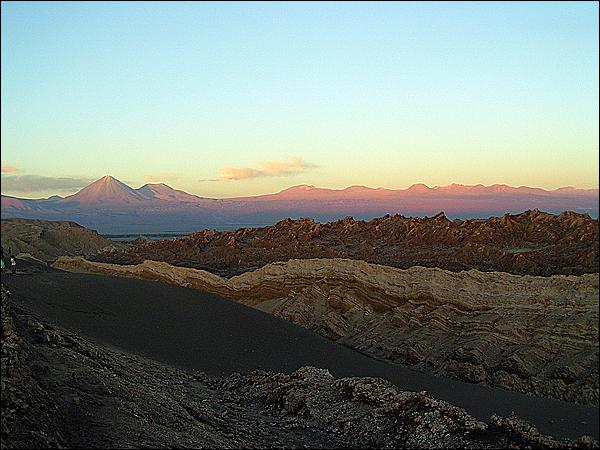
\includegraphics{filtre_net_valleluna.jpg}
\caption{`filtrevalleluna.jpg'}
\end{figure}

    \hypertarget{exercice-8-pixellisation}{%
\subsection{\texorpdfstring{Exercice 8
\emph{Pixellisation}}{Exercice 8 Pixellisation}}\label{exercice-8-pixellisation}}

    \begin{Verbatim}[commandchars=\\\{\}]
{\color{incolor}In [{\color{incolor}26}]:} \PY{k}{def}  \PY{n+nf}{pixellisation}\PY{p}{(}\PY{n}{imsource}\PY{p}{,} \PY{n}{taillebloc}\PY{p}{)}\PY{p}{:}
             \PY{n}{im} \PY{o}{=} \PY{n}{Image}\PY{o}{.}\PY{n}{open}\PY{p}{(}\PY{n}{imsource}\PY{p}{)}
             \PY{n}{pixels} \PY{o}{=} \PY{n}{np}\PY{o}{.}\PY{n}{array}\PY{p}{(}\PY{n}{im}\PY{p}{)}
             \PY{n}{hauteur}\PY{p}{,} \PY{n}{largeur} \PY{o}{=} \PY{n}{pixels}\PY{o}{.}\PY{n}{shape}\PY{p}{[}\PY{p}{:}\PY{l+m+mi}{2}\PY{p}{]}
             \PY{n}{pixels\PYZus{}res} \PY{o}{=} \PY{n}{np}\PY{o}{.}\PY{n}{zeros\PYZus{}like}\PY{p}{(}\PY{n}{pixels}\PY{p}{)}
             \PY{k}{for} \PY{n}{i} \PY{o+ow}{in} \PY{n+nb}{range}\PY{p}{(}\PY{l+m+mi}{0}\PY{p}{,} \PY{n}{hauteur} \PY{o}{\PYZhy{}} \PY{n}{taillebloc} \PY{o}{+} \PY{l+m+mi}{1}\PY{p}{,} \PY{n}{taillebloc}\PY{p}{)}\PY{p}{:}
                 \PY{k}{for} \PY{n}{j} \PY{o+ow}{in} \PY{n+nb}{range}\PY{p}{(}\PY{l+m+mi}{0}\PY{p}{,} \PY{n}{largeur} \PY{o}{\PYZhy{}} \PY{n}{taillebloc} \PY{o}{+} \PY{l+m+mi}{1}\PY{p}{,} \PY{n}{taillebloc}\PY{p}{)}\PY{p}{:}
                     \PY{n}{pixel\PYZus{}moyen} \PY{o}{=} \PY{p}{[}\PY{l+m+mi}{0}\PY{p}{,} \PY{l+m+mi}{0}\PY{p}{,} \PY{l+m+mi}{0}\PY{p}{]}
                     \PY{k}{for} \PY{n}{k} \PY{o+ow}{in} \PY{n+nb}{range}\PY{p}{(}\PY{l+m+mi}{3}\PY{p}{)}\PY{p}{:}
                         \PY{n}{pixel\PYZus{}moyen}\PY{p}{[}\PY{n}{k}\PY{p}{]} \PY{o}{=} \PY{n+nb}{int}\PY{p}{(}\PY{n}{np}\PY{o}{.}\PY{n}{mean}\PY{p}{(}\PY{n}{pixels}\PY{p}{[}\PY{n}{i} \PY{p}{:} \PY{n}{i} \PY{o}{+} \PY{n}{taillebloc}\PY{p}{,} \PY{n}{j} \PY{p}{:} \PY{n}{j} \PY{o}{+} \PY{n}{taillebloc}\PY{p}{,}\PY{n}{k}\PY{p}{]}\PY{p}{)}\PY{p}{)}
                     \PY{c+c1}{\PYZsh{}pixels\PYZus{}res[i : i + taille\PYZus{}bloc, j : j + taille\PYZus{}bloc] =  np.array([[pixel\PYZus{}moyen for \PYZus{} in range(taille\PYZus{}bloc)]for \PYZus{} in range(taille\PYZus{}bloc)])}
                     \PY{k}{for} \PY{n}{x} \PY{o+ow}{in} \PY{n+nb}{range}\PY{p}{(}\PY{n}{taillebloc}\PY{p}{)}\PY{p}{:}
                         \PY{k}{for} \PY{n}{y} \PY{o+ow}{in} \PY{n+nb}{range}\PY{p}{(}\PY{n}{taillebloc}\PY{p}{)}\PY{p}{:}
                             \PY{n}{pixels\PYZus{}res}\PY{p}{[}\PY{n}{i} \PY{o}{+} \PY{n}{x}\PY{p}{,} \PY{n}{j} \PY{o}{+} \PY{n}{y}\PY{p}{]} \PY{o}{=} \PY{n}{pixel\PYZus{}moyen}
             \PY{n}{img\PYZus{}res} \PY{o}{=} \PY{n}{Image}\PY{o}{.}\PY{n}{fromarray}\PY{p}{(}\PY{n}{pixels\PYZus{}res}\PY{p}{)}
             \PY{n}{img\PYZus{}res}\PY{o}{.}\PY{n}{save}\PY{p}{(}\PY{l+s+s2}{\PYZdq{}}\PY{l+s+s2}{pixel\PYZus{}}\PY{l+s+s2}{\PYZdq{}}\PY{o}{+}\PY{n}{imsource}\PY{p}{)}
             \PY{n}{img\PYZus{}res}\PY{o}{.}\PY{n}{show}\PY{p}{(}\PY{p}{)}   
             
             
         \PY{k}{def} \PY{n+nf}{pixellisation2}\PY{p}{(}\PY{n}{imsource}\PY{p}{,}\PY{n}{taillebloc}\PY{p}{)}\PY{p}{:}
             \PY{n}{im}\PY{o}{=}\PY{n}{Image}\PY{o}{.}\PY{n}{open}\PY{p}{(}\PY{n}{imsource}\PY{p}{)}
             \PY{n}{pixels} \PY{o}{=} \PY{n}{np}\PY{o}{.}\PY{n}{array}\PY{p}{(}\PY{n}{im}\PY{p}{)}
             \PY{n}{hauteur}\PY{p}{,} \PY{n}{largeur} \PY{o}{=}\PY{n}{pixels}\PY{o}{.}\PY{n}{shape}\PY{p}{[}\PY{p}{:}\PY{l+m+mi}{2}\PY{p}{]}
             \PY{n}{pixels} \PY{o}{=} \PY{n}{pixels}\PY{o}{.}\PY{n}{astype}\PY{p}{(}\PY{n+nb}{int}\PY{p}{)}
             \PY{n}{pixels\PYZus{}res} \PY{o}{=} \PY{n}{np}\PY{o}{.}\PY{n}{zeros\PYZus{}like}\PY{p}{(}\PY{n}{pixels}\PY{p}{)}
             \PY{k}{for} \PY{n}{i} \PY{o+ow}{in} \PY{n+nb}{range}\PY{p}{(}\PY{l+m+mi}{0}\PY{p}{,}\PY{n}{hauteur}\PY{o}{\PYZhy{}}\PY{n}{taillebloc}\PY{o}{+}\PY{l+m+mi}{1}\PY{p}{,}\PY{n}{taillebloc}\PY{p}{)}\PY{p}{:}
                 \PY{k}{for} \PY{n}{j} \PY{o+ow}{in} \PY{n+nb}{range}\PY{p}{(}\PY{l+m+mi}{0}\PY{p}{,}\PY{n}{largeur}\PY{o}{\PYZhy{}}\PY{n}{taillebloc}\PY{o}{+}\PY{l+m+mi}{1}\PY{p}{,}\PY{n}{taillebloc}\PY{p}{)}\PY{p}{:}
                     \PY{k}{for} \PY{n}{k} \PY{o+ow}{in} \PY{n+nb}{range}\PY{p}{(}\PY{l+m+mi}{3}\PY{p}{)}\PY{p}{:}
                         \PY{n}{couleur} \PY{o}{=} \PY{n}{np}\PY{o}{.}\PY{n}{mean}\PY{p}{(}\PY{n}{pixels}\PY{p}{[}\PY{n}{i}\PY{p}{:}\PY{n}{i}\PY{o}{+}\PY{n}{taillebloc}\PY{p}{,}\PY{n}{j}\PY{p}{:}\PY{n}{j}\PY{o}{+}\PY{n}{taillebloc}\PY{p}{,}\PY{n}{k}\PY{p}{]}\PY{p}{)}
                         \PY{k}{for} \PY{n}{x} \PY{o+ow}{in} \PY{n+nb}{range}\PY{p}{(}\PY{n}{taillebloc}\PY{p}{)}\PY{p}{:}
                             \PY{k}{for} \PY{n}{y} \PY{o+ow}{in} \PY{n+nb}{range}\PY{p}{(}\PY{n}{taillebloc}\PY{p}{)}\PY{p}{:}
                                 \PY{n}{pixels\PYZus{}res}\PY{p}{[}\PY{n}{i}\PY{o}{+}\PY{n}{x}\PY{p}{,}\PY{n}{j}\PY{o}{+}\PY{n}{y}\PY{p}{,}\PY{n}{k}\PY{p}{]} \PY{o}{=} \PY{n}{couleur}
             \PY{n}{pixels\PYZus{}res}\PY{o}{=}\PY{n}{pixels\PYZus{}res}\PY{o}{.}\PY{n}{astype}\PY{p}{(}\PY{n}{np}\PY{o}{.}\PY{n}{uint8}\PY{p}{)}
             \PY{n}{img\PYZus{}res} \PY{o}{=} \PY{n}{Image}\PY{o}{.}\PY{n}{fromarray}\PY{p}{(}\PY{n}{pixels\PYZus{}res}\PY{p}{)}
             \PY{n}{img\PYZus{}res}\PY{o}{.}\PY{n}{save}\PY{p}{(}\PY{l+s+s2}{\PYZdq{}}\PY{l+s+s2}{pixel\PYZus{}}\PY{l+s+s2}{\PYZdq{}} \PY{o}{+} \PY{n+nb}{str}\PY{p}{(}\PY{n}{taillebloc}\PY{p}{)} \PY{o}{+} \PY{l+s+s2}{\PYZdq{}}\PY{l+s+s2}{\PYZus{}}\PY{l+s+s2}{\PYZdq{}} \PY{o}{+} \PY{n}{imsource}\PY{p}{)}
             \PY{n}{img\PYZus{}res}\PY{o}{.}\PY{n}{show}\PY{p}{(}\PY{p}{)}
\end{Verbatim}


    \begin{Verbatim}[commandchars=\\\{\}]
{\color{incolor}In [{\color{incolor}44}]:} \PY{n}{pixellisation}\PY{p}{(}\PY{l+s+s1}{\PYZsq{}}\PY{l+s+s1}{valleluna.jpg}\PY{l+s+s1}{\PYZsq{}}\PY{p}{,} \PY{l+m+mi}{10}\PY{p}{)}
\end{Verbatim}


    \begin{Verbatim}[commandchars=\\\{\}]
{\color{incolor}In [{\color{incolor}24}]:} \PY{n}{pixellisation2}\PY{p}{(}\PY{l+s+s1}{\PYZsq{}}\PY{l+s+s1}{valleluna.jpg}\PY{l+s+s1}{\PYZsq{}}\PY{p}{,} \PY{l+m+mi}{10}\PY{p}{)}
\end{Verbatim}


    \begin{itemize}
\tightlist
\item
  Image pixellisée avec des blocs de \(10\) pixels de côté :
\end{itemize}

\begin{figure}
\centering
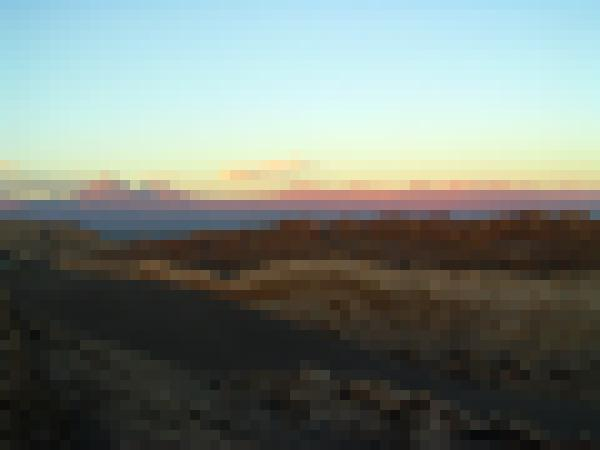
\includegraphics{pixel_valleluna.jpg}
\caption{`pixel\_valleluna.jpg'}
\end{figure}

    \hypertarget{exercice-9-seuillage}{%
\subsection{Exercice 9 : seuillage}\label{exercice-9-seuillage}}

    \begin{Verbatim}[commandchars=\\\{\}]
{\color{incolor}In [{\color{incolor}91}]:} \PY{k}{def} \PY{n+nf}{seuillage}\PY{p}{(}\PY{n}{imsource}\PY{p}{,} \PY{n}{s}\PY{p}{)}\PY{p}{:}
             \PY{n}{im} \PY{o}{=} \PY{n}{Image}\PY{o}{.}\PY{n}{open}\PY{p}{(}\PY{n}{imsource}\PY{p}{)}
             \PY{n}{pixels} \PY{o}{=} \PY{n}{np}\PY{o}{.}\PY{n}{array}\PY{p}{(}\PY{n}{im}\PY{p}{)}
             \PY{k}{assert} \PY{n+nb}{len}\PY{p}{(}\PY{n}{pixels}\PY{o}{.}\PY{n}{shape}\PY{p}{)} \PY{o}{==} \PY{l+m+mi}{2}\PY{p}{,} \PY{l+s+s2}{\PYZdq{}}\PY{l+s+s2}{l}\PY{l+s+s2}{\PYZsq{}}\PY{l+s+s2}{image doit être en niveau de gris}\PY{l+s+s2}{\PYZdq{}}
             \PY{n}{hauteur}\PY{p}{,} \PY{n}{largeur} \PY{o}{=} \PY{n}{pixels}\PY{o}{.}\PY{n}{shape}\PY{p}{[}\PY{p}{:}\PY{l+m+mi}{2}\PY{p}{]}
             \PY{n}{pixels\PYZus{}res} \PY{o}{=} \PY{n}{np}\PY{o}{.}\PY{n}{zeros\PYZus{}like}\PY{p}{(}\PY{n}{pixels}\PY{p}{)}
             \PY{k}{for} \PY{n}{i} \PY{o+ow}{in} \PY{n+nb}{range}\PY{p}{(}\PY{l+m+mi}{0}\PY{p}{,} \PY{n}{hauteur}\PY{p}{)}\PY{p}{:}
                 \PY{k}{for} \PY{n}{j} \PY{o+ow}{in} \PY{n+nb}{range}\PY{p}{(}\PY{l+m+mi}{0}\PY{p}{,} \PY{n}{largeur}\PY{p}{)}\PY{p}{:}
                     \PY{k}{if} \PY{n}{pixels}\PY{p}{[}\PY{n}{i}\PY{p}{,} \PY{n}{j}\PY{p}{]} \PY{o}{\PYZlt{}}\PY{o}{=} \PY{n}{s}\PY{p}{:}
                         \PY{n}{pixels\PYZus{}res}\PY{p}{[}\PY{n}{i}\PY{p}{,}\PY{n}{j}\PY{p}{]} \PY{o}{=} \PY{l+m+mi}{0}
                     \PY{k}{else}\PY{p}{:}
                         \PY{n}{pixels\PYZus{}res}\PY{p}{[}\PY{n}{i}\PY{p}{,} \PY{n}{j}\PY{p}{]} \PY{o}{=} \PY{n}{pixels}\PY{p}{[}\PY{n}{i}\PY{p}{,} \PY{n}{j}\PY{p}{]}
             \PY{n}{img\PYZus{}res} \PY{o}{=} \PY{n}{Image}\PY{o}{.}\PY{n}{fromarray}\PY{p}{(}\PY{n}{pixels\PYZus{}res}\PY{p}{)}
             \PY{n}{img\PYZus{}res}\PY{o}{.}\PY{n}{save}\PY{p}{(}\PY{l+s+s2}{\PYZdq{}}\PY{l+s+s2}{seuil\PYZus{}}\PY{l+s+s2}{\PYZdq{}} \PY{o}{+} \PY{n+nb}{str}\PY{p}{(}\PY{n}{s}\PY{p}{)} \PY{o}{+} \PY{l+s+s2}{\PYZdq{}}\PY{l+s+s2}{\PYZus{}}\PY{l+s+s2}{\PYZdq{}} \PY{o}{+} \PY{n}{imsource}\PY{p}{)}
             \PY{n}{img\PYZus{}res}\PY{o}{.}\PY{n}{show}\PY{p}{(}\PY{p}{)}    
\end{Verbatim}


    \begin{Verbatim}[commandchars=\\\{\}]
{\color{incolor}In [{\color{incolor}92}]:} \PY{n}{seuillage}\PY{p}{(}\PY{l+s+s1}{\PYZsq{}}\PY{l+s+s1}{grisvalleluna.jpg}\PY{l+s+s1}{\PYZsq{}}\PY{p}{,} \PY{l+m+mi}{70}\PY{p}{)}
\end{Verbatim}


    \begin{itemize}
\tightlist
\item
  image initiale :
\end{itemize}

\begin{figure}
\centering
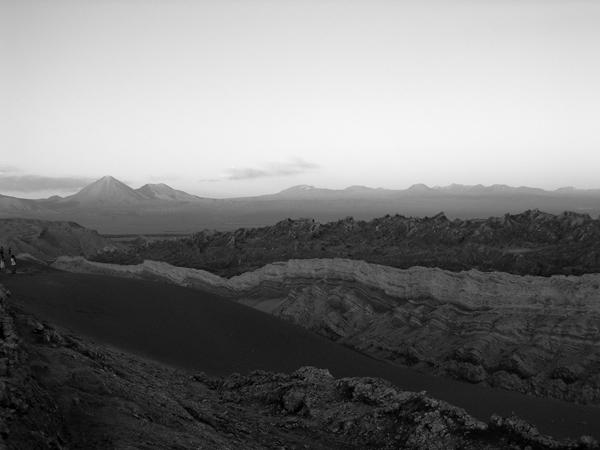
\includegraphics{grisvalleluna.jpg}
\caption{`grisvalleluna.jpg'}
\end{figure}

\begin{itemize}
\tightlist
\item
  seuillage avec un seuil de \(70\) :
\end{itemize}

\begin{figure}
\centering
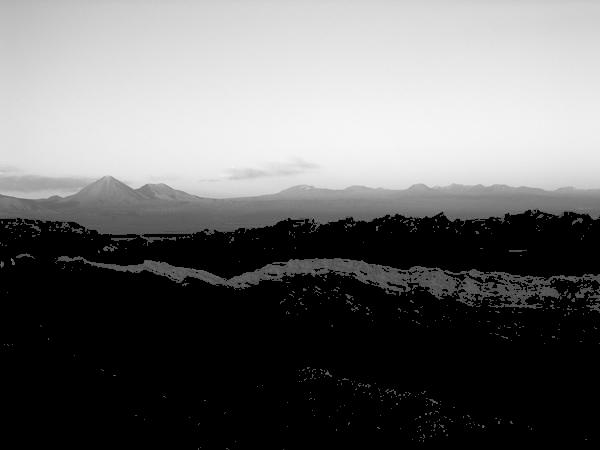
\includegraphics{seuil_70_grisvalleluna.jpg}
\caption{`seuil\_70\_grisvalleluna.jpg'}
\end{figure}

    \hypertarget{exercice-10-duxe9tection-de-contours}{%
\subsection{Exercice 10 : détection de
contours}\label{exercice-10-duxe9tection-de-contours}}

    \begin{Verbatim}[commandchars=\\\{\}]
{\color{incolor}In [{\color{incolor}94}]:} \PY{k}{def} \PY{n+nf}{contour}\PY{p}{(}\PY{n}{imsource}\PY{p}{,} \PY{n}{s}\PY{p}{)}\PY{p}{:}
             \PY{n}{im} \PY{o}{=} \PY{n}{Image}\PY{o}{.}\PY{n}{open}\PY{p}{(}\PY{n}{imsource}\PY{p}{)}
             \PY{n}{pixels} \PY{o}{=} \PY{n}{np}\PY{o}{.}\PY{n}{array}\PY{p}{(}\PY{n}{im}\PY{p}{)}
             \PY{n}{pixels} \PY{o}{=} \PY{n}{pixels}\PY{o}{.}\PY{n}{astype}\PY{p}{(}\PY{n+nb}{float}\PY{p}{)}
             \PY{k}{assert} \PY{n+nb}{len}\PY{p}{(}\PY{n}{pixels}\PY{o}{.}\PY{n}{shape}\PY{p}{)} \PY{o}{==} \PY{l+m+mi}{2}\PY{p}{,} \PY{l+s+s2}{\PYZdq{}}\PY{l+s+s2}{l}\PY{l+s+s2}{\PYZsq{}}\PY{l+s+s2}{image doit être en niveau de gris}\PY{l+s+s2}{\PYZdq{}}
             \PY{n}{hauteur}\PY{p}{,} \PY{n}{largeur} \PY{o}{=} \PY{n}{pixels}\PY{o}{.}\PY{n}{shape}\PY{p}{[}\PY{p}{:}\PY{l+m+mi}{2}\PY{p}{]}
             \PY{n}{pixels\PYZus{}res} \PY{o}{=} \PY{n}{np}\PY{o}{.}\PY{n}{zeros}\PY{p}{(}\PY{p}{[}\PY{n}{hauteur}\PY{p}{,}\PY{n}{largeur}\PY{p}{]}\PY{p}{,} \PY{n}{dtype}\PY{o}{=}\PY{l+s+s2}{\PYZdq{}}\PY{l+s+s2}{uint8}\PY{l+s+s2}{\PYZdq{}}\PY{p}{)}
             \PY{k}{for} \PY{n}{i} \PY{o+ow}{in} \PY{n+nb}{range}\PY{p}{(}\PY{l+m+mi}{1}\PY{p}{,} \PY{n}{hauteur} \PY{o}{\PYZhy{}} \PY{l+m+mi}{1}\PY{p}{)}\PY{p}{:}
                 \PY{k}{for} \PY{n}{j} \PY{o+ow}{in} \PY{n+nb}{range}\PY{p}{(}\PY{l+m+mi}{1}\PY{p}{,} \PY{n}{largeur} \PY{o}{\PYZhy{}} \PY{l+m+mi}{1}\PY{p}{)}\PY{p}{:}            
                     \PY{n}{a} \PY{o}{=} \PY{n}{pixels}\PY{p}{[}\PY{n}{i}\PY{p}{,} \PY{n}{j} \PY{o}{\PYZhy{}} \PY{l+m+mi}{1}\PY{p}{]}
                     \PY{n}{b} \PY{o}{=} \PY{n}{pixels}\PY{p}{[}\PY{n}{i}\PY{p}{,} \PY{n}{j} \PY{o}{+} \PY{l+m+mi}{1}\PY{p}{]}
                     \PY{n}{c} \PY{o}{=} \PY{n}{pixels}\PY{p}{[}\PY{n}{i} \PY{o}{\PYZhy{}} \PY{l+m+mi}{1}\PY{p}{,} \PY{n}{j}\PY{p}{]}
                     \PY{n}{d} \PY{o}{=} \PY{n}{pixels}\PY{p}{[}\PY{n}{i} \PY{o}{+} \PY{l+m+mi}{1}\PY{p}{,} \PY{n}{j}\PY{p}{]}
                     \PY{k}{if} \PY{n}{np}\PY{o}{.}\PY{n}{sqrt}\PY{p}{(}\PY{p}{(}\PY{n}{a} \PY{o}{\PYZhy{}} \PY{n}{b}\PY{p}{)} \PY{o}{*}\PY{o}{*} \PY{l+m+mi}{2} \PY{o}{+} \PY{p}{(}\PY{n}{c} \PY{o}{\PYZhy{}} \PY{n}{d}\PY{p}{)} \PY{o}{*}\PY{o}{*} \PY{l+m+mi}{2}\PY{p}{)} \PY{o}{\PYZlt{}}\PY{o}{=} \PY{n}{s}\PY{p}{:}
                         \PY{n}{pixels\PYZus{}res}\PY{p}{[}\PY{n}{i}\PY{p}{,} \PY{n}{j}\PY{p}{]} \PY{o}{=} \PY{l+m+mi}{255}
                     \PY{k}{else}\PY{p}{:}
                         \PY{n}{pixels\PYZus{}res}\PY{p}{[}\PY{n}{i}\PY{p}{,}\PY{n}{j}\PY{p}{]} \PY{o}{=} \PY{l+m+mi}{0}               
             \PY{n}{img\PYZus{}res} \PY{o}{=} \PY{n}{Image}\PY{o}{.}\PY{n}{fromarray}\PY{p}{(}\PY{n}{pixels\PYZus{}res}\PY{p}{)}
             \PY{n}{img\PYZus{}res}\PY{o}{.}\PY{n}{save}\PY{p}{(}\PY{l+s+s2}{\PYZdq{}}\PY{l+s+s2}{contour\PYZus{}}\PY{l+s+s2}{\PYZdq{}} \PY{o}{+} \PY{n+nb}{str}\PY{p}{(}\PY{n}{s}\PY{p}{)} \PY{o}{+} \PY{l+s+s2}{\PYZdq{}}\PY{l+s+s2}{\PYZus{}}\PY{l+s+s2}{\PYZdq{}} \PY{o}{+} \PY{n}{imsource}\PY{p}{)}
             \PY{n}{img\PYZus{}res}\PY{o}{.}\PY{n}{show}\PY{p}{(}\PY{p}{)}    
\end{Verbatim}


    \begin{Verbatim}[commandchars=\\\{\}]
{\color{incolor}In [{\color{incolor}97}]:} \PY{n}{contour}\PY{p}{(}\PY{l+s+s1}{\PYZsq{}}\PY{l+s+s1}{grisvalleluna.jpg}\PY{l+s+s1}{\PYZsq{}}\PY{p}{,} \PY{l+m+mi}{20}\PY{p}{)}
\end{Verbatim}


    \begin{itemize}
\tightlist
\item
  image initiale :
\end{itemize}

\begin{figure}
\centering
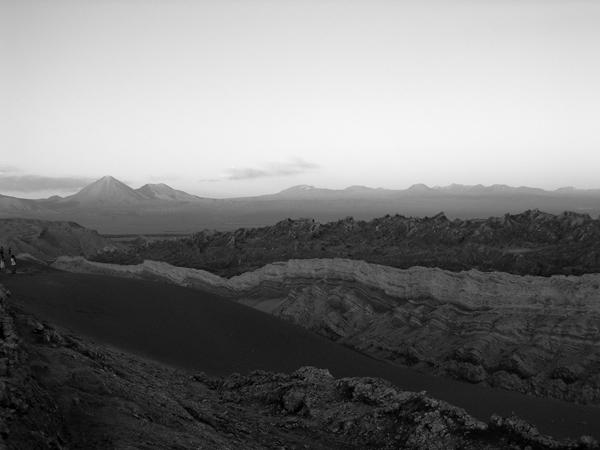
\includegraphics{grisvalleluna.jpg}
\caption{`grisvalleluna.jpg'}
\end{figure}

\begin{itemize}
\tightlist
\item
  contour avec un seuil de 5 pixels :
\end{itemize}

\begin{figure}
\centering
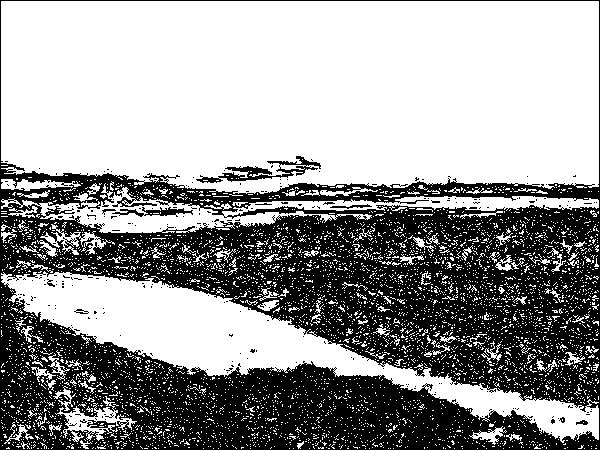
\includegraphics{contour_5_grisvalleluna.jpg}
\caption{`contour\_5\_grisvalleluna.jpg'}
\end{figure}

\begin{itemize}
\tightlist
\item
  contour avec un seuil de 10 pixels :
\end{itemize}

\begin{figure}
\centering
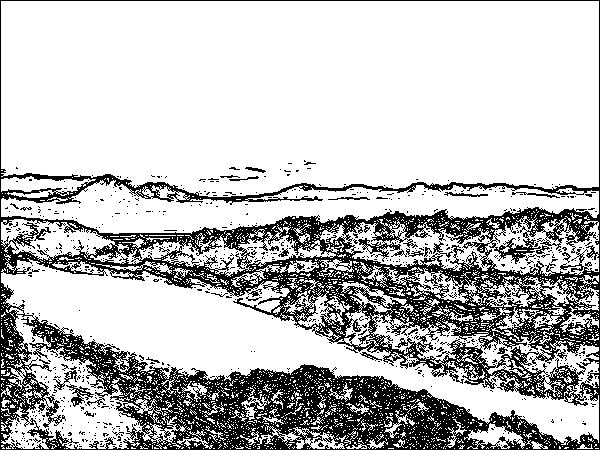
\includegraphics{contour_10_grisvalleluna.jpg}
\caption{`contour\_10\_grisvalleluna.jpg'}
\end{figure}

\begin{itemize}
\tightlist
\item
  contour avec un seuil de 20 pixels :
\end{itemize}

\begin{figure}
\centering
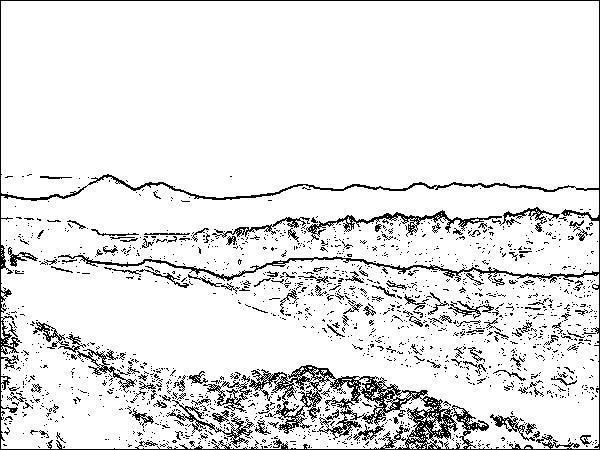
\includegraphics{contour_20_grisvalleluna.jpg}
\caption{`contour\_20\_grisvalleluna.jpg'}
\end{figure}

    \hypertarget{exercice-11-quart-de-tour-direct}{%
\subsection{\texorpdfstring{Exercice 11 \emph{Quart de tour
direct}}{Exercice 11 Quart de tour direct}}\label{exercice-11-quart-de-tour-direct}}

    \begin{Verbatim}[commandchars=\\\{\}]
{\color{incolor}In [{\color{incolor}110}]:} \PY{k}{def} \PY{n+nf}{quart\PYZus{}tour}\PY{p}{(}\PY{n}{fichier}\PY{p}{)}\PY{p}{:}
              \PY{n}{im}\PY{o}{=}\PY{n}{Image}\PY{o}{.}\PY{n}{open}\PY{p}{(}\PY{n}{fichier}\PY{p}{)}
              \PY{n}{pixels} \PY{o}{=} \PY{n}{np}\PY{o}{.}\PY{n}{array}\PY{p}{(}\PY{n}{im}\PY{p}{)}   
              \PY{k}{assert} \PY{n+nb}{len}\PY{p}{(}\PY{n}{pixels}\PY{o}{.}\PY{n}{shape}\PY{p}{)} \PY{o}{==} \PY{l+m+mi}{2} \PY{o+ow}{or} \PY{n+nb}{len}\PY{p}{(}\PY{n}{pixels}\PY{o}{.}\PY{n}{shape}\PY{p}{)} \PY{o}{==} \PY{l+m+mi}{3}\PY{p}{,} \PY{l+s+s2}{\PYZdq{}}\PY{l+s+s2}{format d}\PY{l+s+s2}{\PYZsq{}}\PY{l+s+s2}{image non conforme}\PY{l+s+s2}{\PYZdq{}}
              \PY{n}{hauteur}\PY{p}{,} \PY{n}{largeur} \PY{o}{=} \PY{n}{pixels}\PY{o}{.}\PY{n}{shape}\PY{p}{[}\PY{p}{:}\PY{l+m+mi}{2}\PY{p}{]}
              \PY{k}{if} \PY{n+nb}{len}\PY{p}{(}\PY{n}{pixels}\PY{o}{.}\PY{n}{shape}\PY{p}{)} \PY{o}{==} \PY{l+m+mi}{3}\PY{p}{:}
                  \PY{n}{pixels\PYZus{}res} \PY{o}{=} \PY{n}{np}\PY{o}{.}\PY{n}{zeros}\PY{p}{(}\PY{p}{[}\PY{n}{largeur}\PY{p}{,} \PY{n}{hauteur}\PY{p}{,} \PY{l+m+mi}{3}\PY{p}{]}\PY{p}{,} \PY{n}{dtype}\PY{o}{=}\PY{l+s+s2}{\PYZdq{}}\PY{l+s+s2}{uint8}\PY{l+s+s2}{\PYZdq{}}\PY{p}{)}
              \PY{k}{else}\PY{p}{:}
                  \PY{n}{pixels\PYZus{}res} \PY{o}{=} \PY{n}{np}\PY{o}{.}\PY{n}{zeros}\PY{p}{(}\PY{p}{[}\PY{n}{largeur}\PY{p}{,} \PY{n}{hauteur}\PY{p}{]}\PY{p}{,} \PY{n}{dtype}\PY{o}{=}\PY{l+s+s2}{\PYZdq{}}\PY{l+s+s2}{uint8}\PY{l+s+s2}{\PYZdq{}}\PY{p}{)}
              \PY{k}{for} \PY{n}{i} \PY{o+ow}{in} \PY{n+nb}{range}\PY{p}{(}\PY{n}{largeur}\PY{p}{)}\PY{p}{:}
                  \PY{k}{for} \PY{n}{j} \PY{o+ow}{in} \PY{n+nb}{range}\PY{p}{(}\PY{n}{hauteur}\PY{p}{)}\PY{p}{:}
                      \PY{n}{pixels\PYZus{}res}\PY{p}{[}\PY{n}{i}\PY{p}{,} \PY{n}{j}\PY{p}{]} \PY{o}{=} \PY{n}{pixels}\PY{p}{[}\PY{n}{j}\PY{p}{,} \PY{n}{largeur} \PY{o}{\PYZhy{}} \PY{l+m+mi}{1} \PY{o}{\PYZhy{}} \PY{n}{i}\PY{p}{]}
              \PY{n}{img\PYZus{}res} \PY{o}{=} \PY{n}{Image}\PY{o}{.}\PY{n}{fromarray}\PY{p}{(}\PY{n}{pixels\PYZus{}res}\PY{p}{)}
              \PY{n}{img\PYZus{}res}\PY{o}{.}\PY{n}{save}\PY{p}{(}\PY{l+s+s2}{\PYZdq{}}\PY{l+s+s2}{quart\PYZus{}tour\PYZus{}}\PY{l+s+s2}{\PYZdq{}} \PY{o}{+} \PY{n}{fichier}\PY{p}{)}
              \PY{n}{img\PYZus{}res}\PY{o}{.}\PY{n}{show}\PY{p}{(}\PY{p}{)}
\end{Verbatim}


    \begin{Verbatim}[commandchars=\\\{\}]
{\color{incolor}In [{\color{incolor}108}]:} \PY{n}{quart\PYZus{}tour}\PY{p}{(}\PY{l+s+s1}{\PYZsq{}}\PY{l+s+s1}{valleluna.jpg}\PY{l+s+s1}{\PYZsq{}}\PY{p}{)}
\end{Verbatim}


    \begin{itemize}
\tightlist
\item
  L'image initiale :
\end{itemize}

\begin{figure}
\centering
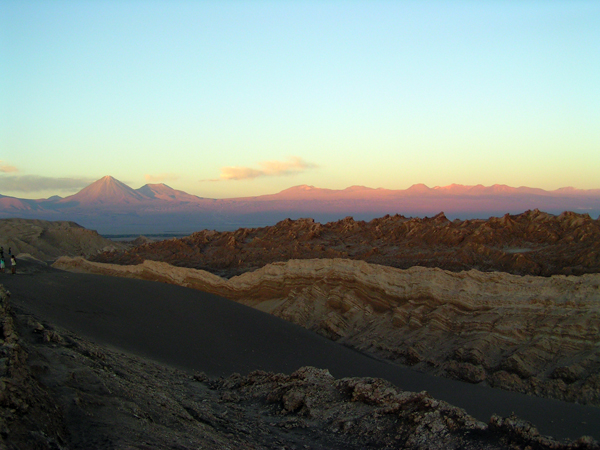
\includegraphics{valleluna.jpg}
\caption{`valleluna.jpg'}
\end{figure}

\begin{itemize}
\tightlist
\item
  L'image obtenue par quart de tour direct :
\end{itemize}

\begin{figure}
\centering
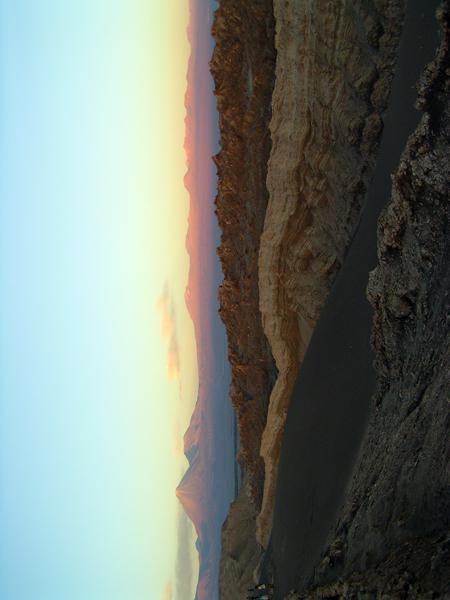
\includegraphics{quart_tour_valleluna.jpg}
\caption{`quart\_tour\_valleluna.jpg'}
\end{figure}

    \hypertarget{exercice-12-ruxe9duction-agrandissement}{%
\subsection{\texorpdfstring{Exercice 12 \emph{Réduction /
Agrandissement}}{Exercice 12 Réduction / Agrandissement}}\label{exercice-12-ruxe9duction-agrandissement}}

    \begin{Verbatim}[commandchars=\\\{\}]
{\color{incolor}In [{\color{incolor}113}]:} \PY{k}{def} \PY{n+nf}{reduction}\PY{p}{(}\PY{n}{imsource}\PY{p}{,} \PY{n}{coef}\PY{p}{)}\PY{p}{:}
              \PY{n}{im} \PY{o}{=} \PY{n}{Image}\PY{o}{.}\PY{n}{open}\PY{p}{(}\PY{n}{imsource}\PY{p}{)}
              \PY{n}{pixels} \PY{o}{=} \PY{n}{np}\PY{o}{.}\PY{n}{array}\PY{p}{(}\PY{n}{im}\PY{p}{)}   
              \PY{k}{assert} \PY{n+nb}{len}\PY{p}{(}\PY{n}{pixels}\PY{o}{.}\PY{n}{shape}\PY{p}{)} \PY{o}{==} \PY{l+m+mi}{2} \PY{o+ow}{or} \PY{n+nb}{len}\PY{p}{(}\PY{n}{pixels}\PY{o}{.}\PY{n}{shape}\PY{p}{)} \PY{o}{==} \PY{l+m+mi}{3}\PY{p}{,} \PY{l+s+s2}{\PYZdq{}}\PY{l+s+s2}{format d}\PY{l+s+s2}{\PYZsq{}}\PY{l+s+s2}{image non conforme}\PY{l+s+s2}{\PYZdq{}}
              \PY{n}{hauteur}\PY{p}{,} \PY{n}{largeur} \PY{o}{=} \PY{n}{pixels}\PY{o}{.}\PY{n}{shape}\PY{p}{[}\PY{p}{:}\PY{l+m+mi}{2}\PY{p}{]}
              \PY{n}{hauteur\PYZus{}res}\PY{p}{,} \PY{n}{largeur\PYZus{}res} \PY{o}{=} \PY{n}{hauteur} \PY{o}{/}\PY{o}{/} \PY{n}{coef}\PY{p}{,} \PY{n}{largeur} \PY{o}{/}\PY{o}{/} \PY{n}{coef}
              \PY{n}{pixels\PYZus{}res} \PY{o}{=} \PY{n}{np}\PY{o}{.}\PY{n}{zeros}\PY{p}{(}\PY{p}{[}\PY{n}{hauteur\PYZus{}res}\PY{p}{,} \PY{n}{largeur\PYZus{}res}\PY{p}{,} \PY{l+m+mi}{3}\PY{p}{]}\PY{p}{,} \PY{n}{dtype}\PY{o}{=}\PY{l+s+s2}{\PYZdq{}}\PY{l+s+s2}{uint8}\PY{l+s+s2}{\PYZdq{}}\PY{p}{)}    
              \PY{k}{for} \PY{n}{i} \PY{o+ow}{in} \PY{n+nb}{range}\PY{p}{(}\PY{n}{hauteur\PYZus{}res}\PY{p}{)}\PY{p}{:}
                  \PY{k}{for} \PY{n}{j} \PY{o+ow}{in} \PY{n+nb}{range}\PY{p}{(}\PY{n}{largeur\PYZus{}res}\PY{p}{)}\PY{p}{:}
                      \PY{n}{pixels\PYZus{}res}\PY{p}{[}\PY{n}{i}\PY{p}{,} \PY{n}{j}\PY{p}{]} \PY{o}{=} \PY{n}{pixels}\PY{p}{[}\PY{n}{i} \PY{o}{*} \PY{n}{coef}\PY{p}{,} \PY{n}{j} \PY{o}{*} \PY{n}{coef}\PY{p}{]}
              \PY{n}{img\PYZus{}res} \PY{o}{=} \PY{n}{Image}\PY{o}{.}\PY{n}{fromarray}\PY{p}{(}\PY{n}{pixels\PYZus{}res}\PY{p}{)}
              \PY{n}{img\PYZus{}res}\PY{o}{.}\PY{n}{save}\PY{p}{(}\PY{l+s+s2}{\PYZdq{}}\PY{l+s+s2}{reduction\PYZus{}}\PY{l+s+s2}{\PYZdq{}} \PY{o}{+} \PY{n+nb}{str}\PY{p}{(}\PY{n}{coef}\PY{p}{)} \PY{o}{+} \PY{l+s+s2}{\PYZdq{}}\PY{l+s+s2}{\PYZus{}}\PY{l+s+s2}{\PYZdq{}} \PY{o}{+} \PY{n}{imsource}\PY{p}{)}
              \PY{n}{img\PYZus{}res}\PY{o}{.}\PY{n}{show}\PY{p}{(}\PY{p}{)}
\end{Verbatim}


    \begin{Verbatim}[commandchars=\\\{\}]
{\color{incolor}In [{\color{incolor}114}]:} \PY{n}{reduction}\PY{p}{(}\PY{l+s+s2}{\PYZdq{}}\PY{l+s+s2}{valleluna.jpg}\PY{l+s+s2}{\PYZdq{}}\PY{p}{,} \PY{l+m+mi}{2}\PY{p}{)}
\end{Verbatim}


    \begin{itemize}
\tightlist
\item
  L'image initiale :
\end{itemize}

\begin{figure}
\centering
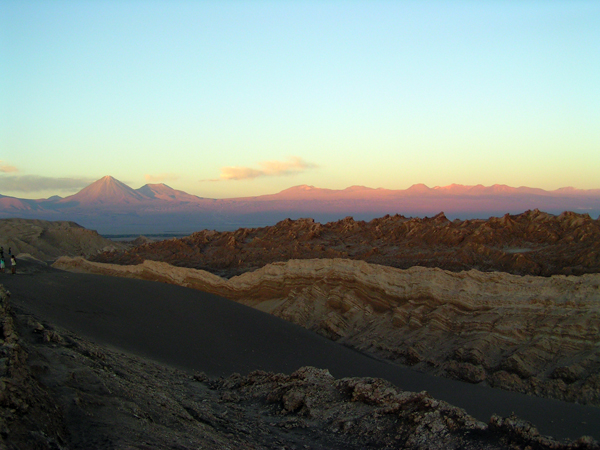
\includegraphics{valleluna.jpg}
\caption{`valleluna.jpg'}
\end{figure}

\begin{itemize}
\tightlist
\item
  L'image obtenue par réduction de coefficient 2 :
\end{itemize}

\begin{figure}
\centering
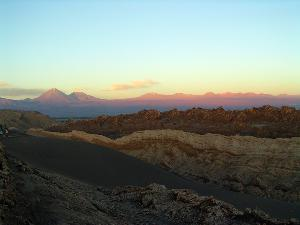
\includegraphics{reduction_2_valleluna.jpg}
\caption{`reduction\_2\_valleluna.jpg'}
\end{figure}

    \begin{Verbatim}[commandchars=\\\{\}]
{\color{incolor}In [{\color{incolor}121}]:} \PY{k}{def} \PY{n+nf}{agrandissement}\PY{p}{(}\PY{n}{imsource}\PY{p}{,} \PY{n}{coef}\PY{p}{)}\PY{p}{:}
              \PY{n}{im} \PY{o}{=} \PY{n}{Image}\PY{o}{.}\PY{n}{open}\PY{p}{(}\PY{n}{imsource}\PY{p}{)}
              \PY{n}{pixels} \PY{o}{=} \PY{n}{np}\PY{o}{.}\PY{n}{array}\PY{p}{(}\PY{n}{im}\PY{p}{)}   
              \PY{k}{assert} \PY{n+nb}{len}\PY{p}{(}\PY{n}{pixels}\PY{o}{.}\PY{n}{shape}\PY{p}{)} \PY{o}{==} \PY{l+m+mi}{2} \PY{o+ow}{or} \PY{n+nb}{len}\PY{p}{(}\PY{n}{pixels}\PY{o}{.}\PY{n}{shape}\PY{p}{)} \PY{o}{==} \PY{l+m+mi}{3}\PY{p}{,} \PY{l+s+s2}{\PYZdq{}}\PY{l+s+s2}{format d}\PY{l+s+s2}{\PYZsq{}}\PY{l+s+s2}{image non conforme}\PY{l+s+s2}{\PYZdq{}}
              \PY{n}{hauteur}\PY{p}{,} \PY{n}{largeur} \PY{o}{=} \PY{n}{pixels}\PY{o}{.}\PY{n}{shape}\PY{p}{[}\PY{p}{:}\PY{l+m+mi}{2}\PY{p}{]}
              \PY{n}{hauteur\PYZus{}res}\PY{p}{,} \PY{n}{largeur\PYZus{}res} \PY{o}{=} \PY{n}{hauteur} \PY{o}{*} \PY{n}{coef}\PY{p}{,} \PY{n}{largeur} \PY{o}{*} \PY{n}{coef}
              \PY{n}{pixels\PYZus{}res} \PY{o}{=} \PY{n}{np}\PY{o}{.}\PY{n}{zeros}\PY{p}{(}\PY{p}{[}\PY{n}{hauteur\PYZus{}res}\PY{p}{,} \PY{n}{largeur\PYZus{}res}\PY{p}{,} \PY{l+m+mi}{3}\PY{p}{]}\PY{p}{,} \PY{n}{dtype}\PY{o}{=}\PY{l+s+s2}{\PYZdq{}}\PY{l+s+s2}{uint8}\PY{l+s+s2}{\PYZdq{}}\PY{p}{)}    
              \PY{k}{for} \PY{n}{i} \PY{o+ow}{in} \PY{n+nb}{range}\PY{p}{(}\PY{n}{hauteur\PYZus{}res}\PY{p}{)}\PY{p}{:}
                  \PY{k}{for} \PY{n}{j} \PY{o+ow}{in} \PY{n+nb}{range}\PY{p}{(}\PY{n}{largeur\PYZus{}res}\PY{p}{)}\PY{p}{:}
                      \PY{n}{pixels\PYZus{}res}\PY{p}{[}\PY{n}{i}\PY{p}{,} \PY{n}{j}\PY{p}{]} \PY{o}{=} \PY{n}{pixels}\PY{p}{[}\PY{n}{i} \PY{o}{/}\PY{o}{/} \PY{n}{coef}\PY{p}{,} \PY{n}{j} \PY{o}{/}\PY{o}{/} \PY{n}{coef}\PY{p}{]}
              \PY{n}{img\PYZus{}res} \PY{o}{=} \PY{n}{Image}\PY{o}{.}\PY{n}{fromarray}\PY{p}{(}\PY{n}{pixels\PYZus{}res}\PY{p}{)}
              \PY{n}{img\PYZus{}res}\PY{o}{.}\PY{n}{save}\PY{p}{(}\PY{l+s+s2}{\PYZdq{}}\PY{l+s+s2}{agrandissement\PYZus{}}\PY{l+s+s2}{\PYZdq{}} \PY{o}{+} \PY{n+nb}{str}\PY{p}{(}\PY{n}{coef}\PY{p}{)} \PY{o}{+} \PY{l+s+s2}{\PYZdq{}}\PY{l+s+s2}{\PYZus{}}\PY{l+s+s2}{\PYZdq{}} \PY{o}{+} \PY{n}{imsource}\PY{p}{)}
              \PY{n}{img\PYZus{}res}\PY{o}{.}\PY{n}{show}\PY{p}{(}\PY{p}{)}
\end{Verbatim}


    \begin{Verbatim}[commandchars=\\\{\}]
{\color{incolor}In [{\color{incolor}122}]:} \PY{n}{agrandissement}\PY{p}{(}\PY{l+s+s2}{\PYZdq{}}\PY{l+s+s2}{valleluna.jpg}\PY{l+s+s2}{\PYZdq{}}\PY{p}{,} \PY{l+m+mi}{2}\PY{p}{)}
\end{Verbatim}


    \begin{Verbatim}[commandchars=\\\{\}]
{\color{incolor}In [{\color{incolor}123}]:} \PY{n}{reduction}\PY{p}{(}\PY{l+s+s2}{\PYZdq{}}\PY{l+s+s2}{valleluna.jpg}\PY{l+s+s2}{\PYZdq{}}\PY{p}{,} \PY{l+m+mi}{2}\PY{p}{)}
          \PY{n}{agrandissement}\PY{p}{(}\PY{l+s+s2}{\PYZdq{}}\PY{l+s+s2}{reduction\PYZus{}2\PYZus{}valleluna.jpg}\PY{l+s+s2}{\PYZdq{}}\PY{p}{,} \PY{l+m+mi}{4}\PY{p}{)}
\end{Verbatim}


    \begin{itemize}
\tightlist
\item
  L'image initiale :
\end{itemize}

\begin{figure}
\centering
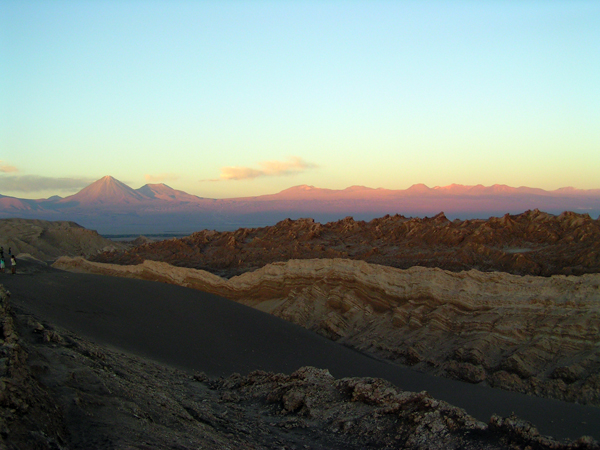
\includegraphics{valleluna.jpg}
\caption{`valleluna.jpg'}
\end{figure}

\begin{itemize}
\tightlist
\item
  L'image obtenue par agrandissement de coefficient 2 :
\end{itemize}

\begin{figure}
\centering
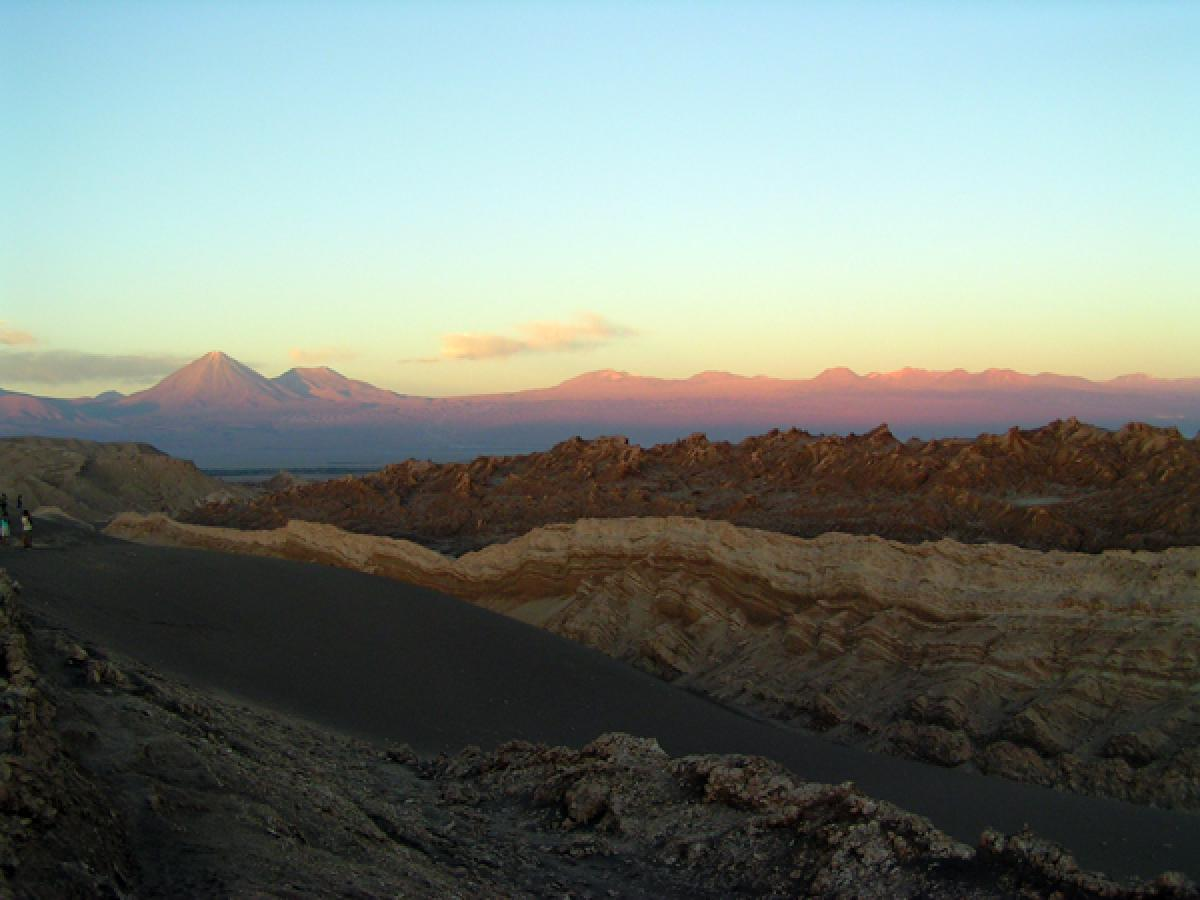
\includegraphics{agrandissement_2_valleluna.jpg}
\caption{`agrandissement\_2\_valleluna.jpg'}
\end{figure}

\begin{itemize}
\tightlist
\item
  L'image obtenue par réduction de coefficient 2 puis agrandissement de
  coefficient 4 :
\end{itemize}

\begin{figure}
\centering
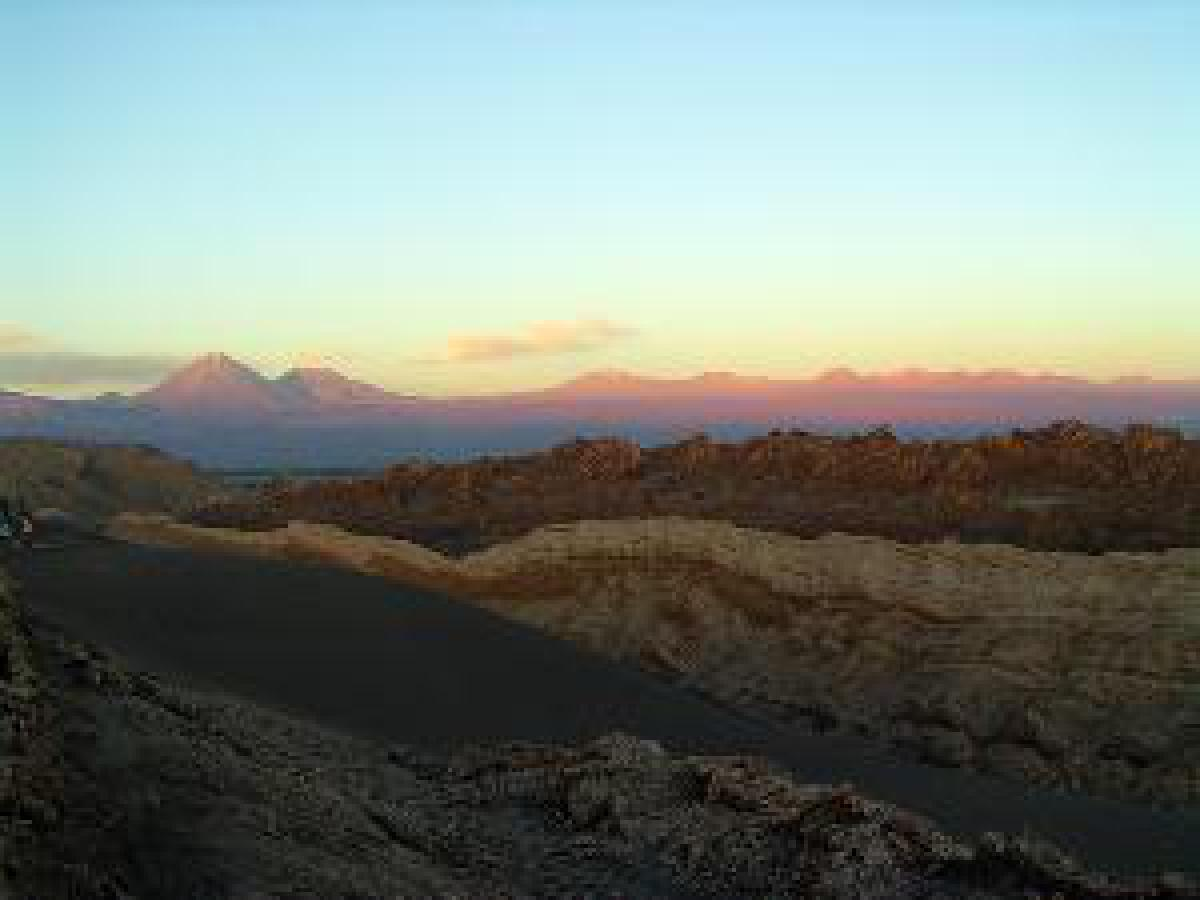
\includegraphics{agrandissement_4_reduction_2_valleluna.jpg}
\caption{`agrandissement\_4\_reduction\_2\_valleluna.jpg'}
\end{figure}

    \hypertarget{exercice-13-stuxe9ganographie}{%
\subsection{\texorpdfstring{Exercice 13
\emph{Stéganographie}}{Exercice 13 Stéganographie}}\label{exercice-13-stuxe9ganographie}}

    \begin{Verbatim}[commandchars=\\\{\}]
{\color{incolor}In [{\color{incolor}144}]:} \PY{k}{def} \PY{n+nf}{extraction\PYZus{}image}\PY{p}{(}\PY{n}{imsource}\PY{p}{)}\PY{p}{:}
              \PY{l+s+sd}{\PYZdq{}\PYZdq{}\PYZdq{}Extrait une image cachée dans imsource :  les 4 bits de poids forts}
          \PY{l+s+sd}{    de l\PYZsq{}image cachée sont les 4 bits de poids faibles dans imsource\PYZdq{}\PYZdq{}\PYZdq{}}
              \PY{n}{im} \PY{o}{=} \PY{n}{Image}\PY{o}{.}\PY{n}{open}\PY{p}{(}\PY{n}{imsource}\PY{p}{)}
              \PY{n}{pixels} \PY{o}{=} \PY{n}{np}\PY{o}{.}\PY{n}{array}\PY{p}{(}\PY{n}{im}\PY{p}{)}   
              \PY{k}{assert} \PY{n+nb}{len}\PY{p}{(}\PY{n}{pixels}\PY{o}{.}\PY{n}{shape}\PY{p}{)} \PY{o}{==} \PY{l+m+mi}{2} \PY{p}{,} \PY{l+s+s2}{\PYZdq{}}\PY{l+s+s2}{Il faut une image en niveau de gris}\PY{l+s+s2}{\PYZdq{}}
              \PY{n}{pixels\PYZus{}res} \PY{o}{=} \PY{n}{np}\PY{o}{.}\PY{n}{zeros\PYZus{}like}\PY{p}{(}\PY{n}{pixels}\PY{p}{)} 
              \PY{n}{hauteur}\PY{p}{,} \PY{n}{largeur} \PY{o}{=} \PY{n}{pixels}\PY{o}{.}\PY{n}{shape}\PY{p}{[}\PY{p}{:}\PY{l+m+mi}{2}\PY{p}{]}
              \PY{k}{for} \PY{n}{i} \PY{o+ow}{in} \PY{n+nb}{range}\PY{p}{(}\PY{n}{hauteur}\PY{p}{)}\PY{p}{:}
                  \PY{k}{for} \PY{n}{j} \PY{o+ow}{in} \PY{n+nb}{range}\PY{p}{(}\PY{n}{largeur}\PY{p}{)}\PY{p}{:}
                      \PY{n}{pixels\PYZus{}res}\PY{p}{[}\PY{n}{i}\PY{p}{,} \PY{n}{j}\PY{p}{]} \PY{o}{=} \PY{p}{(}\PY{n}{pixels}\PY{p}{[}\PY{n}{i}\PY{p}{,} \PY{n}{j} \PY{p}{]} \PY{o}{\PYZpc{}} \PY{l+m+mi}{16}\PY{p}{)} \PY{o}{*} \PY{l+m+mi}{16}
              \PY{n}{img\PYZus{}res} \PY{o}{=} \PY{n}{Image}\PY{o}{.}\PY{n}{fromarray}\PY{p}{(}\PY{n}{pixels\PYZus{}res}\PY{p}{)}
              \PY{n}{img\PYZus{}res}\PY{o}{.}\PY{n}{save}\PY{p}{(}\PY{l+s+s2}{\PYZdq{}}\PY{l+s+s2}{image\PYZus{}cache\PYZus{}}\PY{l+s+s2}{\PYZdq{}}  \PY{o}{+} \PY{n}{imsource}\PY{p}{)}
              \PY{n}{img\PYZus{}res}\PY{o}{.}\PY{n}{show}\PY{p}{(}\PY{p}{)}
\end{Verbatim}


    \begin{Verbatim}[commandchars=\\\{\}]
{\color{incolor}In [{\color{incolor}127}]:} \PY{n}{extraction\PYZus{}image}\PY{p}{(}\PY{l+s+s2}{\PYZdq{}}\PY{l+s+s2}{mystere.png}\PY{l+s+s2}{\PYZdq{}}\PY{p}{)}
\end{Verbatim}


    \begin{itemize}
\tightlist
\item
  L'image source :
\end{itemize}

\begin{figure}
\centering
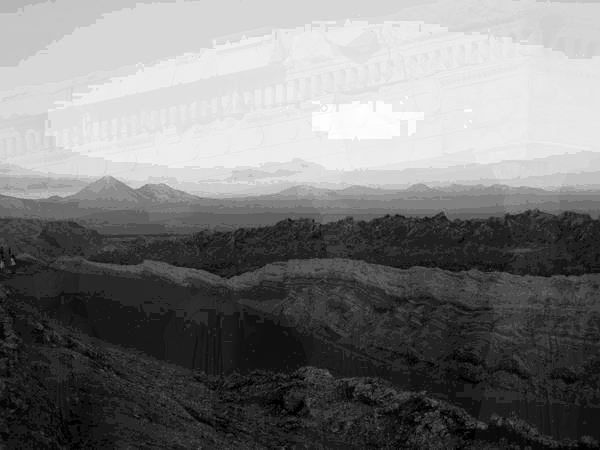
\includegraphics{mystere.png}
\caption{`mystere.png'}
\end{figure}

\begin{itemize}
\tightlist
\item
  L'image qui était cachée dans l'image source :
\end{itemize}

\begin{figure}
\centering
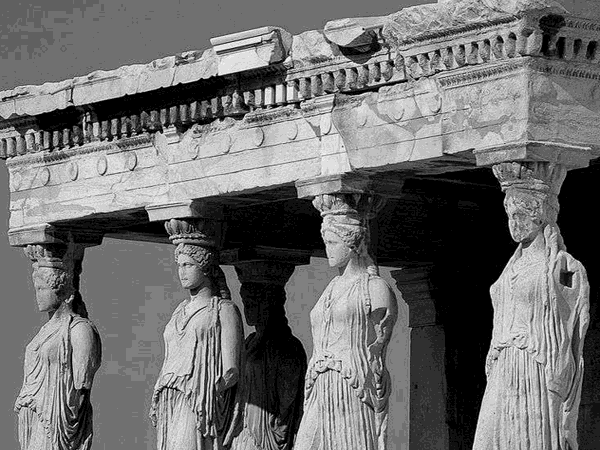
\includegraphics{image_cache_mystere.png}
\caption{'image\_cache\_\_mystere.png'}
\end{figure}

    \begin{Verbatim}[commandchars=\\\{\}]
{\color{incolor}In [{\color{incolor}131}]:} \PY{k}{def} \PY{n+nf}{cache\PYZus{}image}\PY{p}{(}\PY{n}{imcache}\PY{p}{,} \PY{n}{imsecret}\PY{p}{)}\PY{p}{:}
              \PY{l+s+sd}{\PYZdq{}\PYZdq{}\PYZdq{}Cache imsecret dans imcache  :  les 4 bits de poids forts de imsecret}
          \PY{l+s+sd}{    remplacent les 4 bits de poids faibles de  imcache\PYZdq{}\PYZdq{}\PYZdq{}}
              \PY{n}{im1} \PY{o}{=} \PY{n}{Image}\PY{o}{.}\PY{n}{open}\PY{p}{(}\PY{n}{imcache}\PY{p}{)}
              \PY{n}{im2} \PY{o}{=} \PY{n}{Image}\PY{o}{.}\PY{n}{open}\PY{p}{(}\PY{n}{imsecret}\PY{p}{)}
              \PY{n}{pixels1} \PY{o}{=} \PY{n}{np}\PY{o}{.}\PY{n}{array}\PY{p}{(}\PY{n}{im1}\PY{p}{)}
              \PY{n}{pixels2} \PY{o}{=} \PY{n}{np}\PY{o}{.}\PY{n}{array}\PY{p}{(}\PY{n}{im2}\PY{p}{)} 
              \PY{k}{assert} \PY{n+nb}{len}\PY{p}{(}\PY{n}{pixels1}\PY{o}{.}\PY{n}{shape}\PY{p}{)} \PY{o}{==} \PY{l+m+mi}{2} \PY{o+ow}{and}  \PY{n}{pixels1}\PY{o}{.}\PY{n}{shape} \PY{o}{==} \PY{n}{pixels2}\PY{o}{.}\PY{n}{shape}\PY{p}{,} \PY{l+s+s2}{\PYZdq{}}\PY{l+s+s2}{Il faut deux images en niveau de gris de même dimension}\PY{l+s+s2}{\PYZdq{}}
              \PY{n}{hauteur}\PY{p}{,} \PY{n}{largeur} \PY{o}{=} \PY{n}{pixels1}\PY{o}{.}\PY{n}{shape}\PY{p}{[}\PY{p}{:}\PY{l+m+mi}{2}\PY{p}{]}
              \PY{n}{pixels\PYZus{}res} \PY{o}{=} \PY{n}{np}\PY{o}{.}\PY{n}{zeros\PYZus{}like}\PY{p}{(}\PY{n}{pixels1}\PY{p}{)}
              \PY{k}{for} \PY{n}{i} \PY{o+ow}{in} \PY{n+nb}{range}\PY{p}{(}\PY{n}{hauteur}\PY{p}{)}\PY{p}{:}
                  \PY{k}{for} \PY{n}{j} \PY{o+ow}{in} \PY{n+nb}{range}\PY{p}{(}\PY{n}{largeur}\PY{p}{)}\PY{p}{:}
                      \PY{n}{pixels\PYZus{}res}\PY{p}{[}\PY{n}{i}\PY{p}{,} \PY{n}{j}\PY{p}{]} \PY{o}{=} \PY{p}{(}\PY{n}{pixels1}\PY{p}{[}\PY{n}{i}\PY{p}{,} \PY{n}{j}\PY{p}{]} \PY{o}{/}\PY{o}{/} \PY{l+m+mi}{16}\PY{p}{)} \PY{o}{*} \PY{l+m+mi}{16} \PY{o}{+} \PY{n}{pixels2}\PY{p}{[}\PY{n}{i}\PY{p}{,} \PY{n}{j}\PY{p}{]} \PY{o}{/}\PY{o}{/} \PY{l+m+mi}{16}
              \PY{n}{img\PYZus{}res} \PY{o}{=} \PY{n}{Image}\PY{o}{.}\PY{n}{fromarray}\PY{p}{(}\PY{n}{pixels\PYZus{}res}\PY{p}{)}
              \PY{n}{img\PYZus{}res}\PY{o}{.}\PY{n}{save}\PY{p}{(}\PY{l+s+s2}{\PYZdq{}}\PY{l+s+s2}{image\PYZus{}}\PY{l+s+s2}{\PYZdq{}} \PY{o}{+} \PY{n}{imsecret}\PY{o}{.}\PY{n}{split}\PY{p}{(}\PY{l+s+s1}{\PYZsq{}}\PY{l+s+s1}{.}\PY{l+s+s1}{\PYZsq{}}\PY{p}{)}\PY{p}{[}\PY{l+m+mi}{0}\PY{p}{]} \PY{o}{+} \PY{l+s+s2}{\PYZdq{}}\PY{l+s+s2}{\PYZus{}dans\PYZus{}}\PY{l+s+s2}{\PYZdq{}} \PY{o}{+}  \PY{n}{imcache}\PY{o}{.}\PY{n}{split}\PY{p}{(}\PY{l+s+s1}{\PYZsq{}}\PY{l+s+s1}{.}\PY{l+s+s1}{\PYZsq{}}\PY{p}{)}\PY{p}{[}\PY{l+m+mi}{0}\PY{p}{]} \PY{o}{+} \PY{l+s+s2}{\PYZdq{}}\PY{l+s+s2}{.png}\PY{l+s+s2}{\PYZdq{}}\PY{p}{)}
              \PY{n}{img\PYZus{}res}\PY{o}{.}\PY{n}{show}\PY{p}{(}\PY{p}{)}
\end{Verbatim}


    \begin{Verbatim}[commandchars=\\\{\}]
{\color{incolor}In [{\color{incolor}136}]:} \PY{n}{gris}\PY{p}{(}\PY{l+s+s1}{\PYZsq{}}\PY{l+s+s1}{cypres.bmp}\PY{l+s+s1}{\PYZsq{}}\PY{p}{,}\PY{p}{[}\PY{l+m+mi}{30}\PY{p}{,} \PY{l+m+mi}{59}\PY{p}{,} \PY{l+m+mi}{11}\PY{p}{]}\PY{p}{)}
\end{Verbatim}


    \begin{Verbatim}[commandchars=\\\{\}]
{\color{incolor}In [{\color{incolor}137}]:} \PY{n}{gris}\PY{p}{(}\PY{l+s+s1}{\PYZsq{}}\PY{l+s+s1}{femme.bmp}\PY{l+s+s1}{\PYZsq{}}\PY{p}{,}\PY{p}{[}\PY{l+m+mi}{30}\PY{p}{,} \PY{l+m+mi}{59}\PY{p}{,} \PY{l+m+mi}{11}\PY{p}{]}\PY{p}{)}
\end{Verbatim}


    \begin{Verbatim}[commandchars=\\\{\}]
{\color{incolor}In [{\color{incolor}138}]:} \PY{n}{cache\PYZus{}image}\PY{p}{(}\PY{l+s+s1}{\PYZsq{}}\PY{l+s+s1}{griscypres.bmp}\PY{l+s+s1}{\PYZsq{}}\PY{p}{,} \PY{l+s+s1}{\PYZsq{}}\PY{l+s+s1}{grisfemme.bmp}\PY{l+s+s1}{\PYZsq{}}\PY{p}{)}
\end{Verbatim}


    \begin{Verbatim}[commandchars=\\\{\}]
{\color{incolor}In [{\color{incolor}140}]:} \PY{n}{extraction\PYZus{}image\PYZus{}}\PY{p}{(}\PY{l+s+s2}{\PYZdq{}}\PY{l+s+s2}{image\PYZus{}grisfemme\PYZus{}dans\PYZus{}griscypres.png}\PY{l+s+s2}{\PYZdq{}}\PY{p}{)}
\end{Verbatim}


    \begin{itemize}
\tightlist
\item
  Image cachette avant stéganographie :
\end{itemize}

\begin{figure}
\centering
\includegraphics{griscypres.bmp}
\caption{`griscypres.bmp'}
\end{figure}

\begin{itemize}
\tightlist
\item
  Image secret / cachée avant stéganographie :
\end{itemize}

\begin{figure}
\centering
\includegraphics{grisfemme.bmp}
\caption{`grisfemme.bmp'}
\end{figure}

\begin{itemize}
\tightlist
\item
  Image cachette avec stéganographie :
\end{itemize}

\begin{figure}
\centering
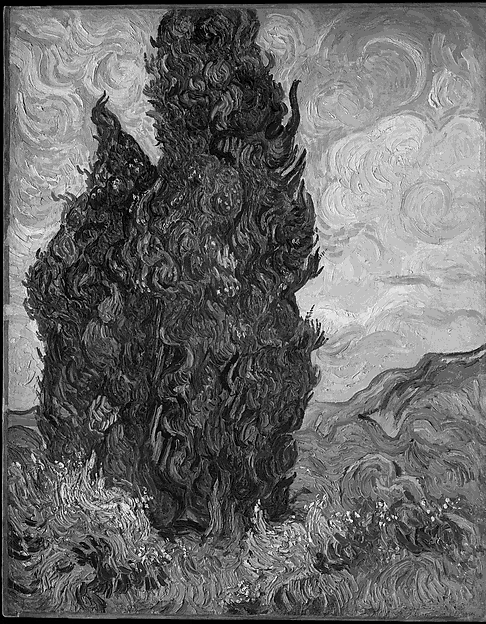
\includegraphics{image_grisfemme_dans_griscypres.png}
\caption{`image\_grisfemme\_dans\_griscypres.png'}
\end{figure}

\begin{itemize}
\tightlist
\item
  Image secret / cachée extraite après stéganographie :
\end{itemize}

\begin{figure}
\centering
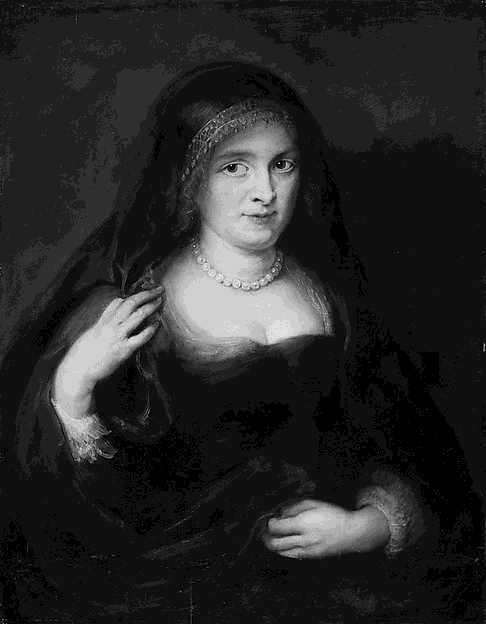
\includegraphics{image_cache_image_grisfemme_dans_griscypres.png}
\caption{`image\_cache\_image\_grisfemme\_dans\_griscypres.png'}
\end{figure}

    \begin{Verbatim}[commandchars=\\\{\}]
{\color{incolor}In [{\color{incolor}145}]:} \PY{k}{def} \PY{n+nf}{extraction\PYZus{}image\PYZus{}couleur}\PY{p}{(}\PY{n}{imsource}\PY{p}{)}\PY{p}{:}
              \PY{l+s+sd}{\PYZdq{}\PYZdq{}\PYZdq{}Extrait une image cachée dans imsource :  les 4 bits de poids forts}
          \PY{l+s+sd}{    de l\PYZsq{}image cachée sont les 4 bits de poids faibles dans imsource\PYZdq{}\PYZdq{}\PYZdq{}}
              \PY{n}{im} \PY{o}{=} \PY{n}{Image}\PY{o}{.}\PY{n}{open}\PY{p}{(}\PY{n}{imsource}\PY{p}{)}
              \PY{n}{pixels} \PY{o}{=} \PY{n}{np}\PY{o}{.}\PY{n}{array}\PY{p}{(}\PY{n}{im}\PY{p}{)}   
              \PY{k}{assert} \PY{n+nb}{len}\PY{p}{(}\PY{n}{pixels}\PY{o}{.}\PY{n}{shape}\PY{p}{)} \PY{o}{==} \PY{l+m+mi}{3}\PY{p}{,} \PY{l+s+s2}{\PYZdq{}}\PY{l+s+s2}{Il faut une image en R,G,B)}\PY{l+s+s2}{\PYZdq{}}
              \PY{n}{pixels\PYZus{}res} \PY{o}{=} \PY{n}{np}\PY{o}{.}\PY{n}{zeros\PYZus{}like}\PY{p}{(}\PY{n}{pixels}\PY{p}{)} 
              \PY{n}{hauteur}\PY{p}{,} \PY{n}{largeur} \PY{o}{=} \PY{n}{pixels}\PY{o}{.}\PY{n}{shape}\PY{p}{[}\PY{p}{:}\PY{l+m+mi}{2}\PY{p}{]}
              \PY{k}{for} \PY{n}{i} \PY{o+ow}{in} \PY{n+nb}{range}\PY{p}{(}\PY{n}{hauteur}\PY{p}{)}\PY{p}{:}
                  \PY{k}{for} \PY{n}{j} \PY{o+ow}{in} \PY{n+nb}{range}\PY{p}{(}\PY{n}{largeur}\PY{p}{)}\PY{p}{:}
                      \PY{k}{for} \PY{n}{k} \PY{o+ow}{in} \PY{n+nb}{range}\PY{p}{(}\PY{l+m+mi}{3}\PY{p}{)}\PY{p}{:}
                          \PY{n}{pixels\PYZus{}res}\PY{p}{[}\PY{n}{i}\PY{p}{,} \PY{n}{j}\PY{p}{,} \PY{n}{k}\PY{p}{]} \PY{o}{=} \PY{p}{(}\PY{n}{pixels}\PY{p}{[}\PY{n}{i}\PY{p}{,} \PY{n}{j}\PY{p}{,} \PY{n}{k}\PY{p}{]} \PY{o}{\PYZpc{}} \PY{l+m+mi}{16}\PY{p}{)} \PY{o}{*} \PY{l+m+mi}{16}
              \PY{n}{img\PYZus{}res} \PY{o}{=} \PY{n}{Image}\PY{o}{.}\PY{n}{fromarray}\PY{p}{(}\PY{n}{pixels\PYZus{}res}\PY{p}{)}
              \PY{n}{img\PYZus{}res}\PY{o}{.}\PY{n}{save}\PY{p}{(}\PY{l+s+s2}{\PYZdq{}}\PY{l+s+s2}{image\PYZus{}cache\PYZus{}}\PY{l+s+s2}{\PYZdq{}}  \PY{o}{+} \PY{n}{imsource}\PY{p}{)}
              \PY{n}{img\PYZus{}res}\PY{o}{.}\PY{n}{show}\PY{p}{(}\PY{p}{)}
          
          \PY{k}{def} \PY{n+nf}{cache\PYZus{}image\PYZus{}couleur}\PY{p}{(}\PY{n}{imcache}\PY{p}{,} \PY{n}{imsecret}\PY{p}{)}\PY{p}{:}
              \PY{l+s+sd}{\PYZdq{}\PYZdq{}\PYZdq{}Cache imsecret dans imcache  :  les 4 bits de poids forts de imsecret}
          \PY{l+s+sd}{    remplacent les 4 bits de poids faibles de  imcache\PYZdq{}\PYZdq{}\PYZdq{}}
              \PY{n}{im1} \PY{o}{=} \PY{n}{Image}\PY{o}{.}\PY{n}{open}\PY{p}{(}\PY{n}{imcache}\PY{p}{)}
              \PY{n}{im2} \PY{o}{=} \PY{n}{Image}\PY{o}{.}\PY{n}{open}\PY{p}{(}\PY{n}{imsecret}\PY{p}{)}
              \PY{n}{pixels1} \PY{o}{=} \PY{n}{np}\PY{o}{.}\PY{n}{array}\PY{p}{(}\PY{n}{im1}\PY{p}{)}
              \PY{n}{pixels2} \PY{o}{=} \PY{n}{np}\PY{o}{.}\PY{n}{array}\PY{p}{(}\PY{n}{im2}\PY{p}{)} 
              \PY{k}{assert} \PY{n+nb}{len}\PY{p}{(}\PY{n}{pixels1}\PY{o}{.}\PY{n}{shape}\PY{p}{)} \PY{o}{==} \PY{l+m+mi}{3} \PY{o+ow}{and}  \PY{n}{pixels1}\PY{o}{.}\PY{n}{shape} \PY{o}{==} \PY{n}{pixels2}\PY{o}{.}\PY{n}{shape}\PY{p}{,} \PY{l+s+s2}{\PYZdq{}}\PY{l+s+s2}{Il faut deux images en (R,G,B) de même dimension}\PY{l+s+s2}{\PYZdq{}}
              \PY{n}{hauteur}\PY{p}{,} \PY{n}{largeur} \PY{o}{=} \PY{n}{pixels1}\PY{o}{.}\PY{n}{shape}\PY{p}{[}\PY{p}{:}\PY{l+m+mi}{2}\PY{p}{]}
              \PY{n}{pixels\PYZus{}res} \PY{o}{=} \PY{n}{np}\PY{o}{.}\PY{n}{zeros\PYZus{}like}\PY{p}{(}\PY{n}{pixels1}\PY{p}{)}
              \PY{k}{for} \PY{n}{i} \PY{o+ow}{in} \PY{n+nb}{range}\PY{p}{(}\PY{n}{hauteur}\PY{p}{)}\PY{p}{:}
                  \PY{k}{for} \PY{n}{j} \PY{o+ow}{in} \PY{n+nb}{range}\PY{p}{(}\PY{n}{largeur}\PY{p}{)}\PY{p}{:}
                      \PY{k}{for} \PY{n}{k} \PY{o+ow}{in} \PY{n+nb}{range}\PY{p}{(}\PY{l+m+mi}{3}\PY{p}{)}\PY{p}{:}
                          \PY{n}{pixels\PYZus{}res}\PY{p}{[}\PY{n}{i}\PY{p}{,} \PY{n}{j}\PY{p}{,} \PY{n}{k}\PY{p}{]} \PY{o}{=} \PY{p}{(}\PY{n}{pixels1}\PY{p}{[}\PY{n}{i}\PY{p}{,} \PY{n}{j}\PY{p}{,} \PY{n}{k}\PY{p}{]} \PY{o}{/}\PY{o}{/} \PY{l+m+mi}{16}\PY{p}{)} \PY{o}{*} \PY{l+m+mi}{16} \PY{o}{+} \PY{n}{pixels2}\PY{p}{[}\PY{n}{i}\PY{p}{,} \PY{n}{j}\PY{p}{,} \PY{n}{k}\PY{p}{]} \PY{o}{/}\PY{o}{/} \PY{l+m+mi}{16}
              \PY{n}{img\PYZus{}res} \PY{o}{=} \PY{n}{Image}\PY{o}{.}\PY{n}{fromarray}\PY{p}{(}\PY{n}{pixels\PYZus{}res}\PY{p}{)}
              \PY{n}{img\PYZus{}res}\PY{o}{.}\PY{n}{save}\PY{p}{(}\PY{l+s+s2}{\PYZdq{}}\PY{l+s+s2}{image\PYZus{}}\PY{l+s+s2}{\PYZdq{}} \PY{o}{+} \PY{n}{imsecret}\PY{o}{.}\PY{n}{split}\PY{p}{(}\PY{l+s+s1}{\PYZsq{}}\PY{l+s+s1}{.}\PY{l+s+s1}{\PYZsq{}}\PY{p}{)}\PY{p}{[}\PY{l+m+mi}{0}\PY{p}{]} \PY{o}{+} \PY{l+s+s2}{\PYZdq{}}\PY{l+s+s2}{\PYZus{}dans\PYZus{}}\PY{l+s+s2}{\PYZdq{}} \PY{o}{+}  \PY{n}{imcache}\PY{o}{.}\PY{n}{split}\PY{p}{(}\PY{l+s+s1}{\PYZsq{}}\PY{l+s+s1}{.}\PY{l+s+s1}{\PYZsq{}}\PY{p}{)}\PY{p}{[}\PY{l+m+mi}{0}\PY{p}{]} \PY{o}{+} \PY{l+s+s2}{\PYZdq{}}\PY{l+s+s2}{.png}\PY{l+s+s2}{\PYZdq{}}\PY{p}{)}
              \PY{n}{img\PYZus{}res}\PY{o}{.}\PY{n}{show}\PY{p}{(}\PY{p}{)}
\end{Verbatim}


    \begin{Verbatim}[commandchars=\\\{\}]
{\color{incolor}In [{\color{incolor}143}]:} \PY{n}{cache\PYZus{}image\PYZus{}couleur}\PY{p}{(}\PY{l+s+s1}{\PYZsq{}}\PY{l+s+s1}{cypres.bmp}\PY{l+s+s1}{\PYZsq{}}\PY{p}{,} \PY{l+s+s1}{\PYZsq{}}\PY{l+s+s1}{femme.bmp}\PY{l+s+s1}{\PYZsq{}}\PY{p}{)}
\end{Verbatim}


    \begin{Verbatim}[commandchars=\\\{\}]
{\color{incolor}In [{\color{incolor}147}]:} \PY{n}{extraction\PYZus{}image\PYZus{}couleur}\PY{p}{(}\PY{l+s+s2}{\PYZdq{}}\PY{l+s+s2}{image\PYZus{}femme\PYZus{}dans\PYZus{}cypres.png}\PY{l+s+s2}{\PYZdq{}}\PY{p}{)}
\end{Verbatim}


    \begin{itemize}
\tightlist
\item
  Image cachette avant stéganographie :
\end{itemize}

\begin{figure}
\centering
\includegraphics{cypres.bmp}
\caption{`cypres.bmp'}
\end{figure}

\begin{itemize}
\tightlist
\item
  Image secret / cachée avant stéganographie :
\end{itemize}

\begin{figure}
\centering
\includegraphics{femme.bmp}
\caption{`femme.bmp'}
\end{figure}

\begin{itemize}
\tightlist
\item
  Image cachette avec stéganographie :
\end{itemize}

\begin{figure}
\centering
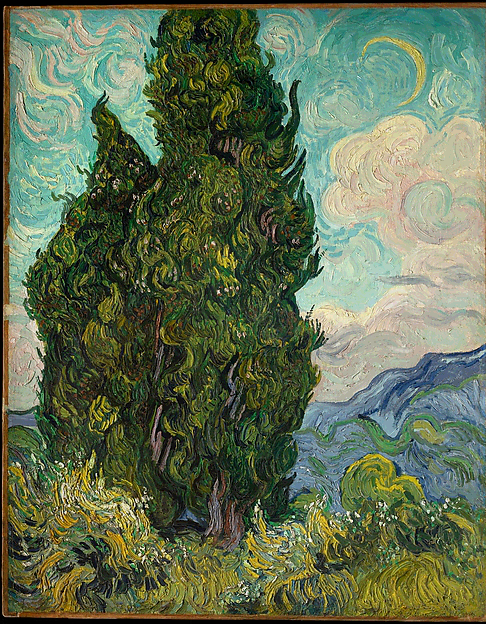
\includegraphics{image_femme_dans_cypres.png}
\caption{`image\_femme\_dans\_cypres.png'}
\end{figure}

\begin{itemize}
\tightlist
\item
  Image secret / cachée extraite après stéganographie :
\end{itemize}

\begin{figure}
\centering
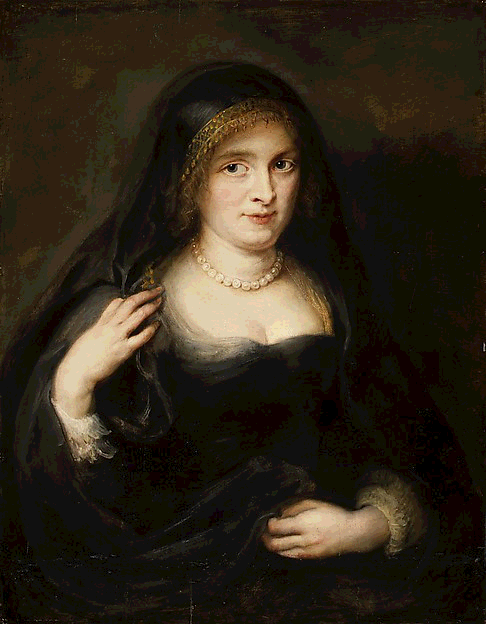
\includegraphics{image_cache_image_femme_dans_cypres.png}
\caption{`image\_cache\_image\_femme\_dans\_cypres.png'}
\end{figure}


    % Add a bibliography block to the postdoc
    
    
    
    \end{document}
